\documentclass[12pt,a4paper,twoside]{book}
\usepackage{graphicx}
\usepackage[utf8]{inputenc}
\usepackage[british]{babel}
\usepackage{hyperref}
\usepackage{indentfirst}
\usepackage{amssymb}
\usepackage{amsmath}
\usepackage{latexsym}
\usepackage{lipsum}
\usepackage{tikz}
\usepackage{amsthm}
\usepackage{algorithm}
\usepackage{algpseudocode}
\usepackage{stmaryrd}
\usepackage{listings}
\usepackage{xcolor, colortbl}
\usepackage{pgfgantt}
\usepackage{dirtree}
\usepackage{todonotes}
\usepackage{bussproofs}
\usepackage{mathtools}
\usepackage{msc}
\usepackage{subcaption}
\usepackage{macros}
\usepackage[a4paper,inner=3.5cm,outer=2.5cm]{geometry}
\usepackage[titletoc,title,toc,page]{appendix}
\usepackage{verbatim}
\usepackage{placeins}
\usepackage{parskip}
\usepackage{blindtext}
\usepackage{chngcntr}
\counterwithin{table}{chapter}
\usepackage{newlfont}
\usepackage{fancyhdr}
\usepackage{float}
\usepackage[capitalize,noabbrev]{cleveref}
\usepackage{soul}
\usepackage[font=footnotesize,labelfont=bf]{caption}
\usepackage{multirow}
\usepackage{pdfpages}
\usepackage{sansmath}
% \usepackage{hyphenat}
% \hyphenation{mate-mati-ca recu-perare}

\newcommand{\rom}[1]{\uppercase\expandafter{\romannumeral #1\relax}}

\newtheorem{theorem}{Theorem}
\newtheorem{lemma}{Lemma}
\newtheorem{corollary}{Corollary}
\theoremstyle{definition}
\newtheorem{example}{Example}

\usetikzlibrary{automata,arrows,positioning,shapes,snakes}
\usetikzlibrary{calc,matrix,decorations.pathmorphing}
\usetikzlibrary{shapes.geometric,arrows.meta}
\pgfmathtruncatemacro\distance{1}

\definecolor{green}{rgb}{0,0.5,0}
\definecolor{red}{rgb}{1,0,0}
\definecolor{yellow}{rgb}{0.5,0.5,0}
\definecolor{codeashgrey}{rgb}{0,0.6,0}
\definecolor{codegray}{rgb}{0.5,0.5,0.5}
\definecolor{codepurple}{rgb}{0.58,0,0.82}
\definecolor{backcolour}{rgb}{0.95,0.95,0.92}
\definecolor{ashgrey}{rgb}{0.7, 0.75, 0.71}

\lstdefinestyle{mystyle}{
    backgroundcolor=\color{backcolour},
    commentstyle=\color{codeashgrey},
    keywordstyle=\color{magenta},
    numberstyle=\tiny\color{codegray},
    stringstyle=\color{codepurple},
    basicstyle=\ttfamily\footnotesize,
    breakatwhitespace=false,
    breaklines=true,
    captionpos=b,
    keepspaces=true,
    numbers=left,
    numbersep=5pt,
    showspaces=false,
    showstringspaces=false,
    showtabs=false,
    tabsize=2
}

\lstset{style=mystyle}

\theoremstyle{definition}
\newtheorem{definition}{Definition}[section]

\theoremstyle{definition}
\newtheorem{exmp}{Example}[section]

\title{On the Implementability of Global Types}
\author{Student: Gabriele Genovese Supervisor: Cinzia Di Giusto}
\date{\today}

\begin{document}

\begin{titlepage}
\begin{center}
    \includegraphics[width=6.5cm,height=4.7cm]{img/unibo.png}
    
    \vspace{10mm}
   
    {\large{\bf{Dipartimento di Informatica - Scienza e Ingegneria}}} 
    
    \vspace{5mm}
    
    {\Large{\bf{Corso di Laurea Magistrale in Informatica}}}
    
    \vspace{15mm}
    
    {\Huge{\bf On the Implementability }}\\
    
    \vspace{3mm}
    
    {\Huge{\bf of Global Types}}\\
   
    \vspace{3mm}
\end{center}

\vspace{10mm}

\begin{minipage}[t]{0.45\textwidth}
    
    {\Large{\bf Relatore: \\ Prof. Ivan Lanese}}
    
    \vspace{3mm}
    
    {\Large{\bf Correlatori:\\Prof. Cinzia Di Giusto\\Prof. Étienne Lozes}}
\end{minipage}
\hfill
\begin{minipage}[t]{0.37\textwidth}\raggedleft
    {\Large{\bf Presentata da: \\ Gabriele Genovese}}\\
    {\Large{\bf Contro-relatore: \\ Luca Padovani}}
\end{minipage}

\vspace{25mm}
\rule[0.5cm]{15.8cm}{0.6mm}

\begin{center}
    {\large{\bf Sessione II Ottobre 2025 \\}}
    {\large{\bf Anno Accademico 2024/2025\\}}
\end{center}

\end{titlepage}

\pagenumbering{roman}

\thispagestyle{plain}
\restoregeometry
\topmargin=6.5cm
\begin{flushright}
\emph{
\LARGE{Qualcosa}%\\\vspace{2mm}
% \LARGE{Il diavolo sta nei dettagli}%\\\vspace{2mm}
% \LARGE{su più righe}
}
\end{flushright}

\newpage~\thispagestyle{plain}~\newpage

\phantomsection
\addcontentsline{toc}{chapter}{Abstract}
\chapter*{Abstract}
Behavioural types define how information is exchanged in distributed systems.
An example are Multiparty Session Types (MPST), which describe interactions between multiple participants
using global protocols and their local counterparts. Ensuring correct implementation,
including deadlock freedom and session conformance, is a central concern in MPST.
While most research targets peer-to-peer communication, real-world systems often
use different communication models such as mailbox-based or causally ordered messaging.
A key challenge is that protocols valid in one model may fail in another.
In this work, we develop a flexible MPST framework parameterized by different network
semantics, including asynchronous, peer-to-peer, causal ordering, and synchronous.
We study the implementability problem from a broad semantic perspective, aiming to
understand its fundamental limits. My contributions include a survey
of related work, a proof of undecidability for weak implementability under synchronous
semantics, and enhancements to the \textsc{ReSCu} tool for checking deadlock freedom in
synchronous systems. This approach embeds communication models as a parameter, and it
provides a basis for verifying distributed systems beyond classical settings.

\thispagestyle{plain}
\topmargin=-1cm
\cleardoublepage
\phantomsection
\addcontentsline{toc}{chapter}{Contents}
\tableofcontents
\thispagestyle{empty}
\cleardoublepage
\phantomsection
\addcontentsline{toc}{chapter}{List of Tables}
\listoftables
\thispagestyle{empty}
\cleardoublepage
\phantomsection
\addcontentsline{toc}{chapter}{List of Figures}
\listoffigures
\thispagestyle{empty}
\cleardoublepage
\phantomsection
\addcontentsline{toc}{chapter}{List of Listings}
\lstlistoflistings
\thispagestyle{empty}
\newpage~\newpage

\pagenumbering{arabic}
% \setcounter{chapter}{-1}
\raggedbottom

\chapter{Introduction} \label{chap:intro}
\pagestyle{plain}
\setcounter{page}{1}

Informally, a \textit{distributed system} is a collection of independent 
computing entities (interchangeably called processes, actors, 
nodes, or participants) that communicate and coordinate their 
actions through message passing over a medium of communication 
(typically an \textbf{asynchronous network}), with the goal of solving a 
common problem. For example, a client-server application can be seen 
as a form of distributed system, where the shared objective is to provide 
services to an end user.

Distributed systems address a wide range of challenges which are 
difficult to solve without such an architecture, for example reliability
under failures safety in critical systems, and consistency of data.
% Being able to \textbf{scale} to handle large volumes of incoming requests 
% would be nearly impossible without distributed systems. Likewise, achieving 
% \textbf{fault-tolerant} and high-performance applications would be 
% extremely difficult without them. 
% For these reasons,
Distributed systems are 
widely adopted in domains such as \textit{cloud computing}, critical 
infrastructures, and telecommunication-oriented applications (i.e.\ 
autonomous cars, aerospace systems, etc.). Given their ubiquity, it is 
crucial to study every aspect of their \textbf{design}, \textbf{execution}, 
and \textbf{verification}.

One recurring difficulty is writing \textbf{correct programs} in this 
context. Avoiding programming and logical errors is inherently hard, even 
for experienced developers. To mitigate this, many abstractions have been 
introduced, and computer scientists have focused their efforts on developing 
\textit{formal frameworks} that provide developers with guarantees about 
their programs. Formal methods for distributed systems offer 
mathematically rigorous techniques to specify, design, and 
verify such systems. They are valuable during development, helping 
detect errors early, and during analysis, enabling the study of critical 
properties such as \textbf{safety}, \textbf{liveness}, and 
\textbf{deadlock-freedom}. Two primary verification approaches are 
\textit{model checking} and \textit{by-construction} verification. Model 
checking systematically explores a system's state space to confirm 
properties, while by-construction verification guarantees correctness 
through the design process itself, preventing errors from being introduced. 

There exists several models to reason about distributed systems.
Different model are specialized in different aspects of a system, and we
are interested in the ones about the exchange of information, such as
Calculus of Communicating Systems (CCS), the $\pi$-calculus, and Petri nets.
In this work, however, we focus on 
\textit{Multiparty Session Types} (MPST)~\cite{honda2008multiparty} 
and \textit{choreographies}~\cite{montesi2014choreographic}, 
since these formalisms place particular emphasis on structured and 
verifiable communication protocols, making them especially well suited 
for protocol design.
In MPST, communication is specified by a \emph{global type}, which 
describes the entire interaction among participants. 
This global type is then \emph{projected} into 
\emph{local types}, one for each participant. 
Local types serve as contracts that guarantee each component is compliant to 
the described protocol, therefore ensuring certain properties, 
such as deadlock-freedom, at compile time. 
The implementability problem in MPST is comparable to verifying 
whether a given global type can be correctly projected into local 
types, preserving the intended behavior.

\section{Goal}
The goal of this work is to study the \textbf{implementability
problem}, which concerns whether a global specification can be
faithfully realized by a set of \textit{local processes} in a
distributed system.
In essence, it asks: does an implementation really \textbf{respect}
the behavior described by a given specification model?

To illustrate the relevance of this problem, consider the following
example.
\begin{example}
Given four processes $A, B, C, D$ distributed over
a network, and four messages $x, y, z, w$ to be exchanged according to
the description in Listing~\ref{lst:not-impl-exm}, is it possible to
implement it in a real world system?

\begin{lstlisting}[caption={Example specification of message exchanges},
                   label={lst:not-impl-exm},
                   keywordstyle=\color{blue}\bfseries,morekeywords={sends,If,then}]
A sends B either message x or y.

If A sends B message x,
    then C sends D message z.

If A sends B message y,
then C sends D message w.
\end{lstlisting}
While the specification can be expressed using several of the
formalisms mentioned earlier, only some are capable of revealing that
it is, in fact, impossible to implement in a real distributed system.
The reason is that process $C$ cannot determine which message to send
to $D$ without knowing which message $A$ sent to $B$, because this 
information is not locally available to $C$.
\end{example}

This problem is examined from a theoretical
perspective to provide a more formal and precise understanding of
the fundamental limits that exist and why syntactical constrains
of certain models works.
In this work, we use an \textit{automata-based} approach to Global Types. 
This formalism is designed to be highly modular, 
incorporating various \textit{network semantics} (such as asynchronous, 
peer-to-peer, causal ordering, and synchronous semantics) as explicit 
parameters of the framework. This parameterization allows flexible 
analysis of different communication models within a unified setting.

The main contributions of this work are: 
\begin{itemize}
    \item a \textbf{state-of-the-art} review, highlighting
    existing research and results in this particular domain and giving
    perspective to our work;
    \item we prove \textbf{undecidability} of the \textit{weak implementability} 
    problem under the synchronous semantics of our framework;
    \item we extend and improve the model-checking tool \textsc{ReSCu}~\cite{rescurepo},  
    enabling verification of \textit{deadlock-freedom} and \textit{progress} 
    for synchronous systems.
\end{itemize}
The thesis begins with a brief overview of the main objects and problem
in Section~\ref{sec:sota} with a state-of-the-art
overview, presented in a general and accessible manner, avoiding
formal definitions and proofs. Chapters~\ref{sec:pre} and
\ref{sec:proof} then introduce the necessary formal definitions,
followed by the main theoretical contribution and in 
Chapter~\ref{sec:rescu} the practical contributions of
this work. Finally, Chapter~\ref{sec:end} presents concluding
remarks and outlines possible directions for future research and
development.

\section{Brief overview}\label{sec:sota}
In this overview, we give a brief understanding of the
state of the art regarding MSCs and the implementability 
(or realizability) problem.

\subsection{Message Sequence Charts}
Message Sequence Charts (MSCs) are a standardized graphical formalism,
introduced in 1992 \cite{MSCStandard}, used to describe trace languages for specifying
communication behavior. Thanks to their simplicity and intuitive
semantics, MSCs have been widely adopted in industry.
Figure~\ref{fig:msc-cli-ser} illustrates a simple example based on a
minimal client–server architecture. An extension of this formalism,
known as High-Level Message Sequence Charts (HMSCs), was later
introduced \cite{HMSCStandard}. HMSCs enable the definition of
MSCs as nodes connected by transitions and are used to model more
complex patterns of message flows by capturing sequences, alternatives,
or iterations of atomic MSC scenarios.

\begin{figure}[!ht]
\centering
\begin{msc}[draw frame=none, draw head=none, msc keyword=, head height=0px, label distance=0.5ex, foot height=0px, foot distance=0px]{}
	\declinst{P1}{Client}{}
	\declinst{P2}{Server}{}

	\mess{request}{P1}{P2}
	\nextlevel
	\mess{answer}{P2}{P1}
\end{msc}
\caption{Simple example of a client-server architecture.}
\label{fig:msc-cli-ser}
\end{figure}

% TODO: rimanere ad alto livello
% ma aggiungere reference alle definizioni formali 
% nella parte di definizioni formali fare un confronto.
% citare il confronto qua e rimandare dopo

\subsubsection{The realizability problem for MSCs}

The \emph{realizability problem} was first introduced for MSC languages 
in~\cite{alur2000inference,alur2003inference}. It asks whether there exists a distributed 
implementation that can realize all behaviors of a finite set of MSCs 
without introducing additional ones. A stronger variant, called 
\emph{safe realizability}, requires the implementation to also be \textbf{deadlock-free}. 
% In this setting, distributed implementations are defined using communicating 
% automata with explicit accepting states, and deadlock-freedom corresponds 
% to the ability to reach an accepting state from any reachable configuration. 

\subsubsection{Hierarchy of communication model's semantics}
With MSCs, \cite{di2023partial} presents some interesting communication
semantics. I will describe a few of them informally, using examples to
highlight the differences from the main semantics considered in this work,
which is \verb|synch|, that is also the only one formally defined in 
Definition~\ref{def:synch}. Some examples are
shown in Figure~\ref{fig:msc_examples}. These examples can be verified that 
are really part of the corresponding communication semantics with an online
tool for MSC~\cite{MSCTool}. Figure~\ref{fig:coms} shows the hierarchy
of the communication semantics defined. % TODO: dare più contesto alla figura

% TODO: rsc =/= sync (messaggi orfani)


\begin{figure}[!ht]
\centering
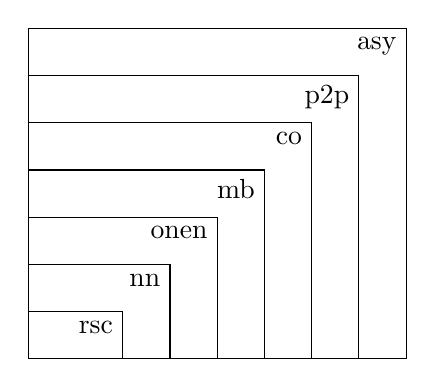
\begin{tikzpicture}[scale=0.6]
  % list of labels in order (from smallest to largest)
%   \def\labels{{rsc,nn,onen,mb,co,p2p,asy}}
  % loop to draw nested squares
  \foreach [count=\i] \lab in {rsc,nn,onen,mb,co,p2p,asy} {
    \draw (0,0) rectangle (\i+1,\i);
    \node[anchor=north east] at (\i+1,\i) {\lab};
  }
\end{tikzpicture}
\caption{Hierarchy of communication model semantics.}
\label{fig:coms}
\end{figure}

% TODO: dire che la proiezione non è monotona e che quindi non può essere
% passata ad altre semantica (ma altre sì tipo weak-k-synchronizability)

\begin{figure}[!ht]
    \centering
    \begin{tabular}{cc}
        \scalebox{0.6}{%
        \begin{msc}[draw frame=none, draw head=none, msc keyword=, 
                    head height=0px, label distance=0.5ex, 
                    foot height=0px, foot distance=0px]{}
            \declinst{p}{p}{}
            \declinst{q}{q}{}

            \mess[pos=0.2]{$m_1$}{p}{q}[2]
            \nextlevel
            \mess[pos=0.8]{$m_2$}{p}{q}
        \end{msc}%
        } &
        \scalebox{0.5}{%
        \begin{msc}[draw frame=none, draw head=none, msc keyword=, 
                    head height=0px, label distance=0.5ex, 
                    foot height=0px, foot distance=0px]{}
            \declinst{p}{p}{}
            \declinst{q}{q}{}
            \declinst{r}{r}{}

            \mess[pos=0.15]{$m_1$}{p}{r}[3]
            \nextlevel
            \mess[pos=0.8]{$m_2$}{p}{q}
            \nextlevel
            \mess[pos=0.8]{$m_3$}{q}{r}
        \end{msc}%
        } \\
        (a) asynchronous (\verb|asy|) & (b) peer-to-peer (\verb|p2p|) \\
        \scalebox{0.5}{%
        \begin{msc}[draw frame=none, draw head=none, msc keyword=, 
                    head height=0px, label distance=0.5ex, 
                    foot height=0px, foot distance=0px]{}
            \declinst{p}{p}{}
            \declinst{q}{q}{}
            \declinst{r}{r}{}
            \declinst{s}{s}{}

            \mess[pos=0.1]{$m_4$}{p}{s}[4]
            \nextlevel
            \mess[pos=0.8]{$m_1$}{p}{q}
            \nextlevel
            \mess[pos=0.2]{$m_2$}{r}{q}
            \nextlevel
            \mess[pos=0.8]{$m_3$}{r}{s}
        \end{msc}%
        } &
        \scalebox{0.6}{%
        \begin{msc}[draw frame=none, draw head=none, msc keyword=, 
                    head height=0px, label distance=0.5ex, 
                    foot height=0px, foot distance=0px]{}
            \declinst{p}{p}{}
            \declinst{q}{q}{}
            \declinst{r}{r}{}

            \mess{$m_1$}{p}{q}
            \nextlevel
            \mess{$m_2$}{q}{r}
        \end{msc}%
        } \\
        (c) mailbox (\verb|mb|) & (d) synchronous (\verb|synch|)
    \end{tabular}
    \caption{MSCs' Examples for various communication models.}
    \label{fig:msc_examples}
\end{figure}

\paragraph{Fully asynchronous}

In the fully asynchronous communication model (\verb|asy|), messages can be 
received at any time after they have been sent, and send events are 
non-blocking. This model can be viewed as an unordered ``bag'' in which 
all messages are stored and retrieved by processes when needed. It is also 
referred to as \emph{non-FIFO}. The formal definition coincides with that of 
an MSC. Figure~\ref{fig:msc_examples}.a illustrates an example of asynchronous 
communication.

\paragraph{Peer-to-peer} 
In the peer-to-peer (\verb|p2p|) communication model, any two messages sent from one 
process to another are always received in the same order as they are sent.
Alternative names are FIFO. An example is shown in Figure~\ref{fig:msc_examples}.b.

% A p2p-MSC is an MSC $M = (E,\to, \lhd, \lambda)$ where, for any two send events $s$ 
% and $s'$ such that $\lambda(s) \in \text{send}(p, q, \_), \lambda(s') in \text{send}(p, q, \_)$, 
% and $s \to^+ s'$, one of the following holds:
% - either $s, s' \in \text{matched}(M)$ with $s \lhd r$ and $s' \lhd r'$ and 
% $r \to^+ r'$,
% - or $s' \in \text{unmatched}(M)$.
% Note that we cannot have two messages $m 1$ and $m 2$, both sent by $p$ to $q$, 
% in that order, such that $m 1$ is unmatched and $m 2$ is matched; unmatched 
% message $m 1$ excludes the reception of any later message.

\paragraph{Causally ordered}
In the causally ordered (\verb|co|) communication model, messages are delivered 
to a process in accordance with the causal dependencies of their emissions. 
In other words, if there are two messages $m_1$ and $m_2$ with the same recipient, 
such that there exists a causal path from $m_1$ to $m_2$, then $m_1$ must be received 
before $m_2$. This notion of causal ordering was first introduced by Lamport under the 
name ``happened-before'' relation. In Figure~\ref{fig:msc_examples}.b, this 
causality is violated: $m_1$ should be received before $m_3$. Causal delivery 
is commonly implemented using Lamport's logical clock algorithm \cite{lamport2019time}.

% An MSC $M = (E, \to, \lhd, \lambda)$ is causally ordered if, for any two send $s$ and 
% $s'$, such that $\lambda(s) \in \text{send}(\_, q, \_), \lambda(s') \in \text{send}(\_, q, \_)$, and 
% $s \leq_{\text{hb}} s'$:
% - either $s, s' \in \text{matched}(M)$ and $r \to^* r'$, with $r$ and $r'$ receive 
% events such that $s \lhd r$ and $s' \lhd r'$.
% - or $s' \in \text{unmatched}(M)$.

% Note that in a \verb|co|-MSC we cannot have two send events $s$ and $s'$ addressed 
% to the same process, such that $s$ is unmatched, $s'$ is matched, and 
% $s \leq_{\text{hb}} s'$.

\paragraph{Mailbox}
In this model, any two messages sent to the same process, regardless of the sender, 
must be received in the same order as they are sent. If a process receives $m_1$ 
before $m_2$, then $m_1$ must have been sent before $m_2$. \verb|mb| coordinates all 
the senders of a single receiver. This model is also called FIFO $n-1$.
In Figure~\ref{fig:msc_examples}.c, an example for this communication model is shown.

% An MSC $M = (E, \to, \lhd, \lambda)$ is a \verb|mb|-MSC if it has a linearization 
% $\rightsquigarrow$ where, for any two send events $s$ and $s'$, such 
% that $\lambda (s) \in \text{send}(\_,q,\_), \lambda (s') \in \text{send}(\_,q,\_)$, and 
% $s \rightsquigarrow s'$
% - either $s,s' \in \text{matched}(M)$ and $r \rightsquigarrow r'$, where 
% $s \lhd r$ and $s' \lhd r'$,
% - or $s' \in \text{unmatched}(M)$.

\paragraph{FIFO 1-n}
This model (\verb|onen|) is the dual of \verb|mb|, it coordinates a sender with all the 
receivers. Any two messages sent by a process must be received in the same 
order as they are sent. These two messages might be received by different 
processes and the two receive events might be concurrent.

% An MSC $M = (E, \to, \lhd, \lambda)$ is a \verb|onen|-MSC if it has a linearization 
% $\rightsquigarrow$ where, for any two send events $s$ and $s'$, such 
% that $\lambda (s) \in \text{send}(p,\_,\_), \lambda (s') \in \text{send}(p,\_,\_)$ and 
% $s \to^+ s'$ (which implies $s \rightsquigarrow s'$)
% - either $s,s' \in \text{matched}(M)$ and $r \rightsquigarrow r'$, with 
% $r$ and $r'$ receive events such that $s \lhd r$ and $s' \lhd r'$,
% - or $s' \in \text{unmatched}(M)$.

\paragraph{FIFO n-n}
In this model (\verb|nn|), messages are globally ordered and delivered according to 
their emission order. Any two messages must be received in the same order 
as they are sent. These two messages might be sent or receives by any process 
and the two send or receive events might be concurrent. The FIFO \verb|n-n| 
coordinates all the senders with all the receivers.

% An MSC $M = (E, \to, \lhd, \lambda)$ is a \verb|nn|-MSC if it has a linearization 
% $\rightsquigarrow$ where, for any two send events $s$ and $s'$, such 
% that $s \rightsquigarrow s'$
% - either $s, s' \in \text{matched}(M)$ and $r \rightsquigarrow r'$, with $r$ 
% and $r'$ receive events such that $s \lhd r$ and $s' \lhd r'$,
% - or $s' \in \text{unmatched}(M)$.

\paragraph{Synchronous}
The synchronous (\verb|synch|) communication model imposes 
the existence of a scheduling such that any send event is 
immediately followed by its corresponding receive event. 
An example for this communication model is shown in Figure~\ref{fig:msc_examples}.d.
A formal definition is given later for this semantic (Definition~\ref{def:synch}).

\subsection{Multiparty Session Types}
Multiparty Session Types (MPST)~\cite{honda2008multiparty} 
provide a type-theoretic framework to specify and verify communication 
protocols among multiple participants. They ensure that communication 
follows a predefined structure, preventing errors such as deadlocks, 
orphan messages, and unspecified receptions. The 
\textbf{global specification} describes the overall communication 
protocol. From this, one derives the \textbf{local behaviors} of each 
participant via a \emph{projection} operation. The system's 
\textbf{processes} form the \emph{implementation}, defining how 
participants interact. With the definition of a \emph{typing system} 
and suitable \emph{type-checking rules}, one ensures that the 
implementation conforms to the local specification, thereby 
guaranteeing properties such as \emph{well-formedness}.  

% In this setting, the analogue of realizability is often called 
% \emph{session fidelity}: a property ensuring that the combined local 
% types behave exactly according to the global type. When the global 
% type satisfies syntactic restrictions, its projection is guaranteed 
% to be both realizable and deadlock-free, which corresponds to safe 
% realizability in the MSC setting.  

\subsubsection{Projectability}
A central notion in MPST is \emph{projectability}, which asks whether 
a global type can be faithfully projected into local specifications for 
each participant. If projection succeeds, the resulting local types 
interact without mismatches or unintended behaviors, effectively 
bridging global specifications and distributed implementations~\cite{honda2008multiparty}.  
Projectability is, therefore, comparable to the implementability
problem as have the same aim.
Projection algorithms, however, often reject natural protocols that 
fail to meet restrictive syntactic conditions. This difference between 
expressivity and safety has motivated extensions of the theory, with 
\cite{castagna2012global} being the only algorithm aiming for full 
completeness.

\subsubsection{Mixed and Sender driven choice}
A key restriction appears in branching. In the original framework \cite{honda2008multiparty,carbone2012structured}, 
choice is \textbf{sender-driven}: the first sender dictates the branch, 
ensuring safety but excluding many common patterns where multiple 
participants influence the decision~\cite{carbone2012structured}.  
Allowing \textbf{mixed choice} increases expressivity by permitting 
several initiators, but it also makes the implementability problem 
undecidable in general~\cite{barbanera2020choreography}.  

\subsection{Choreographies}
%todo


\subsection{Reduction to synchronous semantic}
The main idea of this work is that reasoning about implementability 
becomes more tractable under \emph{synchronous} 
semantics for automata-based solutions to the implementability problem. 
In synchronous communication, send and receive actions 
are tightly coupled, effectively removing nondeterminism 
caused by asynchronous message buffering. Several results exploit this 
observation by reducing the implementability problem under richer 
communication models (e.g.\ asynchronous or peer-to-peer FIFO) to the 
simpler synchronous case~\cite{alur2005realizability,di2023partial}.

Formally, one can show that if a global type is implementable in 
synchronous semantics, then under certain conditions it is also 
implementable in more general models such as peer-to-peer or mailbox 
semantics. This reduction requires constraints such as 
\emph{orphan-freedom} (no message is left unmatched) and
\emph{deadlock-freedom}.
The following theorem, currently a work in progress by my supervisors \cite{di2025realisability}, 
provides a characterization of a connection between 
peer-to-peer semantics and synchronous semantics:

\begin{theorem}
	A global type $G$ is implementable in \verb|p2p| iff:
	\begin{enumerate}
		\item $L_{\text{p2p}}(proj(G))$ is a set of sync MSCs;
		\item $proj(G)$ is orphan-free in p2p;
		\item $L_{\text{p2p}}(proj(G))$ is deadlock-free;
		\item $G$ is implementable in sync.
	\end{enumerate}
\end{theorem}

This result highlights the central role of synchronous semantics as a 
\emph{core model}: implementability in peer-to-peer systems 
can be reduced to the synchronous case provided the additional safety 
conditions are met. My own contribution focuses on the last item of the 
theorem, namely the problem of checking whether a given global type is 
implementable in synchronous semantics. This question is at the heart 
of the undecidability results presented in Section~\ref{sec:proof}, 
and motivates the need for the identification of new subclasses that 
enable new verification techniques along with tool support.

% \input{content/sota}

\chapter{Preliminaries}\label{sec:pre}
In this section, the fundamental concepts and definitions necessary 
to contextualize the main contributions of this work are presented. 
We, first, introduce automaton, executions, and
Message Sequence Charts (MSC), followed by 
an examination of communication model's semantics that are particularly 
interesting. 
Then, the notions of Global Type and Realisability are 
defined within the scope of this work, along with the foundational 
elements required to understand the theoretical contributions.

\section{Standard notions on automata}
For a string $s$, let $s^l$ denote the $l$-th character of the string.

\bigskip

\begin{definition}[NFA]\label{def:nfa}
A non-deterministic finite automaton (NFA) is a tuple  
$\mathcal{A} = (Q, \Sigma, \delta, q_0, F)$, where $Q$ is a finite set of  
states, $\Sigma$ is a finite alphabet,  
$\delta : Q \times (\Sigma \cup \{\varepsilon\}) \to Q$ is the transition  
relation, $q_0 \in Q$ is the initial state, and $F \subseteq Q$ is the set  
of accepting states.  

We write $\delta^*(s,w)$ to denote the set of states $s'$ reachable from  
$s$ along a path labelled with $w$. The language accepted by $\mathcal{A}$,  
denoted $\mathcal{L}_{\text{words}}(\mathcal{A})$, is the set of words  
$w \in \Sigma^*$ such that $\delta^*(q_0,w) \cap F \neq \emptyset$.  
\end{definition}

\bigskip

\begin{definition}[DFA]\label{def:dfa}
A deterministic finite automaton (DFA) is an NFA where the transition  
relation $\delta$ is a partial function  
$\delta : Q \times \Sigma \to Q$. The DFA is complete if $\delta$ is  
total.  

% Every DFA $\mathcal{A} = (Q, \Sigma, \delta, q_0, F)$ accepts the same  
% language as the complete DFA $\mathcal{A}' = (Q \cup \{\perp\}, \Sigma,  
% \delta', q_0, F)$, where $\delta'(q,a) = \perp$ if $\delta(q,a)$ is  
% undefined, and $\delta'(\perp,a) = \perp$.  
\end{definition}

\bigskip

\begin{definition}[Determinization]\label{def:det}
To every NFA $\mathcal{A} = (Q, \Sigma, \delta, q_0, F)$, we associate  
the DFA $\text{det}(\mathcal{A}) = (Q', \Sigma, \delta', q'_0, F')$,  
where $Q' = 2^Q$, $q'_0 = \{q_0\}$, $F'$ is the set of subsets of $Q$  
that contain at least one accepting state, and $\delta'$ is defined by  
$\delta'(S,a) = \bigcup\{\delta^*(s,a) \mid s \in S\}$ for all  
$S \in Q'$, $a \in \Sigma$.  
\end{definition}

We write $\acceptcompletion{\mathcal A}{}$ for the automaton obtained
from $\mathcal A$ by setting $F=Q$.

% \begin{definition}[Product NFA]\label{def:product-nfa}
% Given two NFAs $\mathcal{A}_1 = (Q_1, \Sigma, \delta_1, q_{0,1}, F_1)$ and  
% $\mathcal{A}_2 = (Q_2, \Sigma, \delta_2, q_{0,2}, F_2)$, the product NFA is  
% defined as  
% \[
% \mathcal{A}_1 \otimes \mathcal{A}_2 \stackrel{\text{def}}{=}  
% (Q_1 \times Q_2, \Sigma, \delta, (q_{0,1}, q_{0,2}), F_1 \times F_2),
% \]  
% where the transition relation $\delta$ is defined as follows:  

% \begin{itemize}  
%   \item for all $(s_1,s_2) \in Q_1 \times Q_2$, $a \in \Sigma$,  
%   $(s'_1,s'_2) \in Q_1 \times Q_2$:  
%   $((s_1,s_2),a,(s'_1,s'_2)) \in \delta$  
%   iff $(s_1,a,s'_1) \in \delta_1$ and $(s_2,a,s'_2) \in \delta_2$.  

%   \item for all $(s_1,s_2) \in Q_1 \times Q_2$, $(s'_1,s'_2) \in Q_1 \times Q_2$:  
%   $((s_1,s_2),\varepsilon,(s'_1,s'_2)) \in \delta$  
%   iff $(s_1,\varepsilon,s'_1) \in \delta_1$ or $(s_2,\varepsilon,s'_2) \in \delta_2$.  
% \end{itemize}  

% It holds that  
% $\mathcal{L}_{\text{words}}(\mathcal{A}_1 \otimes \mathcal{A}_2) =  
% \mathcal{L}_{\text{words}}(\mathcal{A}_1) \cap  
% \mathcal{L}_{\text{words}}(\mathcal{A}_2)$.  
% \end{definition}

% \begin{definition}[Dual DFA]\label{def:dual-dfa}
% If $\mathcal{A} = (Q, \Sigma, \delta, q_0, F)$ is a DFA, its dual is  
% defined as  
% \[
% \mathcal{A}^{\text{dual}} = (Q, \Sigma, \delta, q_0, Q \setminus F).
% \]  
% If $\mathcal{A}$ is complete, then  
% $\mathcal{L}_{\text{words}}(\mathcal{A}^{\text{dual}}) =  
% \Sigma^* \setminus \mathcal{L}_{\text{words}}(\mathcal{A})$.  
% \end{definition}

\section{Execution, Communication Models and MSC}
We assume a finite set of \emph{processes} 
$\Procs=\{p,q,\ldots,P1,P2,\ldots\}$ and a finite set of 
messages (labels) $\Msg=\{\msg_1,\msg_2,\ldots\}$.  
We consider two kinds of actions:  
\begin{itemize}
	\item \emph{send actions}, of the form $\send{p}{q}{\msg}$, 
	executed by process $p$ when sending message $\msg$ to $q$;  
	\item \emph{receive actions}, of the form $\recv{p}{q}{\msg}$, 
	executed by process $q$ when receiving $\msg$ from $p$.  
\end{itemize}

Furthermore, we write $\Act$ for the set $\Procs \times \Procs \times \{!,?\} \times \Msg$  
of all actions, and $\Actp$ for the subset of actions executable by $p$ 
(i.e., $\send{p}{q}{\msg}$ or $\recv{q}{p}{\msg}$).  
When processes are clear from the context, we abbreviate 
send and receive actions as $!\msg$ and $?\msg$, respectively.  

An \emph{event} $\event$ of a sequence of actions $w \in \Act^*$  
is an index $i \in \{1,\ldots,\length{w}\}$.  
It is a \emph{send event} (resp. \emph{receive event}) if $w[i]$  
is a send (resp. receive) action.  
We denote by $\sendeventsof{w}$ (resp. $\receiveeventsof{w}$)  
the set of send (resp. receive) events of $w$, and  
$\eventsof{w} = \sendeventsof{w} \cup \receiveeventsof{w}$.  
When all events are labelled with distinct actions, 
we identify an event with its action.  

\paragraph{Executions.}
An execution is a well-defined sequence of actions $e\in\Act^*$, where a
receive action is always preceded by a unique corresponding send action. % TODO : in che senso?

\bigskip

\begin{definition}[Execution]\label{def:execution}
An \emph{execution} over $\Procs$ and $\Msg$ is a sequence 
of actions $e \in \Act^*$ together with an injective mapping 
$\source_{e} : \receiveeventsof{e} \to \sendeventsof{e}$  
such that for each receive event $i$ labelled $\recv{p}{q}{\msg}$,  
its source $\source_{e}(i)$ is labelled $\send{p}{q}{\msg}$ and  
$\source_{e}(i) < i$.  
\end{definition}

For a set of executions $\mathcal{E}$, let 
$\prefixclosureof{\mathcal{E}}$ be the set of all prefixes 
of executions in $\mathcal{E}$.  
The \emph{projection} $\projofon{e}{p}$ of $e$ on process $p$  
is the subsequence of actions in $\Actp$.  
A send event $s$ is \emph{matched} if there exists a receive event $r$  
such that $\source(r) = s$.  
An execution is \emph{orphan-free} if all send events are matched,  
i.e., if $\source$ is surjective onto $\sendeventsof{e}$.  

\subsubsection*{Communication Models.}
In this thesis, we focus on a communication model: 
the synchronous model ($\synchmodel$).  
Nonetheless, this work forms part of a 
broader and more general project. Some results presented here 
naturally extend to a wide range of communication models, often requiring 
only mild additional assumptions. Please, refer to the related work chapter
(Chapter~\ref{sec:rel}, Section~\ref{sec:hier}).
From this perspective, we introduce a general definition of a communication 
model. 

\bigskip

\begin{definition}[Communication model]\label{def:communication-model}
A \emph{communication model} $\acommunicationmodel$  
is a set $\executionsofmodel{\acommunicationmodel}$ of executions.  
\end{definition}

In the \emph{synchronous model} $\synchmodel$,  
every send is immediately followed by its matching receive:  

\bigskip

\begin{definition}[$\synchmodel$]\label{def:synchronous}
An execution $e = (w,\source)$ belongs to 
$\executionsofmodel{\synchmodel}$ if for every send event 
$s \in \sendeventsof{e}$, the event $s+1$ is a receive event 
with $\source(s+1) = s$.  
\end{definition}
 
Furthermore, the \emph{source function} $\source_e$ is defined as follows.  

\bigskip

\begin{definition}[$\source$ function for $\synchmodel$]\label{def:src}
If $e$ is an execution in $\synchmodel$, then for every receive event $i$ 
we define $\source_e(i) = i-1$.
\end{definition}


\subsubsection*{Message Sequence Charts.}
While executions correspond to a total order of events in a system,  
message sequence charts (MSCs) provide a distributed view, using  
a partial order on events.  
For a tuple $\mmsc=(w_p)_{p\in\Procs}$, each $w_p \in \Actsp$ is a  
sequence of actions executed by process $p$, according to some  
total, locally observable order.  
We write $\eventsof{\mmsc}$ for the set  
$\{(p,i) \mid p \in \Procs \text{ and } 0 \leq i < \length{w_p}\}$.  
The label $\actionof{\event}$ of an event $\event=(p,i)$ is the action  
$w_p[i]$. The event $\event$ is a send (resp. receive) event if it is  
labelled with a send (resp. receive) action.  
We write $\sendeventsof{\mmsc}$ (resp. $\receiveeventsof{\mmsc}$)  
for the set of send (resp. receive) events of $\mmsc$. We also write  
$\messageof{\event}$ for the message sent or received at $\event$, and  
$\processof{\event}$ for the process executing $\event$.  
Finally, we write $\verticalorderstrict{\event_1}{\event_2}$ if there  
exists a process $p$ and indices $i<j$ such that  
$\event_1=(p,i)$ and $\event_2=(p,j)$.  

\bigskip

\begin{definition}[Message Sequence Chart]\label{def:msc}
	An \emph{MSC} over $\Procs$ and $\Msg$ is a tuple 
	$\mmsc = \big((w_p)_{p\in\Procs},\source\big)$ where
    \begin{enumerate}
        \item for each process $p$, $w_p\in\Actsp$ is a finite sequence 
			of actions;
		\item $\source : \receiveeventsof{\mmsc} \to \sendeventsof{\mmsc}$ is 
			an injective function from receive events to send events such that
			for all receive event $\event$ labelled with $\recv{p}{q}{\msg}$,
			$\source(\event)$ is labelled with $\send{p}{q}{\msg}$.
    \end{enumerate}
\end{definition}

For an execution $\execution$,  $\mscof{\execution}$ is the MSC 
$\big((w_p)_{p\in\Procs},\source\big)$ where $w_p$ is the 
subsequence of $\execution$ restricted to the actions of $p$,
and $\source$ is the lifting of $\source_{\execution}$ to the
events of $(w_p)_{p\in\Procs}$.

\bigskip

\begin{example}\label{exmp:msc}
Consider the MSC depicted in Figure~\ref{fig:msc-exmp}.  
It consists of $\Procs=\{p,q,r\}$ and $\Msg=\{\msg_1,\msg_2,\msg_3\}$
with $\mmsc=((w_p,w_q,w_r),\source)$, where
$w_p = {}!\msg_1{}?\msg_2$, 
$w_q = {}?\msg_1{}!\msg_2{}!\msg_3$, 
$w_r = {}?\msg_3$,
$\source((p,2)) = (q,2)$,
$\source((q,1)) = (p,1)$, and
$\source((r,1)) = (q,3)$.

\begin{figure}[!ht]
\centering
\begin{msc}[draw frame=none, draw head=none, msc keyword=, head height=0px, label distance=0.5ex, foot height=0px, foot distance=0px]{}
	\declinst{p}{p}{}
	\declinst{q}{q}{}
	\declinst{r}{r}{}

	\mess{$m_1$}{p}{q}
	\nextlevel
	\mess{$m_2$}{q}{p}
	\nextlevel
	\mess{$m_3$}{q}{r}
\end{msc}
\caption{Simple example with an exchange of three messages.}
\label{fig:msc-exmp}
\end{figure}
\end{example}

Given a set of processes $\Procs$, an MSC 
$M=\big((w_p)_{p\in\Procs},\source\big)$ is said to be a 
\emph{prefix} of another MSC 
$M'=\big((w'_p)_{p\in\Procs},\source'\big)$, denoted by 
$M \prefixorder M'$, if the following conditions hold:  
\begin{itemize}
    \item for every $p \in \Procs$, the sequence $w_p$ is a prefix 
    of $w'_p$;  
    \item for every receive event $e$ of $M$, it holds that 
    $\source'(e)=\source(e)$.  
\end{itemize}

The \emph{concatenation} of two MSCs $M_1$ and $M_2$ is the MSC 
$M_1 \cdot M_2$ obtained by stacking $M_1$ vertically above $M_2$. 
Formally, let 
$M_1=((w_p^1)_{p\in\Procs},\source_1)$ and 
$M_2=((w_p^2)_{p\in\Procs},\source_2)$. Then:  
\begin{inparaenum}[(i)]
   \item for each process $p$, the sequence is 
   $w_p = w_p^1 \cdot w_p^2$;  
   \item the source function $\source$ is defined so that 
   $\source(e)=\source_i(e)$ for all receive events $e$ belonging 
   to $M_i$, with $i\in\{1,2\}$.  
\end{inparaenum}


\subsubsection*{Happens-before relation and linearisations}
In a given MSC $M$, an event $\event$ happens before $\event'$, if 
$\event$ and $\event'$ are events
of a same process $p$ and happen in that order on 
the timeline of $p$; $\event$ is send event matched by $\event'$; and
a sequence of such situations defines a path from $\event$ to $\event'$.

\bigskip

\begin{definition}[Happens-before relation]
Let $\mmsc$ be an MSC. The happens-before relation over $M$
is the binary relation $\happensbeforestrict$ defined as 
the least transitive relation over $\eventsof{\mmsc}$ such that:
\begin{itemize}
   \item for all 
   $p,i,j$, if $i<j$, then $(p,i)\happensbeforestrict (p,j)$, and
   \item for all receive events 
   $\event$, $\source(\event) \happensbeforestrict \event$.
\end{itemize}
\end{definition}

\bigskip

\begin{example}
Consider the Example~\ref{exmp:msc}. 
The following happens-before relations are valid:
$${}!\msg_1{}\happensbeforestrict {}?\msg_1 \happensbeforestrict {}!\msg_2
\happensbeforestrict {}!\msg_3 \happensbeforestrict {}?\msg_3$$
and
$${}!\msg_1{}\happensbeforestrict {}?\msg_1 \happensbeforestrict {}!\msg_2
\happensbeforestrict {}?\msg_2.$$
\end{example}

\bigskip

\begin{definition}[Linearisation]\label{def:linearisation}
	A \emph{linearisation} of an MSC $\mmsc$ is a
	total order $\alinearisation$ on $\eventsof{\mmsc}$
	that refines $\happensbeforestrict$:  for all events $\event,\event'$, 
	if $\event\happensbeforestrict \event'$, then $\event\alinearisation \event'$. 
\end{definition}
We write $\linearisationsof{\mmsc}{}$ for the set of all linearisations
of $\mmsc$. 
We often identify a linearisation with the execution it induces.

\bigskip

\begin{example}\label{exmp:lin}
Considering the Example~\ref{exmp:msc},	
let $\mmsc$ be the MSC in Figure~\ref{fig:msc-exmp}. 
The elements of the set $\linearisationsof{\mmsc}{}$ are
$$!m_1?m_1!m_2?m_2!m_3?m_3,$$
$$!m_1?m_1!m_2!m_3?m_2?m_3,$$
$$!m_1?m_1!m_2!m_3?m_3?m_2.$$
\end{example}

Given an MSC $\mmsc$, we write 
$\linearisationsof{\mmsc}{\acommunicationmodel}$ to denote
$\linearisationsof{\mmsc}{}\cap\executionsofmodel{\acommunicationmodel}$;
the executions of $\linearisationsof{\mmsc}{\acommunicationmodel}$ 
are called the linearisations of $\mmsc$ in the communication 
model \verb|com|.

\bigskip

\begin{definition}[$\acommunicationmodel$-linearisable MSC]
	\label{def:linearisable-msc}
	An MSC $\mmsc$ is \textit{linearisable} in a communication 
	model $\acommunicationmodel$
	if $\linearisationsof{\mmsc}{\acommunicationmodel}\neq\emptyset$.
	We write $\mscsetofmodel{\acommunicationmodel}$ for the set of all MSCs 
	linearisable in $\acommunicationmodel$.
\end{definition}

\bigskip

\begin{example}
Consider the Example~\ref{exmp:msc} and the respective linearisation
listed in Example~\ref{exmp:lin}. 
The MSC $\mmsc$ is \textit{linearisable} in the $\synchmodel$ communication 
model because
$\linearisationsof{\mmsc}{\synchmodel}\neq\emptyset$.
The only element of $\linearisationsof{\mmsc}{\synchmodel}$ is
$$!m_1?m_1!m_2?m_2!m_3?m_3.$$
All the send events are followed by the respective
receive events.
\end{example}

%% TODO: non so se sono utili
% Finally, we introduce a property that will be helpful in the next paragraph 
% for giving an alternative characterisation of deadlock-freedom of a system 
% of communicating finite state machines.

% \begin{definition}[Causally-closed communication model]\label{def:causally-closed-communication-model}
% 	A communication model $\acommunicationmodel$ is \emph{causally-closed} if for all MSCs $M$,
% 	$\linearisationsof{\mmsc}{\acommunicationmodel}\neq\emptyset$ implies that
% 	$\linearisationsof{\mmsc}{\acommunicationmodel}=\linearisationsof{\mmsc}{}$.
% \end{definition}

  
% %   \input{proofs/lem-pp-is-causally-closed.tex}
%   %The proof of the following Lemma is in Appendix \ref{app:pp-is-causally-closed}.


\subsubsection*{Communicating finite state machines.}
We recall the definition of communicating finite state machines~\cite{BrandZafiropulo}.

\bigskip

\begin{definition}[CFSM]\label{def:cfsm}
    A communicating finite state machine (CFSM) is an NFA 
	with $\varepsilon$-transitions $\acfsm$ over the alphabet $\Act$.
    A system of CFSMs is a tuple $\cfsms = (\acfsm_p)_{p\in\Procs}$.
\end{definition}

Given a system of CFSMs $\cfsms=(\acfsm_p)_{p\in\Procs}$,
we write $\acceptcompletion{\cfsms}{}$ for the system of CFSMs 
$\acceptcompletion{\cfsms}=(\acceptcompletion{\acfsm_p})_{p\in\Procs}$
where all states are accepting, i.e., $F_p = Q_p$.

\bigskip

% Let's now define the asynchronous product of an automaton.
% TODO: capire questa definizione di prodotto ASYNC(che serve per la prova)
% capire se c'è differenza con quello SYNC (che serve per il tool)
% \begin{definition}[Asynchronous product automaton]
% Let $\{A_i\}_{i=1}^n$ be a set of automata. For each ordered pair 
% $(i,j)$ of process indices, we use two buffers: $B^s_{i,j}$ 
% (pending messages sent by $P_i$ but not yet accessible by $P_j$) 
% and $B^r_{i,j}$ (messages delivered to $P_j$ but not yet consumed). 
% All buffers are words over the alphabet $\Sigma$.

% The asynchronous product automaton 
% $A = \prod_{i=1}^n A_i$ over $\hat{\Sigma}$ is given by: % TODO: capire cos'è \hat{\Sigma}

% \begin{itemize}
%   \item \textbf{States:} A state $q$ consists of the local states 
%   $q_i$ of each $A_i$, together with the buffer contents.
%   \item \textbf{Initial state:} $q_0$ has all components in their 
%   start states $q_i^0$ and all buffers empty.
%   \item \textbf{Transitions:} $\delta \subseteq Q \times 
%   (\hat{\Sigma} \cup \{\tau\}) \times Q$.
%     \begin{enumerate}
%       \item For $x \in \hat{\Sigma}_i$, $(q,x,q') \in \delta$ iff:  
%       (a) states of all other processes $k \neq i$ are unchanged,  
%       (b) $(q_i,x,q'_i) \in \delta_i$,  
% 		% TODO: capire semantica dei buffer dal paper di Alur
%       (c) if $x = receive(j,i,a)$ then the buffer $B^r_{j,i}$ consume the message $a$ (if present),  
%       (d) if $x = send(i,j,a)$ then the message $a$ is appended in the buffer $B^s_{i,j}$,  
%       (e) all other buffers remain unchanged.
%       \item There is a $\tau$-transition $(q,\tau,q')$ if $q$ and 
%       $q'$ differ only in that one buffer $B^s_{i,j}$ loses its 
%       head symbol $a$, and $B^r_{i,j}$ appends $a$.
%     \end{enumerate}
%   \item \textbf{Accepting states:} $q$ is accepting if all $q_i$ 
%   are accepting and all buffers are empty.
% \end{itemize}

% The language $L(A)$ of $A$ consists of all words in $\hat{\Sigma}^*$ 
% taking $q_0$ to an accepting state, interpreting $\tau$ as 
% $\varepsilon$. For any set of automata $\{A_i\}$, the language 
% $L(\prod_i A_i)$ contains only complete, well-formed words. For a 
% given MSC $M$, $L(\prod_i A_i)$ either contains all linearisations 
% of $M$, or none.
% \end{definition}

% \bigskip

\begin{definition}[Executions of CFSMs in $\acommunicationmodel$]
\label{def:executions-of-cfsms}
Given a system $\cfsms=(\acfsm_p)_{p\in\Procs}$ and a 
model $\acommunicationmodel$,  
$\executionsofcfsms{\cfsms}{\acommunicationmodel}$ is the set of 
executions $e \in \executionsofmodel{\acommunicationmodel}$ such that  
$\projofon{e}{p}\in\languageofnfa{\acfsm_p}$ for all $p$.  
\end{definition}

% \begin{remark}
% 	Let $\acommunicationmodel$ be a communication model, 
% 	$\cfsms$ a syste\m of CFSMs, and $e,e'\in\executionsofmodel{acommunicationmodel}$ 
%   such that $\mscof{e}=\mscof{e'}$, 
% 	then $e\in\executionsof{\cfsms}{\acommunicationmodel}$ 
% 	if and only if $e'\in\executionsof{\cfsms}{\acommunicationmodel}$. 
%   This follows from the fact that $\projofon{e}{p}= \projofon{e'}{p}$ for all $p$.
% \end{remark}

We write $\mscsofcfsms{\cfsms}{\acommunicationmodel}$ for the set 
$\{\mscof{e} \mid e\in\executionsofcfsms{\cfsms}{\acommunicationmodel}\}$.

A system is orphan-free if, whenever all machines have reached 
an accepting state, no message
remains in transit, i.e., no message is sent but not received.

\bigskip

\begin{definition}[Orphan-free]\label{def:orphan-free}
A system $\cfsms$ is \emph{orphan-free} in a model $\acommunicationmodel$  
if all its executions in $\executionsofcfsms{\cfsms}{\acommunicationmodel}$  
are orphan-free.  
\end{definition}

All synchronous executions are orphan-free by definition.

A system is deadlock-free if, 
any \emph{partial} execution can be extended/completed to an accepting execution.

\bigskip

\begin{definition}[Deadlock-free]\label{def:deadlock-free}
A system $\cfsms$ is \emph{deadlock-free} in $\acommunicationmodel$  
if for every execution 
$e \in \executionsofcfsms{\acceptcompletion{\cfsms}}{\acommunicationmodel}$,  
there exists a completion $e'$ with $e \prefixorder e'$ and  
$e' \in \executionsofcfsms{\cfsms}{\acommunicationmodel}$.  
\end{definition}

% \begin{remark}\label{rem:equivalent-formulation-of-deadlock-free-cfsms}
% 	A system of CFSMs $\cfsms$ is \emph{deadlock-free} for a communication model
% 	$\acommunicationmodel$ if and only if 
% 	$$
% 	\executionsofcfsms{\acceptcompletion{\cfsms}}{\acommunicationmodel}\subseteq
% 	\prefixclosureof{\executionsofcfsms{\cfsms}{\acommunicationmodel}}
% 	$$
% \end{remark}

\section{Global Types}
This part will further highlight the basic notions to understand the formal proof 
for the theorem presented in Chapter~\ref{sec:proof} and, in particular, Global Type
and Weakly-realisable. We begin by extending the definition of linearisability so 
that it applies to all communication models.
In our setting, Global Types are automata that describe a language of MSCs, 
as considered in this recent work by Di Giusto, et al.~\cite{di2025realisability}.

%% TODO: commenti di ivan: non è proprio un type, lui definisce 
%% così i choreography automata , magari specificare che le definizioni corrispondono
%% e citare il paper che usa questa nozione

%% !! CA da citare nei related 

\bigskip

\begin{definition}[Global Type]
	An \emph{arrow} is a triple $(p,q,m)\in\Procs\times\Procs\times\Messages$ 
	with $p\ne q$; we often write $\marrow{p}{q}{m}$ instead of $(p,q,m)$, and 
	write $\labelalphabet$ to denote the finite set of arrosws.
	A Global Type $\gt$ is a DFA over the alphabet $\labelalphabet$.
\end{definition}
% TODO: dare più contesto ad esempio

We use the notation $p \xleftrightarrow{m} q$ to denote the
\emph{round-trip} exchange of a message $m$: first $p$ sends $m$
to $q$, and then $q$ sends back the same message $m$ to $p$.
This will serve as an acknowledgment message for $p$.

\bigskip

\begin{example}
An example of a Global Type expressed as an automaton is the following.
Consider the not-realisable specification stated in 
Listing~\ref{lst:not-impl-exm}. The protocol can be modelled with the 
Global Type in Figure~\ref{fig:gt-exm}.

\begin{figure}[!ht]
	\centering
	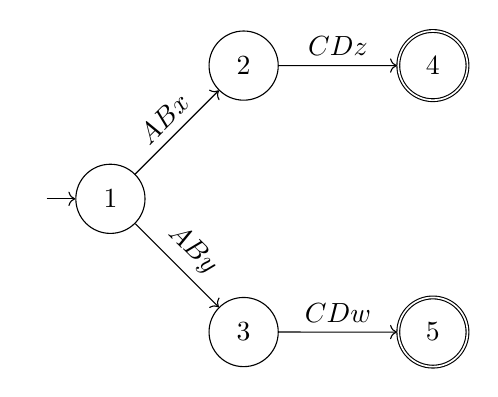
\begin{tikzpicture}[node distance=1.5cm, auto, scale=0.8]
		\node[state, initial, initial text={}] (s0) {1};
		\node[state] (s1) [above right=of s0] {2};
		\node[state] (s2) [below right=of s0] {3};
		\node[state,accepting] (s3) [right=of s1] {4};
		\node[state,accepting] (s4) [right=of s2] {5};

		\draw[->] (s0) to node[above,sloped]{$\gtlabel{A}{B}{x}$}(s1);
		\draw[->] (s0) to node[above,sloped]{$\gtlabel{A}{B}{y}$}(s2);
		\draw[->] (s1) to node[above,sloped]{$\gtlabel{C}{D}{z}$}(s3);
		\draw[->] (s2) to node[above,sloped]{$\gtlabel{C}{D}{w}$}(s4);
	\end{tikzpicture}
	\caption{An automaton representing the specification's global type given in Listing~\ref{lst:not-impl-exm}.}
	\label{fig:gt-exm}
\end{figure}
\end{example}

\bigskip

% --------------relationship between MSCs and Global Types--------------

We can now formally define the relationship between MSCs and Global Types. 
Intuitively, Global Types represent a set of MSCs, allowing us to reason 
about multiple message sequence scenarios. 

A Global Type defines a language of MSCs in two different ways, one
existential and one universal. Let $\labellanguageof{\gt}$ be the set of
sequences of arrows $w$ accepted by $\gt$.
Informally, the existential MSC language $\existentialmsclanguageof{\gt}{}$ of a 
Global Type $\gt$ is the set of MSCs that admit at least one representation as a
sequence of arrows in $\labellanguageof{\gt}$, and the universal MSC
language $\universalmsclanguageof{\gt}$ of a Global Type $\gt$ is the set of
MSCs whose representations as sequences of arrows are all in
$\labellanguageof{\gt}$. We will just give the formal definition of
$\existentialmsclanguageof{\gt}{}$:

\bigskip

\begin{definition}[$\existentialmsclanguageof{\gt}$]
	$$
		\existentialmsclanguageof{\gt} \eqdef \{\labeltomsc{w} \mid
		w \in \labellanguageof{\gt}\}
  	$$
\end{definition}

% TODO: dare più contesto ed esempio

When a global type is implemented in a concrete system,
its behaviour depends on the chosen communication model.

\bigskip

\begin{definition}[Global Type Language]\label{def:global-type-language}
    Let $\gt$ be a global type and $\acommunicationmodel$ a communication model. 
    The language of $\gt$ in $\acommunicationmodel$ is $
    \executionsof{\gt}{\acommunicationmodel}\eqdef
    \bigcup\{\linearizationsof{M}{\acommunicationmodel}\mid M\in\existentialmsclanguageof{\gt}\}$.
\end{definition}

% TODO: FARE UN CONFRONTO CON LE DUE DEFINIZIONI
We now give the definitions of weak and safe realisability.

\bigskip

\begin{definition}[Weak realisability]\label{def:gt-weak-realis}
A global type $\gt$ is \emph{weak realisable} in the
communication model $\acommunicationmodel$ if there is a
system CFSM $\cfsms$ such that the following condition hold:
$\executionsof{\cfsms}{\acommunicationmodel} =
\executionsof{\gt}{\acommunicationmodel}$.
\end{definition}

Although this work does not focus on safe realisability, we will still
define it formally to highlight the main differences and similarities 
with other works in Chapter~\ref{sec:rel}.

\bigskip

\begin{definition}[Safe realisability]\label{def:gt-safe-realis}
    A global type $\gt$ is \emph{safe realisable}
    in the communication model $\acommunicationmodel$
    if there is a system $\cfsms$ that is \emph{weak realisable} and  
    $\cfsms$ is deadlock-free in $\acommunicationmodel$.
\end{definition}

The definition of Weak realisability corresponds to  
the property of \emph{global type conformance}: all system executions 
faithfully follow the behaviours prescribed by the global type.
When $\acommunicationmodel$ is $\ppmodel$ or $\synchmodel$, 
our notion of safe realisability coincides with the notion of 
\emph{safe realisability} introduced in~\cite{alur2005realizability}.
This equivalence does not extend to more general communication models, 
such as the mailbox model~\cite{di2025realisability}.
% TODO: come dare supporto a queste affermazioni?
We are now ready to present the main contributions of this work.

\chapter{Weak-Realisability is Undecidable for Synchronous Global Types}
\label{sec:proof}

This chapter presents the first main contribution of this thesis, formalised in
Theorem~\ref{thm:main}, which establishes that 
\emph{Weak-realisability is undecidable for synchronous global types}.  
This result complements the broader reduction theorem introduced in
Section~\ref{sec:red}, where we showed how the realisability problem for
peer-to-peer systems can be reduced to the study of realisability under
synchronous semantics.  
Here, we focus exclusively on this synchronous setting, proving that even in such
a constrained communication model, weak realisability remains undecidable.

To support this proof, Chapter~\ref{sec:pre} introduced the necessary background on
Message Sequence Charts (MSCs), Global Types, and Weak-realisability.  
In this chapter, we build upon those foundations by formally defining the
core constructions used in the proof of Theorem~\ref{thm:main}.  
The proof itself is inspired by the classical reduction of 
Alur et~al.~\cite{alur2005realizability}, which we extend and adapt to the
framework of synchronous global types.  
Along the way, we emphasise the main conceptual and technical differences
between our approach and the original construction, clarifying how these 
adaptations enable the result to hold in the synchronous semantic setting.

\section{Definitions}
The proof is a \emph{reduction} from the
\textbf{Relaxed Post Correspondence Problem (RPCP)}, a variant of
the classical Post Correspondence Problem (PCP). 
RPCP was shown to be undecidable by
Alur~et~al.~\cite{alur2005realizability}, via reduction from PCP.
The main idea is to encode the existence of a
solution to an RPCP instance into the non-realisability of our formal
specification. In the original proof, MSCs are directly used to build an
HMSC called $M^*$. In our case, we will define a
\emph{global type} (called $L^*$) built from global types.
A generic solution for the RPCP problem will correspond to the global
type $L^*$. Therefore, we need to prove:
$$
\Delta \in \text{RPCP} \quad\iff\quad L^* \text{ is not realisable}.
$$

\bigskip

\begin{definition}[Relaxed Post Correspondence Problem]
	Given a set of tiles $\{(v_1, w_1), (v_2, w_2), ..., (v_r, w_r)\}$, 
	determining whether there exist indices $i_1, ..., i_m$ such that
	$$x_{i_1}\cdots x_{i_m} = y_{i_1}\cdots y_{i_m},$$
	where $x_{i_j}, y_{i_j} \in \{v_{i_j}, w_{i_j}\}$, such that:
	\begin{itemize}
		\item there exists at least one index $i_\ell$ for which $x_{i_\ell}\neq y_{i_\ell}$, and
		\item for all $j \leq m$, $y_{i_1}\cdots y_{i_j}$ is a strict or 
		not-strict prefix of $x_{i_1}\cdots x_{i_j}$.
	\end{itemize}
\end{definition}

Intuitively, RPCP requires that the concatenation on the left-hand side always 
grows at least as fast as the right-hand side, while ensuring that at least one 
chosen tile differs between the two sequences. Moreover, in constructing the 
strings, we may freely choose which element of each tile (either $v_i$ or $w_i$) 
contributes to the left or right sequence.

\bigskip

\begin{example}[Simple RPCP instance]\label{exmp:rpcp}
Consider the tile set
\[
(v_1,w_1)=(\texttt{b},\ \texttt{bb}),\quad
(v_2,w_2)=(\texttt{a},\ \texttt{ab}),\quad
(v_3,w_3)=(\texttt{c},\ \texttt{c}).
\]
Take the index sequence $(2,1,3)$ and the choices
\[
x_1 = w_2,\ y_1 = v_2;\quad
x_2 = v_1,\ y_2 = w_1;\quad
x_3 = v_3,\ y_3 = w_3.
\]
Then
\[
x_1 x_2 x_3 = \texttt{ab}\ \texttt{b}\ \texttt{c} = \texttt{abbc},
\qquad
y_1 y_2 y_3 = \texttt{a}\ \texttt{bb}\ \texttt{c} = \texttt{abbc},
\]
so the two sides are equal.

We now check the RPCP conditions:
\begin{itemize}
  \item \textbf{at least one mismatch:} here $x_1\neq y_1$ and
        $x_2\neq y_2$, so the ``some index differs'' condition holds;
  \item \textbf{prefix property:} for every prefix length $j$ we have
        $y_{1}\cdots y_{j}$ is a prefix of $x_{1}\cdots x_{j}$:
        \begin{itemize}
          \item $j=1$: $y_1=\texttt{a}$ is a prefix of $x_1=\texttt{ab}$;
          \item $j=2$: $y_1y_2=\texttt{abb}$ is a prefix of $x_1x_2=\texttt{abb}$;
          \item $j=3$: $y_1y_2y_3=\texttt{abbc}$ is a prefix of $x_1x_2x_3=\texttt{abbc}$.
        \end{itemize}
\end{itemize}
\end{example}

\bigskip

We have now identified the main problem to which our proof reduces.  
The next step is to encode an RPCP instance into the formal model.
In the original proof, MSCs are used, but, in our case, we also need to give
an encoding using Global Types. We will first give the MSC one.

\bigskip

\begin{definition}[$M^n_i$]\label{def:mni}
	Given the index $i$ of a tile $(v_i, w_i)$, and
	given an interger $n\in\{0,1\}$, where:
	\begin{itemize}
		\item if $n=0$, then $x_i=v_i$;
		\item if $n=1$, then $x_i=w_i$;
	\end{itemize}
	The behavior of the MSC $M^n_i$ is as follows:
	first, Process~1 synchronously sends message
	$m_1 = (i, n)$ to Process~2, then Process~1 transmits the index $m_2=i$
	to Process~4. Subsequently, Process~4 sends $m_3 = (i, n)$
	synchronously to Process~3. After these control messages, Process~2
	sends the characters $m_i^1 = x_i^1,..., m_i^c = x_i^c$
	synchronously to Process~3 (where $c$ is the length of $x_i$).
	This MSC is depicted in Figure~\ref{fig:mni}, 

	\begin{figure}[!ht]
		\centering
		\begin{msc}[draw frame=none, draw head=none, msc keyword=, head height=0px, label distance=0.5ex, foot height=0px, foot distance=0px]{}
			\declinst{P1}{P1}{}
			\declinst{P2}{P2}{}
			\declinst{P3}{P3}{}
			\declinst{P4}{P4}{}

			\syncmscmess{$(i,n)$}{P1}{P2}
			\syncmscmess{$i$}{P1}{P4}
			\syncmscmess{$(i,n)$}{P4}{P3}
			\syncmscmess{$x_i^1$}{P2}{P3}
			\syncmscmess{...}{P2}{P3}
			\syncmscmess{$x_i^c$}{P2}{P3}
		\end{msc}
		\caption{The $M_i^n$ MSC.}
		\label{fig:mni}
	\end{figure}

\end{definition}

Given a RPCP instance $\{(v_1,w_1),\ldots,(v_m,w_m)\}$, we associate  
with each pair $(v_i,w_i)$ two MSCs $M^0_i$ and $M^1_i$, following  
Definition~\ref{def:mni}. Each MSC $M^n_i$ is \emph{synchronous}  
(Lemma~\ref{lemma:minsynch}). Intuitively, the MSC $M_i^n$ encodes the  
construction of a string given some tiles through the interaction of four processes.  
Processes~2 and~3 are responsible for building the string itself,  
while Processes~1 and~4 transmit the index information to Processes~2  
and~3, respectively. In particular, Process~1 initiates the choice and  
forwards it to Process~4. This encoding applies equally to definition~\ref{def:gni}.

\bigskip

\begin{lemma}\label{lemma:minsynch}
The MSC $M_i^n$ belongs to $\mscsetofmodel{\synchmodel}$.
\end{lemma}

\begin{proof}
By Definition~\ref{def:msc}, each communication in $M_i^n$
consists of a send event $\send{p}{q}{m}$ and its corresponding
receive event $\recv{p}{q}{m}$, with $\source(\recv{p}{q}{m}) =
\send{p}{q}{m}$.  
By Definition~\ref{def:synchronous}, an MSC is synchronous
if there exists a linearisation in which every send event
immediately precedes its matching receive.

In $M_i^n$, the set of messages exchanged is
\[
\{\, m_1, m_2, m_3, m_i^1, \ldots, m_i^c \,\},
\]
with $c = |x_i|$.  
A valid synchronous linearisation therefore exists and is given by:
\[
!m_1 ?m_1\;\; !m_2 ?m_2\;\; !m_3 ?m_3\;\;
!m_i^1 ?m_i^1 \;\ldots\; !m_i^c ?m_i^c.
\]
This linearisation satisfies the synchronous ordering constraint,
as every send is immediately followed by its matching receive.
Hence, by Definition~\ref{def:linearisable-msc},  
$M_i^n \in \mscsetofmodel{\synchmodel}$.
\end{proof}

We now define how to obtain a Global Type on top of an MSC.

\bigskip

\begin{definition}[$\gt_M$]\label{def:gm}
Let $M \in \mscsetofmodel{\synchmodel}$ be a message sequence chart (MSC)  
over the set of processes $\Procs$ and messages $\Messages$.  
We construct the corresponding Global Type $\gt_M = (Q, \Sigma, \delta, q_0, F)$  
as follows.

\begin{itemize}

    \item
    The alphabet $\Sigma$ is the set of \emph{synchronous communication arrows}  
    \[
        \Sigma = \{\, \marrow{p}{q}{m} \mid 
        \exists \, \event_s \in \sendeventsof{M}, \, 
        \event_r \in \receiveeventsof{M} \text{ such that }
	\]
    \[
        \source(\event_r) = \event_s, \, 
        \processof{\event_s}=p, \, \processof{\event_r}=q, \, 
        \messageof{\event_s}=m \,\}.
    \]

    \item
    Since $M \in \mscsetofmodel{\synchmodel}$, there exists a  
    \emph{synchronous linearisation}  
    $w = \alpha_1 \alpha_2 \ldots \alpha_k$,  
    where each $\alpha_j = \marrow{p_j}{q_j}{m_j} \in \Sigma$  
    represents a complete synchronous communication step (send immediately  
    followed by its matching receive).

    \item
    Let $Q = \{ q_0, q_1, \ldots, q_k \}$,  
    where $q_0$ is the initial state and $q_k$ is the unique accepting state.

    \item
    The transition function $\delta : Q \times \Sigma \to Q$  
    is defined sequentially along the synchronous interactions of $M$:  
    \[
        \forall j \in \{1, \ldots, k\}, \quad  
        \delta(q_{j-1}, \alpha_j) = q_j.
    \]
    All other transitions are undefined.

\end{itemize}

\end{definition}

Intuitively, $\gt_M$ captures the exact synchronous execution order of $M$:  
it is the deterministic automaton that accepts the single word  
$w = \alpha_1 \alpha_2 \ldots \alpha_k$ over $\Sigma$,  
representing the sequence of message exchanges in $M$.  
Equivalently, $\gt_M$ recognises the set of MSCs whose synchronous  
linearisations are $w$.
We now use this definition to encode $M_i^n$ in a Global Type format.

\bigskip

\begin{definition}[$G_i^n$]\label{def:gni}
Let $(v_i, w_i)$ be a tile and $n \in \{0,1\}$.  
Set $x_i = v_i$ if $n = 0$, and $x_i = w_i$ if $n = 1$.  
Let $c = |x_i|$ and write $x_i = x_i^1 x_i^2 \cdots x_i^c$.

The global type $G_i^n$ (shown in Figure~\ref{fig:gni}) is the DFA
$G_i^n = (Q, \Sigma, \delta, q_0, F)$, obtained
on top of the MSC $M_i^n$ (Definition~\ref{def:mni}) using the 
construction in Definition~\ref{def:gm}, and defined as follows:
\begin{itemize}
	\item $\mathbb{P} = \{P1, P2, P3, P4\}$;
	\item $\mathbb{M} = \{m_1, m_2, m_3, m_{x_i^1}, \ldots, m_{x_i^c}\}$,
	      where $m_1 = (i, n)$, $m_2 = i$, $m_3 = (i, n)$, and
	      $m_{x_i^j} = x_i^j$ for $1 \le j \le c$;
	\item $\text{Arr} = \{\,$\arrmess{P1}{P2}{m_1}$,\, $\arrmess{P1}{P4}{m_2}$,\,
	      $\arrmess{P4}{P3}{m_3}$,\, $\arrmess{P2}{P3}{m_{x_i^1}}$, \ldots,
	      $\arrmess{P2}{P3}{m_{x_i^c}}$\,\}$, where each arrow denotes
	      a synchronous message with acknowledgment;
	\item $Q = \{q_0, q_1, q_2, q_3, q_4, \ldots, q_{3+c}\}$,  
	      where $q_0$ is the initial state and  
	      $F = \{q_{3+c}\}$ is the unique accepting state;
	\item The alphabet $\Sigma$ is the finite set of arrows (synchronous message labels):  
	      $
	      \Sigma = 
	      \{\,$\arrmess{P1}{P2}{m_1}$,\,
	           $\arrmess{P1}{P4}{m_2}$,\,
	           $\arrmess{P4}{P3}{m_3}$\,\}
	      \cup
	      \{\,$\arrmess{P2}{P3}{m_{x_i^j}}$ \mid 1 \le j \le c\,\}.
	      $
	\item The (deterministic) transition function
	      $\delta : Q \times \Sigma \to Q$ is defined by:
	        $  \delta(q_0,\, $\arrmess{P1}{P2}{m_1}$) = q_1,\ 
	          \delta(q_1,\, $\arrmess{P1}{P4}{m_2}$) = q_2, \ 
	          \delta(q_2,\, $\arrmess{P4}{P3}{m_3}$) = q_3, \ 
	          \delta(q_{2+j},\, $\arrmess{P2}{P3}{m_{x_i^{j+1}}}$) = q_{3+j}, 
	          \  0 \le j < c.$
	      Hence, the sequence of transitions from $q_3$ to $q_{3+c}$ 
	      corresponds to the synchronous exchanges between $q$ and $r$
	      labelled by $m_{x_i^1}, \ldots, m_{x_i^c}$.
\end{itemize}

	\begin{figure}[!ht]
		\centering
		\begin{tikzpicture}[->, node distance=35mm, on grid, auto]
			\node[state] (q0) {$q_0$};
			\node[state] (q1) [right=of q0] {$q_1$};
			\node[state] (q2) [right=of q1] {$q_2$};
			\node[state] (q3) [below left=of q0] {$q_3$};
			\node[state] (q4) [right=of q3] {$q_4$};
			\node[state] (q5) [right=of q4] {$\cdots$};
			\node[state,accepting] (q6) [right=of q5] {$q_x$};

			\path (q0) edge[] node[above] {\arrmess{P1}{P2}{(i,n)}} (q1);
			\path (q1) edge[] node[above] {\arrmess{P1}{P4}{i}} (q2);
			\path (q2) edge[] node[above left] {\arrmess{P4}{P3}{(i,n)}} (q3.60);
			\path (q3) edge[] node[above] {\arrmess{P2}{P3}{x_i^1}} (q4);
			\path (q4) edge[] node[above] {\arrmess{P2}{P3}{...}} (q5);
			\path (q5) edge[] node[above] {\arrmess{P2}{P3}{x_i^c}} (q6);
		\end{tikzpicture}
		\caption{The global type $G_i^n$.}
		\label{fig:gni}
	\end{figure}

\end{definition}

% Intuitively, $G_i^n$ specifies the same communication pattern as the MSC  
% $M^n_i$ introduced in Definition~\ref{def:mni}. This structural  
% correspondence will be made precise in the next lemma (Lemma~\ref{lem:gm}).  

Intuitively, using the costruction defined in Definition~\ref{def:gm},
we obtain a Global Type whose existential language of representation
correspond exactly to the given MSC. 

\bigskip

\begin{lemma}\label{lem:gm}
For every MSC $M \in \mscsetofmodel{\synchmodel}$,  
there exists a Global Type $\gt_M$ such that  
$\existentialmsclanguageof{\gt_M} = \{ M \}$.
\end{lemma}

\begin{proof}
Let $M \in \mscsetofmodel{\synchmodel}$ and let $\gt_M$ be the Global Type  
constructed as in Definition~\ref{def:gm}.  
By definition, $\gt_M$ is the DFA that accepts exactly  
the synchronous linearisation  
$w = \alpha_1 \alpha_2 \ldots \alpha_k$ of $M$,  
where each $\alpha_j = \marrow{p_j}{q_j}{m_j}$  
corresponds to a complete synchronous communication.  
Since every execution of $\gt_M$ under the synchronous semantics  
follows the exact sequence of communications in $w$,  
it induces the same causal and message relations as in $M$.  
Hence, the unique MSC corresponding to any accepting run of $\gt_M$  
is precisely $M$.  
Conversely, any MSC $M'$ whose synchronous linearisation is accepted  
by $\gt_M$ must have the same sequence of synchronous interactions as $M$,  
and therefore $M' = M$.  
Therefore, the existential MSC-language of $\gt_M$ contains exactly $M$,  
that is,
\[
    \existentialmsclanguageof{\gt_M} = \{ M \}.
\]
\end{proof}


Lemma~\ref{lem:gm} establishes a direct correspondence between a  
single synchronous MSC and a Global Type. In particular, every  
synchroonus MSC can be captured precisely by a Global Type whose  
language contains only that MSC. This correspondence will be useful  
when embedding RPCP instances into the Global Type framework.
We now introduce a more structured Global Type, parameterized by a  
string $S$, which will serve as the building block in the reduction.

Thanks to Lemma~\ref{lem:gm} and given that $M_i^n$
is a synchronous MSC (Lemma~\ref{lemma:minsynch}), 
we can establish now that 
$\existentialmsclanguageof{G_i^n} =\{M_i^n\}$.
After establishing the connection between the MSC's encoding and
Global Type's encoding,
we briefly summarize the rationale behind the design of $M_i^n$ and $G_i^n$.

Suppose that $\Delta=(i_1,a_1,b_1,\ldots,i_m,a_m,b_m)$ is a  
solution to the RPCP instance. From this solution we construct   
two MSCs sequences:
\[
M_x = M^{a_1}_{i_1}\cdots M^{a_m}_{i_m}, \qquad  
M_y = M^{b_1}_{i_1}\cdots M^{b_m}_{i_m}.
\]
Both $M_x$ and $M_y$ are concatenations of synchronous  
MSCs. We then define a third MSC $M_{\texttt{sol}}$, obtained by  
projecting $M_y$ onto processes $P1,P2$ and $M_x$ onto processes  
$P3,P4$. Intuitively, processes $P1,P2$ represent the construction of  
the \emph{right-hand string} $y_{i_1}\cdots y_{i_m}$, while processes  
$P3,P4$ represent the construction of the \emph{left-hand string}  
$x_{i_1}\cdots x_{i_m}$. The prefix property of RPCP guarantees that  
$M_{\texttt{sol}}$ is acyclic and \emph{synchronous}. Establishing that 
$M_{\texttt{sol}} \in \mscsetofmodel{\synchmodel}$ is non-trivial, and this 
step is an addition to the original proof. 

% With these constructions in place, we proceed to introduce the main  
% objects used in the proof. Specifically, we first show how a Global  
% Type can represent a single \verb|synch| MSC.

% \bigskip

% \begin{lemma}\label{lmm:msgs}
% Assume $\acommunicationmodel$ is the $\synchmodel$ model and $i,n$ are integers.
% The MSC $M^n_i$ (Definition~\ref{def:mni}) is included in 
% $\msclanguageof{G_i^n}{\synchmodel}$ (Definition~\ref{def:gni}).
% \end{lemma}

% % TODO: Da rifare meglio, non ha senso quel L(M) = L(G)
% \begin{proof}
% 	Both $M^n_i$ and $G_i^n$ describe the same communication structure:
% 	process $p$ sends $(i,n)$ to $q$ and $i$ to $s$;
% 	process $s$ relays $(i,n)$ to $r$;
% 	process $q$ then sends the characters of $x_i$ to $r$.
% 	The sequence of messages is identical in both 
% 	$M^n_i$ and $G_i^n$. Since both models enforce synchronous communication, 
% 	their linearisations coincide. 
% 	Hence, $M^n_i \in \msclanguageof{G_i^n}{\synchmodel}$.
% \end{proof}

% Having established the correspondence between an individual MSC and its
% associated global type, we now extend this construction to sets of global
% types. 
The following definition introduces the global type $L^*$, which
encapsulates all possible compositions derived from a given RPCP instance.
Intuitively, for each MSC $M \in \setmsc$, there exists a corresponding
global type $G \in G^*$ that captures the behaviour described by $M$.
The automaton defining $L^*_N$ then combines all such global types in $G^*$
into a single structure, allowing transitions between them through
$\varepsilon$-moves. The determinisation of this automaton yields the
global type $L^*$, representing the full set of possible interactions
generated by the collection of MSCs.

\bigskip

\begin{definition}[The $L^*$ global type]\label{def:lstar}
	Given an instance $\{(v_1, w_1), \ldots, (v_m, w_m)\}$ of RPCP, we
	construct a set $M^* = \{M_i^0, M_i^1 \mid i \in \{1, \ldots, m\}\}$ of
	MSCs over four processes as follows. For each pair $(v_i, w_i)$,
	we define two MSC, $M_i^0$ and $M_i^1$, as specified in
	Definition~\ref{def:mni} and illustrated in Figure~\ref{fig:mni}.
	For each MSC in $M^*$, we construct $G^*$ using Definition~\ref{def:gm}.
	Every Global Type in $G^*$ is shaped like Definition~\ref{def:gni} 
	(shown in Figure~\ref{fig:gni}).
	We define the global type $L^*_{N}$ as the automaton
	$\mathcal A = (Q,\Sigma, \delta, l_0, F)$ where:
	\begin{itemize}
		\item $Q = \{v_I,v_T\}\cup \bigcup_{G\in G^*} Q^G$;
		\item $\Sigma = \{\epsilon\}\cup\bigcup_{G\in G^*} \Sigma^G$;
		\item $\delta: Q \times \Sigma \rightarrow 2^Q$ is defined by:
			      \begin{enumerate}
				       \item $\forall G \in G^*,\ \delta(v_I, \varepsilon) = q_0^G$ where $q_0^G$ is the initial state of $G$,
				       \item $\forall G \in G^*,\ \forall q_f^G \in F^G,\ \delta(q_f^G, \varepsilon) = v_T$,
				       \item $\forall G, G' \in G^*,\ \forall q_f^G \in F^G,\ \delta(q_f^G, \varepsilon) = q_0^{G'}$.
			      \end{enumerate}
		\item $l_0 = v_I$ is the initial state;
		\item $F = v_T$ is the accepting state.
	\end{itemize}
	The automaton of $L^*_{N}$ is shown in Figure~\ref{fig:lstar}.  
	Finally, the Global Type $L^*$ is obtained as the determinisation 
	of $L^*_{N}$ (Definition~\ref{def:det}).
\end{definition}

\begin{figure}[!ht]
	\centering
	\begin{tikzpicture}[->, node distance=35mm, on grid, auto]
		\node[state] (vI) {$v_I$};
		\node[state] (qI2) [right=of vI] {$\cdots$};
		\node[state] (qI1) [above=of qI2] {$q_0^{G^1}$};
		\node[state] (qI3) [below=of qI2] {$q_0^{G^n}$};
		\node[state] (qM1) [right=of qI1] {$\cdots$};
		\node[state] (qM2) [right=of qI2] {$\cdots$};
		\node[state] (qM3) [right=of qI3] {$\cdots$};
		\node[state] (qF1) [right=of qM1] {$q_f^{G^1}$};
		\node[state] (qF2) [right=of qM2] {$\cdots$};
		\node[state] (qF3) [right=of qM3] {$q_f^{G^n}$};
		\node[state,accepting] (vT) [right=of qF2] {$v_T$};

		\path (vI) edge[] node[above] {$\epsilon$} (qI1);
		\path (vI) edge[] node[above] {$\epsilon$} (qI2);
		\path (vI) edge[] node[above] {$\epsilon$} (qI3);
		\path (qI1) edge[] node[above] {\arrmess{p}{q}{(i^{G^1},n^{G^1})}} (qM1);
		\path (qI2) edge[] node[above] {} (qM2);
		\path (qI3) edge[] node[above] {\arrmess{p}{q}{(i^{G^n},n^{G^n})}} (qM3);
		\path (qM1) edge[] node[above] {\arrmess{q}{r}{x^{G^1}_c}} (qF1);
		\path (qM2) edge[] node[above] {} (qF2);
		\path (qM3) edge[] node[above] {\arrmess{q}{r}{x^{G^n}_c}} (qF3);
		\path (qF1) edge[] node[above] {$\epsilon$} (vT);
		\path (qF2) edge[] node[above] {$\epsilon$} (vT);
		\path (qF3) edge[] node[above] {$\epsilon$} (vT);
		
		\draw (qF1.135) to [bend right=30] node[above] {$\epsilon$} (qI1.45);
		\draw (qF2.135) to [bend right=30] node[above] {$\epsilon$} (qI2.45);
		\draw (qF3.135) to [bend right=30] node[above] {$\epsilon$} (qI3.45);

		\draw (qF1.225) to node[above] {$\epsilon$} (qI2.60);
		\draw (qF3.120) to node[above] {$\epsilon$} (qI2.315);
		
		\draw (qF3) .. controls +(8,10) and +(1,3) .. node[midway,above] {$\epsilon$} (qI1);
		\draw (qF1) ..  controls +(8,-10) and +(1,-3) .. node[midway,above] {$\epsilon$} (qI3);
	\end{tikzpicture}
	\caption{The automaton of the global type $L^*_N$.}
	\label{fig:lstar}
\end{figure}

In other words, $L^*$ is a Global Type whose language of executions
captures all possible combinations and exchanges of choices arising in a
generic instance of the RPCP problem.
This global type is constructed from the family of global types % TODO: forse cambiare in MSC
representing all tiles, and it forms the basis for proving the
non-realisability result.

Given the system of CFSMs $\projectionof{L^*}$ and the MSC  
$M_{\texttt{sol}}$, we need to show that  
$\executionsof{\projectionof{L^*}}{\synchmodel} \neq \executionsof{L^*}{\synchmodel}$.  
By construction of $L^*$, we have  
$M_{\texttt{sol}} \in \msclanguageof{\projectionof{L^*}}{\synchmodel}$.  
In contrast, $M_{\texttt{sol}} \notin  
\msclanguageof{L^*}{\synchmodel}$, since at least one tile differs.  
This demonstrates that there exists an execution that is valid for  
$\projectionof{L^*}$ but invalid for the Global Type $L^*$.  
Therefore, $L^*$ is \emph{not realisable}.  


\section{Undecidability proof}

Given the definitions and lemmas stated in the last section, we are now ready
to present the proof for the undecidability result.

\bigskip

\begin{theorem}\label{thm:main}
	Given a global type $G$, checking if $G$ is weakly-realisable is undecidable.
\end{theorem}

\begin{proof}
	The proof proceeds via a reduction from the RPCP problem.
	Given an instance $\{(v_1, w_1), \ldots, (v_m, w_m)\}$ of RPCP, we
	construct $L^*$ as specified in Definition~\ref{def:lstar}.
	
	We need to prove:
	\begin{center}
		$\Delta \in \text{RPCP}$ iff the global type $L^*$ is not weakly-realisable.
	\end{center}

	\begin{itemize}
		\item[$\Rightarrow$]
			Assume that
			$\Delta = (i_1, a_1, b_1, i_2, a_2, b_2, \ldots, i_m, a_m, b_m)$ are the indices
			for a solution to a generic RPCP problem instance, and the bits $a_j$ and
			$b_j$ indicate which string ($v_{i_j}$ or $w_{i_j}$) is chosen to go into
			the two (left and right) long strings. Assume also synchronous communication semantic.
			Consider the MSCs $M_x$ and $M_y$ obtained from the concatenation of
			$M_x = M^{a_1}_{i_1} \cdots M^{a_m}_{i_m}$ 
			and $M_y = M^{b_1}_{i_1} \cdots M^{b_m}_{i_m}$.
			The possible linearisations of both of these sequences of MSCs 
			must be included in the language of execution of $L^*$, by construction 
			of $L^*$ (Definition~\ref{def:lstar}). 
			This means that $M_x, M_y \in \msclanguageof{L^*}{\synchmodel}$.
			Additionally, $M_x,M_y\in \mscsetofmodel{\synchmodel}$
			because they are sequences of MSCs included in
			$\mscsetofmodel{\synchmodel}$ (Lemma~\ref{lemma:minsynch}).
			$M_x$ corresponds to the construction of the left side of the equivalence of the RPCP
			problem, and, instead, $M_y$ represents the construction of the right side.
			We then look at the projections $M_x|_{P1}$, $M_x|_{P2}$, $M_x|_{P3}$,
			and $M_x|_{P4}$ of $M_x$, and $M_y|_{P1}$, $M_y|_{P2}$, $M_y|_{P3}$, $M_y|_{P4}$ of $M_y$ onto the
			4 processes.
			Given that these are projection of MSCs included in $L^*$,
			they are possible execution of a CFSM $\cfsms$ that can execute $L^*$.
			Now consider the MSC $M_{\texttt{sol}}$ 
			formed from $M_y|_{P1}$, $M_y|_{P2}$, $M_x|_{P3}$, and $M_x|_{P4}$.
			This MSC represents the construction of the solution to
			the problem. Processes 1 and 2 construct the right part ($y_{i_1}...y_{i_m}$)
			and processes 3 and 4 construct the left part ($x_{i_1}...x_{i_m}$).
			%%% INIZIO PARTE IMPORTANTE
			The claim is that the combined MSC $M_{\texttt{sol}}$ is 
			made by $L^*$'s projections, therefore, it exists a CFSM $\cfsms$
			that $M_{\texttt{sol}} \in \mscsofcfsms{\cfsms}{\synchmodel}$,
			but the CFSM $\cfsms$ is not part of the language of execution of $L^*$ 
			$\executionsof{\cfsms}{\synchmodel} \neq \executionsof{L^*}{\synchmodel}$. 
			In other words, the language of the execution of $M_{\texttt{sol}}$ is included
			in the execution of the system, but it is not included in the execution of $L^*$. 
			By definition, the first thing to establish is that $M_{\texttt{sol}}$
			is indeed well-formed and synchronous MSC.
			The only new situation in terms of communication in $M_{\texttt{sol}}$ is the
			communication between $P_1$ and $P_4$, and between $P_2$ and $P_3$.
			But the communication between $P_1$ and $P_4$ is consistent in
			$M_y|_{P1}$ and $M_x|_{P4}$ (i.e., the sequence of messages sent from $P_1$ to
			$P_4$ in $M_y|_{P1}$ is equal to the sequence of messages received in $M_x|_{P4}$),
			and the communication between $P_2$ and $P_3$ is consistent in
			$M_y|_{P2}$ and $M_x|_{P3}$ because $R$ is a solution to the RPCP.
			Furthermore, the acyclicity of $M_{\texttt{sol}}$ follows from the property of the
			solution that the string formed by the first $j$ words on processes 1
			and 2 is always a prefix of the string formed by the first $j$ words
			on processes 3 and 4. Consequently, each message from $P_1$ to $P_4$
			is sent before it needs to be received. 
			Therefore, the MSC $M_{\texttt{sol}}$ is well-formed.

			We now prove that the MSC $M_{\texttt{sol}}$ is synchronous, that is
			$M_{\texttt{sol}} \in \mscsetofmodel{\synchmodel}$.
			Assume, by contradiction, that 
			$M_{\texttt{sol}} \notin \mscsetofmodel{\synchmodel}$.
			Then, there should be a cycle of dependencies in the communication pattern.
			There are no communication between $P_2$ and $P_4$, and between $P_1$
			and $P_3$. Therefore, this cycle must involve all processes, starting
			for example from $P_1$ and having this dependency graph
			$P_1\leftrightarrow P_2\leftrightarrow P_3\leftrightarrow P_4\leftrightarrow P_1$.
			The only new situation that can cause a cycle are the communication
			between $P_1$ and $P_4$, and between $P_2$ and $P_3$.
			We do not need to analyse the new communication between $P_1$ and $P_4$ because
			it is not feasible in any communication model, but we need to analyse the one
			between $P_2$ and $P_3$ because it's feasible in FIFO.

			% For the fist comunication, the only possible cycle pattern is depicted
			% in Fig.~\ref{fig:cycle1}

			% \begin{figure}[!ht]
			%  \centering
			%  \begin{msc}[draw frame=none, draw head=none, msc keyword=, head height=0px, label distance=0.5ex, foot height=0px, foot distance=0px]{}
			%   \declinst{P1}{P1}{}
			%   \declinst{P2}{P2}{}
			%   \declinst{P3}{P3}{}
			%   \declinst{P4}{P4}{}

			%   \mess[label position=above right,pos=0.45]{$i_z$}{P1}{P4}[8]
			%   \nextlevel
			%   \nextlevel
			%   \nextlevel
			%   \syncmscmess{($i_k,n_k)$}{P1}{P2}
			%   \mess[label position=above,pos=0.62]{$i_k$}{P1}{P4}
			%   \mess{}{P4}{P1}
			%   \nextlevel
			%   \syncmscmess{$(i_k,n_j)$}{P3}{P4}
			%   \nextlevel
			%   \nextlevel
			%   \mess{}{P4}{P1}[-8]
			%  \end{msc}
			%  \caption{The $M_i^n$ MSC.}
			%  \label{fig:cycle1}
			% \end{figure}

			% This cycle is not possible because it does not represent a
			% solution to the RPCP problem:
			% $x_1...x_{i_k}...x_{i_z}...x_m \neq y_1...y_{i_z}...y_{i_k}...y_m$.

			\begin{figure}[!ht]
				\centering
				\begin{msc}[draw frame=none, draw head=none, msc keyword=, head height=0px, label distance=0.5ex, foot height=0px, foot distance=0px]{}
					\declinst{P1}{P1}{}
					\declinst{P2}{P2}{}
					\declinst{P3}{P3}{}
					\declinst{P4}{P4}{}

					\mess[label position=above right, pos=0.3]{$c$}{P2}{P3}[4]%
					\nextlevel
					\syncmscmess{$(i_k,n_k)$}{P1}{P2}
					\mess[pos=0.62]{$i_k$}{P1}{P4}%
					\mess{}{P4}{P1}
					\nextlevel
					\syncmscmess{$(i_k,n_j)$}{P3}{P4}
					\mess{}{P3}{P2}[-4]
				\end{msc}
				\caption{MSC communication that breaks synchrony.} % todo: modifica
				\label{fig:cycle2}
			\end{figure}

			For the communication between $P_2$ and $P_3$, the only possible cycle
			pattern is depicted in Figure~\ref{fig:cycle2} showed as an MSC.
			Suppose $P_2$ wants to send a character $c$, but $P_3$
			is not expecting any further characters. In order for
			$P_3$ to resume receiving, it must first receive an index
			from $P_4$. However, $P_4$ can only send this index
			after receiving it from $P_1$, which in turn must first
			communicate the index to $P_2$.
			At this point, $P_2$ needs to receive the index from
			$P_1$, but it cannot do so until it finishes sending
			character $c$. This creates a circular dependency among the
			processes, making the communication pattern impossible. % TODO: chiarire che non è come un caso di deadlock
			This cycle would break the prefix property as
			$x_1...x_{k-1}...x_m= y_1...y_{k-1}...y_m$, but the character $c$ appears
			in $y_1...y_{k-1}$ but not in $x_1...y_{k-1}$ contradicting the
			assumption that $y_1...y_{k-1} \leq x_1...x_{k-1}$.
			Therefore, we conclude that 
			$M_{\texttt{sol}} \in \mscsetofmodel{\synchmodel}$.

			We now prove the non-realisability of $L^*$, thanks to $M_{\texttt{sol}}$.
			Consider the system of CFSM $\projectionof{L^*}$ and a 
			linearisation $w_{\texttt{sol}}\in \linearisationsof{M_{\texttt{sol}}}{}$. 
			We need to prove that 	
			$\executionsof{\projectionof{L^*}}{\synchmodel}\neq\executionsof{L^*}{\synchmodel}$.
			Given that $M_{\texttt{sol}}$ is composed by projections of MSCs 
			used to build $L^*$, we can establish 
			$M_{\texttt{sol}}\in\msclanguageof{\projectionof{L^*}}{\synchmodel}$.
			Thanks to $M_{\texttt{sol}}$, we can notice that 
			$\executionsof{\projectionof{L^*}}{\synchmodel}$ cannot 
			itself be in $\executionsof{L^*}{\synchmodel}$ because there must be
			some index $i_j$ where $a_j \neq b_j$, and no execution of the Global 
			Type exists in $L^*$ where,
			after $P_1$ announces the index, what $P_2$ sends is not
			identical to what $P_3$ receives.
			$M_{\texttt{sol}}$ rapresents the possible execution 
			that establish the inequality. More formally, 
			$w_{\texttt{sol}} \in \executionsof{\projectionof{L^*}}{\synchmodel}$,
			but $w_{\texttt{sol}} \notin \executionsof{L^*}{\synchmodel}$. 
			This generally establish the
			non-realisability of $L^*$. Example~\ref{exm:teo} shows an instance
			of the construction of $M_{\texttt{sol}}$.

		\item[$\Leftarrow$]
			Suppose there is some MSC $M^@$ that can be built from possible 
			projections of $L^*$, but is not part of $L^*$'s language
			of executions. 
			More precisely, we want to derive a solution to $\Delta$ from $M^@$.
			First, it is clear that the projection $M^@|_{P1}$ consists of a sequence
			of pairs of messages (the first of each pair acknowledged), sent from
			process 1 to processes 2 and 4, respectively, with messages $(i, b)$ and $i$.
			Likewise, in order for process 2 to receive those messages,
			$M^@|_{P2}$ consists of a sequence of receipts of $(i, b)$ pairs, and after
			each $(i, b)$, either $v_i$ or $w_i$ is sent to process 3, based on whether
			$b = 0$ or $b = 1$, before the next index pair is received.
			Likewise, $M^@|_{P4}$ consists of a sequence of receipts of index $i$ from
			process 1, followed by sending of $(i, 0)$ or $(i, 1)$ to process 3, and
			$M^@|_{P3}$ consists of a sequence of receipt of $(i, 0)$ or $(i, 1)$ followed
			by receipt of $v_i$ or $w_i$, respectively.
			Now, since $M^@\notin \msclanguageof{L^*}{\synchmodel}$, for some index $i$ the choice of $v_i$ or
			$w_i$ must differ on process 2 and process 3. (Note, we are assuming that
			the buffers between processes are FIFO.)
			Furthermore, because of the precedences, the prefix formed by the first
			$j$ words on process 2 must precede the $(j + 1)$-th message from
			process 1 to process 4, which in turn precedes the $(j + 1)$-th message
			from 4 to 3, and hence the $(j + 1)$-th word on process 3. That is, the
			string formed by the first $j$ words on process 2 is a prefix of the string
			formed by the first $j$ words on process 3. Therefore, we can readily
			build a solution for $\Delta$ from $M^@$ by building the strings of the solution
			taking the projections of $P_1$ and $P_4$. In fact, $P_1$ builds 
			$y_{i_1}\cdots y_{i_m},$ and $P_4$ builds $x_{i_1}\cdots x_{i_m}$.

	\end{itemize}

\end{proof}

In this example, we will show the step-by-step construction 
of $M_{\texttt{sol}}$ from Theorem~\ref{thm:main}.

\bigskip

% TODO: dare un esempietto per far vedere che la prova regge
% Fatto... Andrà bene?
\begin{example}[$M_{\texttt{sol}}$ Example of Theorem~\ref{thm:main}]\label{exm:teo}
Consider the tiles and the solution of the RPCP instance 
in Example~\ref{exmp:rpcp}, with the tile set and the solution
with index sequence $(2,1,3)$
$$
 (v_1,w_1)=(\texttt{b},\texttt{bb}),\ 
 (v_2,w_2)=(\texttt{a},\texttt{ab}),\ 
 (v_3,w_3)=(\texttt{c},\texttt{c}).
$$
$$
 x_1=w_2,\ y_1=v_2;\quad x_2=v_1,\ y_2=w_1;\quad x_3=v_3,\ y_3=w_3
$$
This sequence is a solution because
$x_1x_2x_3=\texttt{ab}\,\texttt{b}\,\texttt{c}=\texttt{abbc}$ and
$y_1y_2y_3=\texttt{a}\,\texttt{bb}\,\texttt{c}=\texttt{abbc}$. The
prefix property and the ``some index differs'' condition are satisfied.

Therefore, the encoding of the solution is
$$\Delta = (i_1=2,a_1=1,b_1=0,i_2=1,a_2=0,b_2=1,i_3=3,a_3=0,b_3=1)$$

Recall that for each tile of index \(i\) we have two synchronous MSCs
\(M_i^0\) and \(M_i^1\) (see Definition~\ref{def:mni}), where the bit
indicates choosing \(v_i\) (0) or \(w_i\) (1) for the character comunication.
Using the concrete index sequence \((2,1,3)\) we form two
concatenated MSCs:
\[
  M_x\;=\; M^{1}_{2}\ \cdot\ M^{0}_{1}\ \cdot\ M^{0}_{3},
\qquad
  M_y\;=\; M^{0}_{2}\ \cdot\ M^{1}_{1}\ \cdot\ M^{1}_{3}.
\]
Here \(M_x\) encodes the \(\mathbf{x}\)-concatenation
\((x_1,x_2,x_3)=(w_2,v_1,v_3)\) (depicted 
in Figure~\ref{fig:exmp-mx}) and \(M_y\) encodes 
the \(\mathbf{y}\)-concatenation (depicted in 
Figure~\ref{fig:exmp-my}) \((y_1,y_2,y_3)=(v_2,w_1,w_3)\).

\begin{figure}[!ht]
\centering
\begin{msc}[draw frame=none, draw head=none, msc keyword=, head height=0px, label distance=0.5ex, foot height=0px, foot distance=0px]{}
	\declinst{P1}{P1}{}
	\declinst{P2}{P2}{}
	\declinst{P3}{P3}{}
	\declinst{P4}{P4}{}

	\syncmscmess{$(2,1)$}{P1}{P2}
	\syncmscmess{$2$}{P1}{P4}
	\syncmscmess{$(2,1)$}{P4}{P3}
	\syncmscmess{$a$}{P2}{P3}
	\syncmscmess{$b$}{P2}{P3}

	\syncmscmess{$(1,0)$}{P1}{P2}
	\syncmscmess{$1$}{P1}{P4}
	\syncmscmess{$(1,0)$}{P4}{P3}
	\syncmscmess{$b$}{P2}{P3}

	\syncmscmess{$(3,0)$}{P1}{P2}
	\syncmscmess{$3$}{P1}{P4}
	\syncmscmess{$(3,0)$}{P4}{P3}
	\syncmscmess{$c$}{P2}{P3}
\end{msc}
\caption{The MSC $M_x$.}
\label{fig:exmp-mx}
\end{figure}

\begin{figure}[!ht]
\centering
\begin{msc}[draw frame=none, draw head=none, msc keyword=, head height=0px, label distance=0.5ex, foot height=0px, foot distance=0px]{}
	\declinst{P1}{P1}{}
	\declinst{P2}{P2}{}
	\declinst{P3}{P3}{}
	\declinst{P4}{P4}{}

	\syncmscmess{$(2,0)$}{P1}{P2}
	\syncmscmess{$2$}{P1}{P4}
	\syncmscmess{$(2,0)$}{P4}{P3}
	\syncmscmess{$a$}{P2}{P3}

	\syncmscmess{$(1,1)$}{P1}{P2}
	\syncmscmess{$1$}{P1}{P4}
	\syncmscmess{$(1,1)$}{P4}{P3}
	\syncmscmess{$b$}{P2}{P3}
	\syncmscmess{$b$}{P2}{P3}

	\syncmscmess{$(3,1)$}{P1}{P2}
	\syncmscmess{$3$}{P1}{P4}
	\syncmscmess{$(3,1)$}{P4}{P3}
	\syncmscmess{$c$}{P2}{P3}
\end{msc}
\caption{The MSC $M_y$.}
\label{fig:exmp-my}
\end{figure}

Recall that $M|_p$ denotes the projection of $M$ onto process $p$. 

We construct the MSC $M_{\texttt{sol}}$, using $M_x$ and $M_y$ projections, as follows:
$$
  M_{\texttt{sol}} = (M_y|_{P1},\; M_y|_{P2},\; M_x|_{P3},\; M_x|_{P4}),
$$
i.e.\ processes $1,2$ follow $M_y$ while $3,4$ follow $M_x$.
Intuitively, $M_{\texttt{sol}}$ pairs the right-side construction (from $M_y$)
with the left-side construction (from $M_x$). 
Figure~\ref{fig:exmp-msol} illustrates the behaviour of the MSC
$M_{\texttt{sol}}$. Observe that when process~3 expects to receive the
second character $\texttt{b}$ right after $a$, 
but process~2 cannot send it immediately:
it must first obtain the corresponding index and bit from process~1.
The prefix property guarantees
that every partial construction of the right-hand side is aligned with
a prefix of the left-hand side, therefore preserving synchronous
semantics throughout the execution.

From Figure~\ref{fig:exmp-msol}, it is evident that this kind of execution 
cannot occur in any execution of $L^*$, even though the MSC is constructed 
using valid projections included in its MSC language. 
More precisely, the language of $L^*$ contains only communications 
of the type represented by $M_x$ and $M_y$. 
The exchange involving the first $b$ character in Figure~\ref{fig:exmp-msol} 
does not belong to the execution language of $L^*$, but it belongs to
$L^*$'s projections. 
This particular communication pattern demonstrates 
the non-realisability of $L^*$.


\begin{figure}[!ht]
\centering
\begin{msc}[draw frame=none, draw head=none, msc keyword=, head height=0px, label distance=0.5ex, foot height=0px, foot distance=0px]{}
	\declinst{P1}{}{$M_y|_{P1}$}
	\declinst{P2}{}{$M_y|_{P2}$}
	\declinst{P3}{}{$M_x|_{P3}$}
	\declinst{P4}{}{$M_x|_{P4}$}

	\syncmscmess{$(2,1)$}{P1}{P2}
	\syncmscmess{$2$}{P1}{P4}
	\syncmscmess{$(2,0)$}{P4}{P3}
	\syncmscmess{$a$}{P2}{P3}
	\mess{}{P3}{P2}[4]
	\nextlevel

	\syncmscmess{$(1,0)$}{P1}{P2}
	\mess[pos=0.4]{$1$}{P1}{P4}
	\mess{}{P4}{P1}
	\nextlevel
	\syncmscmess{$(1,1)$}{P4}{P3}
	\mess[pos=0.2]{$b$}{P2}{P3}[-4]
	\nextlevel
	\syncmscmess{$b$}{P2}{P3}
	
	\syncmscmess{$(3,0)$}{P1}{P2}
	\syncmscmess{$3$}{P1}{P4}
	\syncmscmess{$(3,1)$}{P4}{P3}
	\syncmscmess{$c$}{P2}{P3}
\end{msc}
\caption{The MSC $M_\texttt{sol}$.}
\label{fig:exmp-msol}
\end{figure}

\end{example}

The sequence of lemmas and the main theorem collectively establish the
undecidability of weak-realisability for global types. Having developed the
theoretical foundation, we now move to the next section, where we focus on the
practical aspects of analysing realisability, and introduce the \textsc{ReSCu} tool.

\chapter{ReSCu}\label{sec:rescu}
In the previous chapter, I examined the theoretical aspects of the
implementability problem for MPST, culminating in the main result: the
\textbf{undecidability} of weak implementability under synchronous
semantics. That analysis not only establishes a fundamental limitation,
but also highlights the need to explore alternative approaches, such as
identifying restricted subclasses or designing practical techniques that
can still support verification in real-world scenarios.  
This chapter changes the focus from undecidability to decidability. I present
\textsc{ReSCu} (first introduced in
\cite{desgeorges2023rsc,di2023multiparty,guizouarn2023communicating}),
a verification tool that provides automated support for reasoning about
realizability. The tool enables the analysis of properties such as
\textit{deadlock-freedom} and \textit{progress}, serving as a
\emph{building block} toward the broader goal of decidable
implementability checks.  

I describe the features of \textsc{ReSCu}, the input language it adopts,
and its implementation details, with particular emphasis on the
extensions and modifications I introduced to improve its capabilities
\cite{rescuoriginalrepo}. The updated public repository, which includes
the new features and illustrative examples, is available at:
\begin{center}
\verb|https://github.com/gabrielegenovese/rescu|~\cite{rescurepo}.
\end{center}

\section{Characteristics}
\textsc{ReSCu} is a command-line tool that can check both membership in the 
class of \verb|synch| systems (called Realisable with Synchronous Communication 
or, in brief, RSC from now on) and reachability of regular sets of configurations. It 
accepts input systems with arbitrary topologies and supports both FIFO and 
bag buffers. The tool provides several options: 
\verb|-isrsc| checks whether the system is RSC, and \verb|-mc| checks reachability of 
bad configurations. Both checks can be combined in a single run. The \verb|-fifo| option 
overrides buffer types by treating all as FIFO. When a system is unsafe, the 
\verb|-counter| option (used with \verb|-mc|) produces an RSC execution that leads 
to the bad configuration, while the same option used with \verb|-isrsc| outputs the %borderline
violation execution if the system is not RSC. Additional features include 
a progress display to estimate remaining runtime during long computations, and 
\verb|-to_dot|, which exports the system to DOT format for visualization.
One of the most similar tools is \textsc{McScm} \cite{heussner2012mcscm}, that
uses a framework with different verification techniques. 
Symbolic Communicating Machines (SCM), defined and used in \cite[Definition 5.1]{le2008abstract}
serve as the input format of the tool. SCMs are Communicating 
Finite-State Machines (CFSM, Definition~\ref{def:cfsm}) 
extended with the use of channels and a finite set of variables (that 
corresponds to message).
The grammar has been updated to provide greater flexibility and clarity. In
particular, transition guards have been made optional (with a default value
\verb|: when true|), and a new \verb|final| keyword has been introduced to
explicitly specify final states. The updated grammar is shown in
Listing~\ref{lst:scm-grammar}. 

% \bigskip
% \begin{definition}[SCM]\label{def:scm}
% A \emph{Symbolic Communicating Machine} (SCM) with $N$ queues is defined by a tuple 
% $\langle C, V, c_0, \Theta_0, P, \Delta \rangle$ where:
% \begin{itemize}
%     \item $C$ is a nonempty finite set of \emph{locations} (control states).
%     \item $V = \{v_1, \ldots, v_n\}$ is a finite set of variables.  
%     The domain of values of a variable $v$ is denoted by $D_v$, and the set of valuations 
%     of all variables in $V$ by $D_V$.
%     \item $c_0 \in C$ is the initial control state, and $\Theta_0 \subseteq D_V$, 
%     a predicate on $V$, is the initial condition.
%     \item $P = \{p_1, \ldots, p_l\}$ is a finite set of formal parameters that are used 
%     to send/receive values to/from FIFO queues.  
%     We assume that all queues use the same set of parameters $D_P$.
%     \item $\Delta$ is a finite set of \emph{transitions}.  
%     A transition $\delta$ is either an input 
%     $\langle c_1, G, i? \vec{p}, A, c_2 \rangle$ 
%     or an output $\langle c_1, G, i! \vec{p}, A, c_2 \rangle$, where:
%     \begin{enumerate}
%         \item $c_1$ and $c_2$ are respectively the origin and destination locations;
%         \item $i \in [1..N]$ is a queue number;
%         \item $\vec{p}$ is the vector of formal parameters, which holds the values sent or 
%         received to/from the queue $i$;
%         \item $G(\vec{v}, \vec{p}) \subseteq D_V \times D_P$ is a predicate on the variables 
%         and the formal parameters (also called \emph{guard});
%         \item $A$ is an assignment of the form $\vec{v}' := A(\vec{v}, \vec{p})$, 
%         where $A : D_V \times D_P \to D_V$, which defines the values of the variables 
%         after the transition.
%     \end{enumerate}
% \end{itemize}
% \end{definition}

\bigskip

\begin{lstlisting}[language={},caption={Modified SCM grammar},
    keywordstyle=\color{blue}\bfseries,label={lst:scm-grammar}] 
prog         ::= <header> <aut_list> [<bad_confs>]
header       ::= scm <ident>:<channels> [<bags>] <parameters>
channels     ::= nb_channels = <int>;
bags         ::= //# bag_buffers = <int_list>
int_list     ::= <int>
               | <int_list>, <int>
parameters   ::= parameters = <param_list>
param_list   ::= <param>
               | <param> <param_list>
param        ::= {int | real} <ident>;
aut_list     ::= automaton <ident>:<initial>;<final>; <state_list>
initial      ::= initial : <int_list>;
final        ::= final : <int_list>;
state_list   ::= <state>
               | <state_list> <state>
state        ::= state <int> : <trans_list>
trans_list   ::= <transition>
               | <trans_list> <transition>
guard        ::= : when true | <nothing>
transition   ::= to <int> : when true , <int> <action> <ident>
action       ::= "!" | "?"
bad_confs    ::= bad_states: <bad_list>
bad_list     ::= (<bad_conf>)
               | <bad_list> (<bad_conf>)
bad_conf     ::= <bad_state>
               | <bad_state> with <bad_buffers>
bad_state    ::= automaton <ident>: in <int>: true [<bad_state>]
bad_buffers  ::= <regular_expression>
nothing      ::= 
\end{lstlisting}

Given the definition of SCM and the newly introduced input grammar, 
I now present an example to illustrate how these concepts are applied 
in practice with the tool. For clarity, the example is expressed in the 
CFSM notation rather than in the SCM formalism. Consequently, channels 
and variables are omitted and replaced directly by messages. However, 
the figures are displayed in SCM format, as they are automatically 
generated by the tool.

\bigskip

\begin{example}[Ping-Pong Example]\label{exm:ping}

Let the set of processes be $\Procs = \{A,B\}$,
the set of messages $\Msg = \{\texttt{ping},\texttt{pong}\}$,
and the set of channels consist of a single FIFO channel~0 from 
$A$ to $B$ and from $B$ to $A$. The corresponding actions are
$$
\Act = \{\, (A,B,!,\texttt{ping}), (B,A,?,\texttt{ping}), 
(B,A,!,\texttt{pong}), (A,B,?,\texttt{pong}) \,\}.
$$

The system of CFSMs is $\cfsms = (\acfsm_A, \acfsm_B)$, where:
$$
\acfsm_A = (Q_A, \Sigma, \delta_A, q_{0,A}, F_A)
$$

with
\begin{itemize}
\item $Q_A = \{0,1,2\}$, initial state $q_{0,A} = 0$, final state $F_A = \{2\}$,
\item transitions: $0 \xrightarrow{(A,B,!,\texttt{ping})} 1 \xrightarrow{(B,A,?,\texttt{pong})} 2$.
\end{itemize}

$$
\acfsm_B = (Q_B, \Sigma, \delta_B, q_{0,B}, F_B)
$$

with
\begin{itemize}
\item $Q_B = \{0,1,2\}$, initial state $q_{0,B} = 0$, final state $F_B = \{2\}$,
\item transitions: $0 \xrightarrow{(B,A,?,\texttt{ping})} 1 \xrightarrow{(A,B,!,\texttt{pong})} 2$.
\end{itemize}

This CFSM system $\cfsms$ is showed in Figure~\ref{fig:ping}. The corresponding
input as SCM format for the tool is showed in Listing~\ref{lst:ping}.

\bigskip

\begin{lstlisting}[language={},caption={Tool's input for Example~\ref{exm:ping}},label={lst:ping}]
scm ping_pong :

nb_channels = 1 ;
parameters :
unit ping ;
unit pong ;

automaton A :
initial : 0
final : 2

state 0 :
to 1 : 0 ! ping ;
state 1 :
to 2 : 0 ? pong ;
state 2 :

automaton B :
initial : 0
final : 2

state 0 :
to 1 : 0 ? ping ;
state 1 :
to 2 : 0 ! pong ;
state 2 :
\end{lstlisting}
  
\begin{figure}[!ht]
\centering
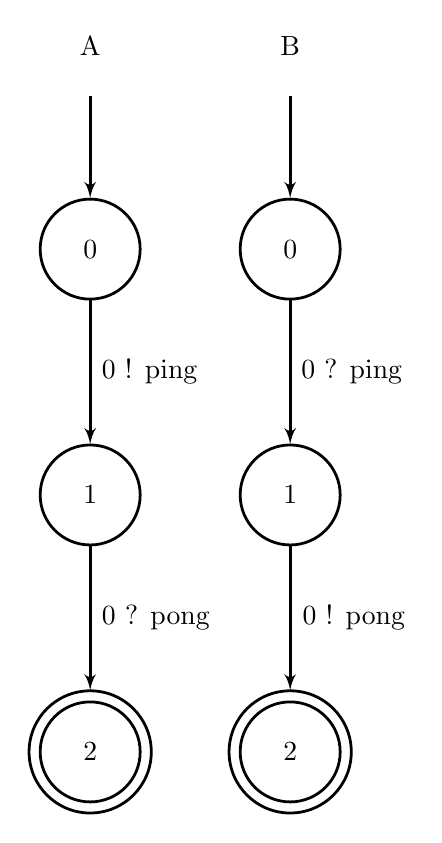
\begin{tikzpicture}[>=latex',line join=bevel,]
  \pgfsetlinewidth{1bp}
%%
\pgfsetcolor{black}
  % Edge: Bdummy -> B0
  \draw [->] (99.0bp,258.17bp) .. controls (99.0bp,250.56bp) and (99.0bp,241.35bp)  .. (99.0bp,221.45bp);
  % Edge: B0 -> B1
  \draw [->] (99.0bp,184.91bp) .. controls (99.0bp,173.26bp) and (99.0bp,157.55bp)  .. (99.0bp,132.85bp);
  \definecolor{strokecol}{rgb}{0.0,0.0,0.0};
  \pgfsetstrokecolor{strokecol}
  \draw (121.12bp,158.75bp) node {0 ? ping};
  % Edge: A1 -> A2
  \draw [->] (27.0bp,96.051bp) .. controls (27.0bp,84.609bp) and (27.0bp,69.297bp)  .. (27.0bp,44.218bp);
  \draw (50.625bp,70.25bp) node {0 ? pong};
  % Edge: A0 -> A1
  \draw [->] (27.0bp,184.91bp) .. controls (27.0bp,173.26bp) and (27.0bp,157.55bp)  .. (27.0bp,132.85bp);
  \draw (48.375bp,158.75bp) node {0 ! ping};
  % Edge: B1 -> B2
  \draw [->] (99.0bp,96.051bp) .. controls (99.0bp,84.609bp) and (99.0bp,69.297bp)  .. (99.0bp,44.218bp);
  \draw (121.88bp,70.25bp) node {0 ! pong};
  % Edge: Adummy -> A0
  \draw [->] (27.0bp,258.17bp) .. controls (27.0bp,250.56bp) and (27.0bp,241.35bp)  .. (27.0bp,221.45bp);
  % Node: A2
\begin{scope}
  \definecolor{strokecol}{rgb}{0.0,0.0,0.0};
  \pgfsetstrokecolor{strokecol}
  \draw (27.0bp,22.0bp) ellipse (18.0bp and 18.0bp);
  \draw (27.0bp,22.0bp) ellipse (22.0bp and 22.0bp);
  \draw (27.0bp,22.0bp) node {2};
\end{scope}
  % Node: Bdummy
\begin{scope}
  \definecolor{strokecol}{rgb}{0.0,0.0,0.0};
  \pgfsetstrokecolor{strokecol}
  % \draw (99.0bp,276.0bp) ellipse (27.0bp and 18.0bp);
  \draw (99.0bp,276.0bp) node {B};
\end{scope}
  % Node: B0
\begin{scope}
  \definecolor{strokecol}{rgb}{0.0,0.0,0.0};
  \pgfsetstrokecolor{strokecol}
  \draw (99.0bp,203.0bp) ellipse (18.0bp and 18.0bp);
  \draw (99.0bp,203.0bp) node {0};
\end{scope}
  % Node: B1
\begin{scope}
  \definecolor{strokecol}{rgb}{0.0,0.0,0.0};
  \pgfsetstrokecolor{strokecol}
  \draw (99.0bp,114.5bp) ellipse (18.0bp and 18.0bp);
  \draw (99.0bp,114.5bp) node {1};
\end{scope}
  % Node: A1
\begin{scope}
  \definecolor{strokecol}{rgb}{0.0,0.0,0.0};
  \pgfsetstrokecolor{strokecol}
  \draw (27.0bp,114.5bp) ellipse (18.0bp and 18.0bp);
  \draw (27.0bp,114.5bp) node {1};
\end{scope}
  % Node: B2
\begin{scope}
  \definecolor{strokecol}{rgb}{0.0,0.0,0.0};
  \pgfsetstrokecolor{strokecol}
  \draw (99.0bp,22.0bp) ellipse (18.0bp and 18.0bp);
  \draw (99.0bp,22.0bp) ellipse (22.0bp and 22.0bp);
  \draw (99.0bp,22.0bp) node {2};
\end{scope}
  % Node: A0
\begin{scope}
  \definecolor{strokecol}{rgb}{0.0,0.0,0.0};
  \pgfsetstrokecolor{strokecol}
  \draw (27.0bp,203.0bp) ellipse (18.0bp and 18.0bp);
  \draw (27.0bp,203.0bp) node {0};
\end{scope}
  % Node: Adummy
\begin{scope}
  \definecolor{strokecol}{rgb}{0.0,0.0,0.0};
  \pgfsetstrokecolor{strokecol}
  % \draw (27.0bp,276.0bp) ellipse (27.0bp and 18.0bp);
  \draw (27.0bp,276.0bp) node {A};
\end{scope}
%
\end{tikzpicture}
\caption{Simple Ping-Pong example.}
\label{fig:ping}
\end{figure}

\end{example}

\section{Progress and Deadlock-Freedom}
I extended \textsc{ReSCu} with verification routines that focus on two
fundamental correctness properties of distributed systems: \emph{progress} and
\emph{deadlock-freedom}. To enable this, the tool constructs the synchronous
system using the synchronous product operation whenever the input SCM is recognized 
as realisable in synchronous communication semantic (RSC). 
Once the system is proven to be RSC, we can safely construct a 
well-formed synchronous product from it, and, given the synchronous product, 
the tool elaborates the other two additional checks.

\textbf{Remark.} 
The discussion in this chapter assumes \emph{complete nondeterministic 
fairness} over choices. In other words, whenever the system encounters 
a nondeterministic branching, all possible continuations are treated 
equally and none of them can be ignored. This assumption ensures that the 
verification does not overlook executions simply because they are less 
probable, and it avoids trivial counterexamples where a branch is never 
explored. In practice, relaxing fairness assumptions can yield more 
realistic analyses (e.g.\ prioritising certain branches or modelling 
schedulers with biases), but at the cost of complicating the 
verification procedures. Exploring weaker or alternative fairness models 
is therefore an interesting direction for future work, especially for 
applications where nondeterminism is influenced by external constraints 
such as message delays or resource contention.

% We consider the definitions given in Chapter~\ref{sec:pre}.
% Definition~\ref{def:cfsm} corresponds to the concept of an SCM.
We now present the
definition of the Synchronous Product for CFSMs, which I have implemented in the
tool, and it serves as a key component for the analysis.

\bigskip

\begin{definition}[Synchronous Product]\label{def:syncprod}
Let $\mathcal{S} = (\mathcal{A}_p)_{p \in \mathbb{P}}$ be a system of CFSMs, where 
$\mathcal{A}_p = (L_p, \mathit{Act}_p, \delta_p, l_{0,p}, F_p)$ is the CFSM associated 
to process $p$.  

The \emph{synchronous product} of $\mathcal{S}$ is the global type 
$P = \mathrm{prod}_s(\mathcal{S}) = (L, \mathit{Arr}, \delta, l_0, F)$,
where
\begin{itemize}
    \item $L = \prod_{p \in \mathbb{P}} L_p$ is the set of global locations,
    \item $l_0 = (l_{0,p})_{p \in \mathbb{P}}$ is the initial global state,
    \item $F = \prod_{p \in \mathbb{P}} F_p$ is the set of global final states,
    \item $\delta$ is the transition relation defined as follows:  
    $(\vec{l}, \; p \xrightarrow{m} q, \; \vec{l}\,') \in \delta$ if
    \[
    (l_p,\, !m^{p \to q},\, l'_p) \in \delta_p, \quad 
    (l_q,\, ?m^{p \to q},\, l'_q) \in \delta_q, \quad 
    l'_r = l_r \;\; \text{for all } r \notin \{p,q\}.
    \]
\end{itemize}
\end{definition}

\bigskip

\begin{example}[Synchronous Product Example]\label{exm:syncping}
Consider the system of CFSMs $\cfsms = (\acfsm_A, \acfsm_B)$ 
from the Example~\ref{exm:ping}. Its synchronous product is 
$P = \mathrm{prod}_s(\cfsms) = (L, \mathit{Arr}, \delta, l_0, F)$,
where
\begin{itemize}
  \item $L = Q_A \times Q_B = \{0,1,2\} \times \{0,1,2\}$,
  \item $l_0 = (0,0)$,
  \item $F = \{(2,2)\}$,
  \item $\delta$ consists of the following transitions:
  $(0,0) \;\xrightarrow{A \xrightarrow{\texttt{ping}} B}\; (1,1)
  \;\xrightarrow{B \xrightarrow{\texttt{pong}} A}\; (2,2)$.
\end{itemize}
Thus, the synchronous product captures the joint behaviour: process $A$ 
sends $\texttt{ping}$ to $B$, then $B$ responds with $\texttt{pong}$ 
to $A$, and both processes reach their final states simultaneously.
Figure~\ref{fig:syncping} illustrates the product's automaton 
$\mathrm{prod}_s(\cfsms)$.

\begin{figure}[!ht]
  \centering
  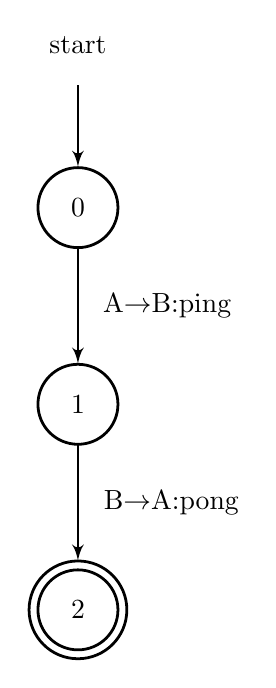
\begin{tikzpicture}[>=latex',line join=bevel,scale=0.8]
    \pgfsetlinewidth{1bp}
  %%
  \pgfsetcolor{black}
    % Edge: A1B1 -> A2B2
    \draw [->] (27.0bp,96.051bp) .. controls (27.0bp,84.609bp) and (27.0bp,69.297bp)  .. (27.0bp,44.218bp);
    \definecolor{strokecol}{rgb}{0.0,0.0,0.0};
    \pgfsetstrokecolor{strokecol}
    \draw (69.0bp,70.25bp) node {B$\to$A:pong};
    % Edge: A0B0 -> A1B1
    \draw [->] (27.0bp,184.91bp) .. controls (27.0bp,173.26bp) and (27.0bp,157.55bp)  .. (27.0bp,132.85bp);
    \draw (67.125bp,158.75bp) node {A$\to$B:ping};
    % Edge: start_node -> A0B0
    \draw [->] (27.0bp,258.17bp) .. controls (27.0bp,250.56bp) and (27.0bp,241.35bp)  .. (27.0bp,221.45bp);
    % Node: A2B2
  \begin{scope}
    \definecolor{strokecol}{rgb}{0.0,0.0,0.0};
    \pgfsetstrokecolor{strokecol}
    \draw (27.0bp,22.0bp) ellipse (18.0bp and 18.0bp);
    \draw (27.0bp,22.0bp) ellipse (22.0bp and 22.0bp);
    \draw (27.0bp,22.0bp) node {2};
  \end{scope}
    % Node: A1B1
  \begin{scope}
    \definecolor{strokecol}{rgb}{0.0,0.0,0.0};
    \pgfsetstrokecolor{strokecol}
    \draw (27.0bp,114.5bp) ellipse (18.0bp and 18.0bp);
    \draw (27.0bp,114.5bp) node {1};
  \end{scope}
    % Node: A0B0
  \begin{scope}
    \definecolor{strokecol}{rgb}{0.0,0.0,0.0};
    \pgfsetstrokecolor{strokecol}
    \draw (27.0bp,203.0bp) ellipse (18.0bp and 18.0bp);
    \draw (27.0bp,203.0bp) node {0};
  \end{scope}
    % Node: start_node
  \begin{scope}
    \definecolor{strokecol}{rgb}{0.0,0.0,0.0};
    \pgfsetstrokecolor{strokecol}
    \draw (27.0bp,276.0bp) node {start};
  \end{scope}
  %
  \end{tikzpicture}
  \caption{Synchronous Product of the CFSM system in Example~\ref{exm:syncping}.}
  \label{fig:syncping}
\end{figure}
% TODO: mostrare pseudo codice dell'algoritmo?
  
\end{example}

After constructing the synchronous product, the tool performs several
important post-processing operations. In particular, it removes any
unreachable nodes from the resulting product, simplifying the structure
and ensuring that only relevant states are retained for further analysis.
We can now define the two SCM properties implemented as verification 
routines in the tool.

Let's consider the defintion of deadlock-freedom for CFSMs 
(Definition~\ref{def:deadlock-free}). I will instanciate the semantic of 
the system, which is $\synchmodel$. This implies 
that the system uses the synchronous product when analysing the 
executions of the system (Definition~\ref{def:syncprod}).

\bigskip

\begin{definition}[Deadlock-freedom in $\synchmodel$]
A system $\cfsms$ is \emph{deadlock-free} in $\synchmodel$  
if for every execution 
$e \in \executionsofcfsms{\acceptcompletion{\cfsms}}{\synchmodel}$,  
there exists a completion $e'$ with $e \prefixorder e'$ and  
$e' \in \executionsofcfsms{\cfsms}{\synchmodel}$.  
\end{definition}

\textbf{Remark.} The notation $\acceptcompletion{\cfsms}$ denotes the 
system obtained by treating every state as an accepting (or final) state. 
In this way, all possible partial executions of the system are taken 
into account. The deadlock-freedom condition then requires that each 
such partial execution can be extended to a complete execution of the 
original system $\cfsms$. Intuitively, this ensures that the system 
cannot ``get stuck'' in the middle of a computation, i.e.\ every 
execution fragment can always be continued.  

More precisely, a system that can reach, from its initial states, some state
that does not lead to a final state is not deadlock-free. Under this definition,
even a loop that never reaches a final state is considered a deadlock,
making the property more restrictive. This check is implemented using a
reverse search algorithm starting from the final states.

% TODO: mostrare pseudo codice dell'algoritmo?

% TODO: Specificare che questa nozione di deadlock-freedom vale per il paper di cinzia
% Vale ancora questo todo?

\bigskip

\begin{definition}[Progress]\label{def:progress}
A system of CFSMs $\cfsms$ satisfies the \emph{progress} property in $\rscmodel$
if for every execution $e \in \executionsofcfsms{\acceptcompletion{P}}{}$, 
with $P = \mathrm{prod}_s(\cfsms)$,
\begin{itemize}
    \item the execution $e$ is also a valid execution of $e\in \executionsofcfsms{P}{}$, or
    \item there exists another execution $e'\in\executionsofcfsms{\acceptcompletion{P}}{}$
          such that $e \prefixorder e'$, with $e \neq e'$.
\end{itemize}
\end{definition}

Intuitively, progress ensures that the system never reaches a state
where it is permanently stuck, except in the case of successful termination.
This is weaker than deadlock-freedom, since infinite executions are allowed
as long as they can always perform a new step. In particular, livelocks
(loops without termination) are considered to satisfy progress, but would
violate deadlock-freedom.

% TODO: mostrare pseudo codice dell'algoritmo?

% \section{Verification Algorithms}

% The verification of \emph{deadlock-freedom} and \emph{progress}
% properties in \textsc{ReSCu} are based on a classical
% \emph{reverse search} algorithm~\cite{avis1996reverse}.
% The idea is to initialise the search from ``bad'' states
% (deadlock or non-progress states) and traverse the system graph
% backwards, collecting all states that can eventually reach one of these
% bad states. If the initial state is discovered during the traversal,
% the property does not hold. Otherwise, the property is satisfied.  

% This approach is widely used in model checking since it reduces the
% problem to a systematic graph exploration, avoiding redundant
% re-computation~\cite{padovani2014deadlock}. The two algorithms below
% are specialisations of this method.

% \begin{algorithm}[H]
% \caption{Deadlock Freedom via Reverse Search}
% \label{alg:reverse-search-deadlock}
% \KwIn{System $\mathcal{S}$, initial state $s_0$}
% \KwOut{True if $\mathcal{S}$ is deadlock-free, False otherwise}

% $Visited \gets \emptyset$\;
% $Worklist \gets \{ \text{deadlock states of } \mathcal{S} \}$\;

% \While{$Worklist \neq \emptyset$}{
%     remove $s$ from $Worklist$\;
%     \If{$s \notin Visited$}{
%         add $s$ to $Visited$\;
%         \ForEach{predecessor $p$ of $s$ in $\mathcal{S}$}{
%             add $p$ to $Worklist$\;
%         }
%     }
% }

% \If{$s_0 \in Visited$}{
%     \Return False \tcp*{deadlock is reachable}
% }
% \Return True \tcp*{system is deadlock-free}
% \end{algorithm}

% \begin{algorithm}[H]
% \caption{Progress via Reverse Search}
% \label{alg:reverse-search-progress}
% \KwIn{System $\mathcal{S}$, initial state $s_0$}
% \KwOut{True if $\mathcal{S}$ ensures progress, False otherwise}

% $Visited \gets \emptyset$\;
% $Worklist \gets \{ \text{non-final states with no outgoing transitions} \}$\;

% \While{$Worklist \neq \emptyset$}{
%     remove $s$ from $Worklist$\;
%     \If{$s \notin Visited$}{
%         add $s$ to $Visited$\;
%         \ForEach{predecessor $p$ of $s$ in $\mathcal{S}$}{
%             add $p$ to $Worklist$\;
%         }
%     }
% }

% \If{$s_0 \in Visited$}{
%     \Return False \tcp*{initial state can lead to non-progress}
% }
% \Return True \tcp*{system guarantees progress}
% \end{algorithm}

Lastly, the synchronized system can be exported in DOT format
(with a default filename of \verb|sync.dot|), which allows for graphical 
visualization of its structure and behaviour. Some illustrative examples 
demonstrating these new features are included in the
\verb|examples/deadlock| folder from the online repository~\cite{rescurepo}.
Two of them are showed and explained with details in the next section.

% TODO: CINZIA, X TESI:
% pensare ad un esempio che fa vedere che non è vero in generale

\section{Examples}

To illustrate these notions, I present two examples. The first is the
classical \emph{Dining Philosophers} problem, which shows how resource
contention can lead to deadlock. The second is a minimal looping system
that demonstrates how a process may satisfy the progress property while
still failing to be deadlock-free.

\subsection{The Dining Philosophers}

% TODO: mettere anche versione giusta?
\begin{example}\label{exm:philo}
Consider two philosophers $P_0, P_1$ and two forks $F_1, F_2$, arranged
so that each philosopher needs both forks to eat. If both philosophers
pick up their left fork simultaneously, each waits indefinitely for the
other fork, producing a deadlock. This captures the essence of the Dining
Philosophers problem: concurrent processes blocking one another when
competing for shared resources.

\bigskip

\begin{lstlisting}[language={},caption={Output of Example~\ref{exm:philo}},
    label={lst:philo}]
This system is RSC.
There are some sink states:
Sink: Id=11 Configuration={{ F0:4; F1:3; P1:2; P2:2 }}
There are some deadlock states:
Deadlock: Id=4 Configuration={{ F0:2; F1:1; P1:1; P2:1 }}
Deadlock: Id=11 Configuration={{ F0:4; F1:3; P1:2; P2:2 }}
Deadlock: Id=8 Configuration={{ F0:4; F1:1; P1:1; P2:2 }}
Deadlock: Id=7 Configuration={{ F0:2; F1:3; P1:2; P2:1 }}
\end{lstlisting}

The behaviour of the four participants is shown in
Figure~\ref{fig:philo}. Running the tool on
this input produces the terminal output in
Listing~\ref{lst:philo} and the corresponding synchronous system in
Figure~\ref{fig:philo-sync}. In the
generated figure, the red state marks a configuration where no further
actions are possible, while the three yellow states correspond to
deadlocks, i.e.\ executions where both philosophers wait for each other
indefinitely. The terminal output also lists the precise configurations
of these problematic states.

\newpage

\begin{figure}[!ht]
    \centering
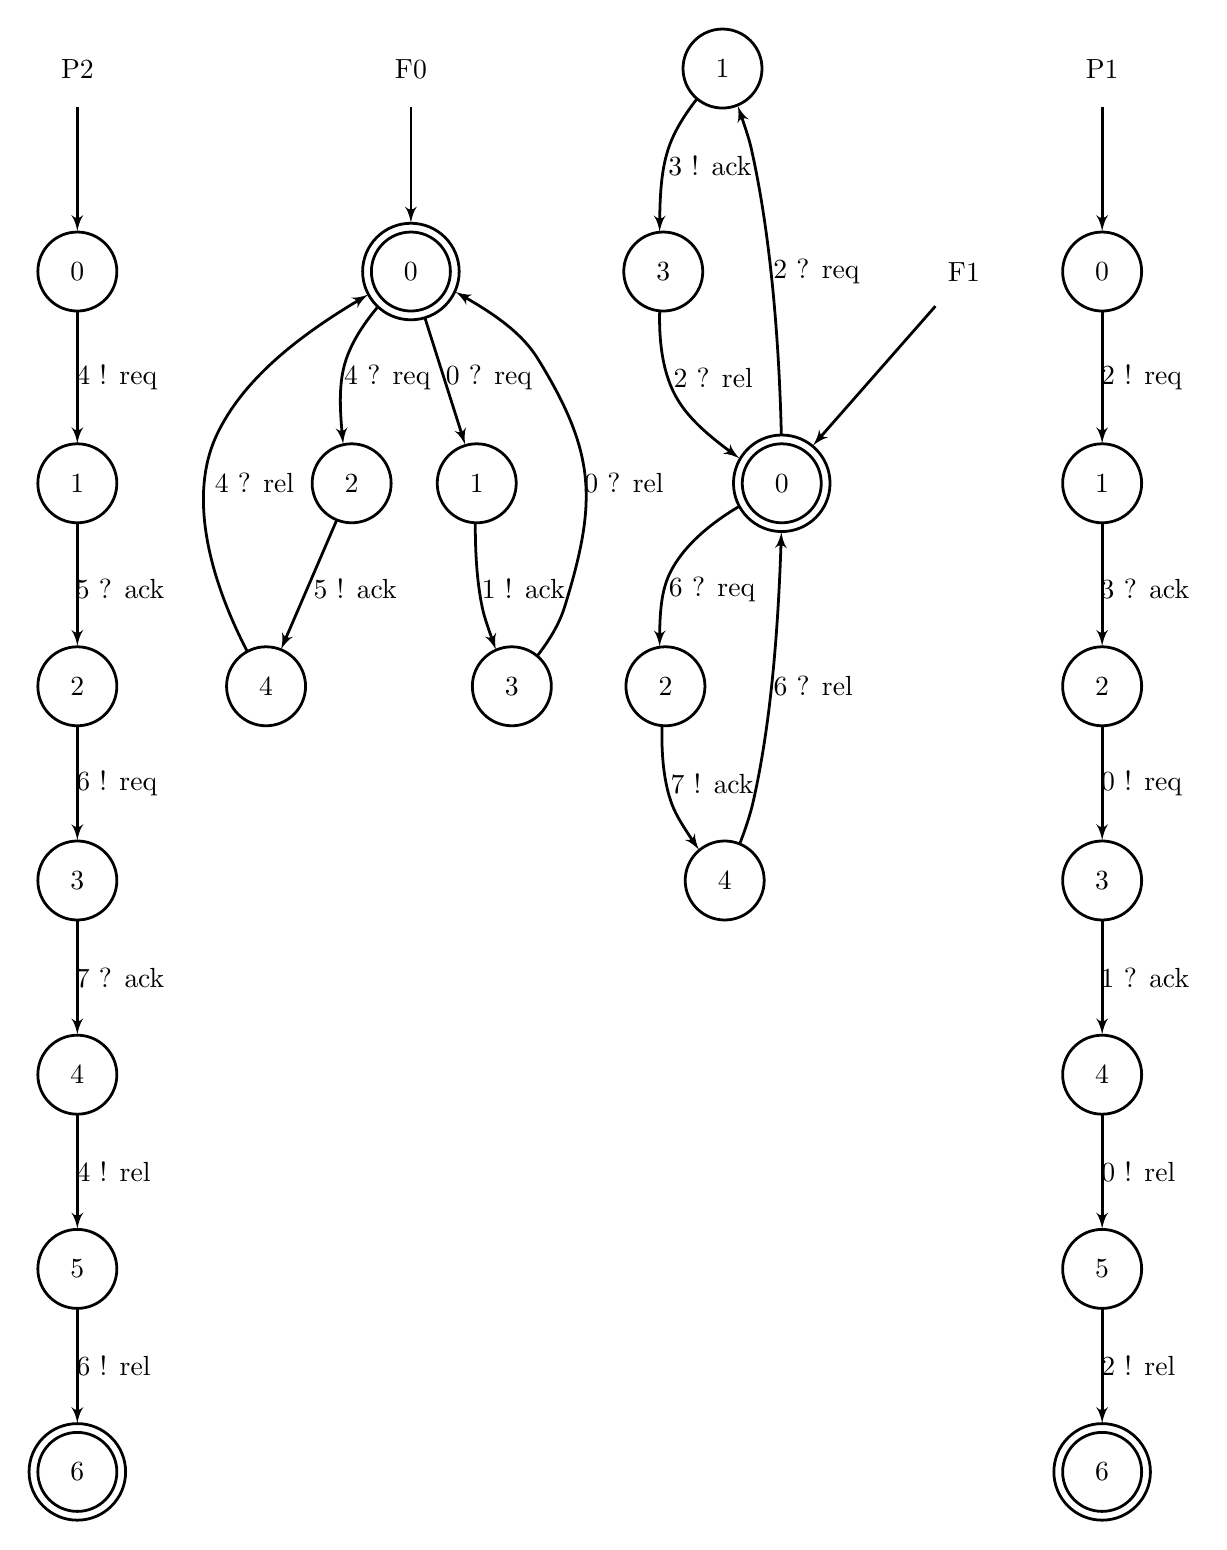
\begin{tikzpicture}[>=latex',line join=bevel,scale=0.79]
  \pgfsetlinewidth{1bp}
%%
\pgfsetcolor{black}
  % Edge: P23 -> P24
  \draw [->] (27.0bp,273.41bp) .. controls (27.0bp,261.76bp) and (27.0bp,246.05bp)  .. (27.0bp,221.35bp);
  \definecolor{strokecol}{rgb}{0.0,0.0,0.0};
  \pgfsetstrokecolor{strokecol}
  \draw (46.5bp,247.25bp) node {7 ? ack};
  % Edge: F00 -> F02
  \draw [->] (163.75bp,552.68bp) .. controls (158.12bp,545.99bp) and (152.42bp,537.69bp)  .. (149.5bp,529.0bp) .. controls (146.63bp,520.45bp) and (146.19bp,510.74bp)  .. (148.12bp,490.45bp);
  \draw (168.25bp,520.75bp) node {4 ? req};
  % Edge: F00 -> F01
  \draw [->] (185.51bp,547.49bp) .. controls (189.85bp,533.83bp) and (195.6bp,515.7bp)  .. (203.7bp,490.19bp);
  \draw (214.55bp,520.75bp) node {0 ? req};
  % Edge: F11 -> F13
  \draw [->] (309.26bp,647.53bp) .. controls (304.38bp,641.32bp) and (299.22bp,633.51bp)  .. (296.5bp,625.5bp) .. controls (293.62bp,617.02bp) and (292.5bp,607.4bp)  .. (292.34bp,587.21bp);
  \draw (315.25bp,617.25bp) node {3 ! ack};
  % Edge: F02 -> F04
  \draw [->] (145.21bp,455.74bp) .. controls (139.43bp,442.32bp) and (131.01bp,422.79bp)  .. (119.85bp,396.89bp);
  \draw (153.59bp,424.25bp) node {5 ! ack};
  % Edge: P21 -> P22
  \draw [->] (27.0bp,454.05bp) .. controls (27.0bp,441.53bp) and (27.0bp,424.37bp)  .. (27.0bp,398.4bp);
  \draw (46.5bp,424.25bp) node {5 ? ack};
  % Edge: P1dummy -> P10
  \draw [->] (494.0bp,643.9bp) .. controls (494.0bp,631.26bp) and (494.0bp,613.55bp)  .. (494.0bp,587.42bp);
  % Edge: F10 -> F11
  \draw [->] (347.8bp,494.92bp) .. controls (347.12bp,524.61bp) and (344.41bp,579.76bp)  .. (334.0bp,625.5bp) .. controls (333.39bp,628.17bp) and (332.63bp,630.9bp)  .. (328.0bp,644.39bp);
  \draw (363.84bp,569.0bp) node {2 ? req};
  % Edge: F10 -> F12
  \draw [->] (328.44bp,461.89bp) .. controls (317.28bp,455.28bp) and (304.21bp,445.37bp)  .. (297.5bp,432.5bp) .. controls (293.87bp,425.54bp) and (292.43bp,417.31bp)  .. (292.34bp,398.17bp);
  \draw (316.25bp,424.25bp) node {6 ? req};
  % Edge: P15 -> P16
  \draw [->] (494.0bp,96.051bp) .. controls (494.0bp,84.609bp) and (494.0bp,69.297bp)  .. (494.0bp,44.218bp);
  \draw (510.5bp,70.25bp) node {2 ! rel};
  % Edge: F14 -> F10
  \draw [->] (329.0bp,308.61bp) .. controls (331.27bp,314.45bp) and (333.57bp,321.18bp)  .. (335.0bp,327.5bp) .. controls (343.53bp,365.15bp) and (346.5bp,409.54bp)  .. (347.83bp,450.24bp);
  \draw (362.3bp,380.0bp) node {6 ? rel};
  % Edge: P11 -> P12
  \draw [->] (494.0bp,454.05bp) .. controls (494.0bp,441.53bp) and (494.0bp,424.37bp)  .. (494.0bp,398.4bp);
  \draw (513.5bp,424.25bp) node {3 ? ack};
  % Edge: P10 -> P11
  \draw [->] (494.0bp,550.67bp) .. controls (494.0bp,537.08bp) and (494.0bp,517.89bp)  .. (494.0bp,490.72bp);
  \draw (512.0bp,520.75bp) node {2 ! req};
  % Edge: P12 -> P13
  \draw [->] (494.0bp,361.91bp) .. controls (494.0bp,350.26bp) and (494.0bp,334.55bp)  .. (494.0bp,309.85bp);
  \draw (512.0bp,335.75bp) node {0 ! req};
  % Edge: F12 -> F14
  \draw [->] (293.48bp,361.86bp) .. controls (293.15bp,351.62bp) and (293.73bp,338.51bp)  .. (297.5bp,327.5bp) .. controls (299.0bp,323.12bp) and (301.22bp,318.8bp)  .. (310.27bp,305.48bp);
  \draw (316.25bp,335.75bp) node {7 ! ack};
  % Edge: F1dummy -> F10
  \draw [->] (418.03bp,553.23bp) .. controls (405.14bp,538.56bp) and (385.13bp,515.78bp)  .. (362.27bp,489.75bp);
  % Edge: P13 -> P14
  \draw [->] (494.0bp,273.41bp) .. controls (494.0bp,261.76bp) and (494.0bp,246.05bp)  .. (494.0bp,221.35bp);
  \draw (513.5bp,247.25bp) node {1 ? ack};
  % Edge: F04 -> F00
  \draw [->] (104.36bp,396.04bp) .. controls (92.695bp,418.48bp) and (75.05bp,461.59bp)  .. (90.5bp,494.5bp) .. controls (102.62bp,520.33bp) and (128.78bp,540.22bp)  .. (159.49bp,558.47bp);
  \draw (107.75bp,472.5bp) node {4 ? rel};
  % Edge: P24 -> P25
  \draw [->] (27.0bp,184.91bp) .. controls (27.0bp,173.26bp) and (27.0bp,157.55bp)  .. (27.0bp,132.85bp);
  \draw (43.5bp,158.75bp) node {4 ! rel};
  % Edge: F01 -> F03
  \draw [->] (208.36bp,454.32bp) .. controls (208.29bp,443.26bp) and (208.85bp,428.65bp)  .. (211.5bp,416.0bp) .. controls (212.1bp,413.16bp) and (212.89bp,410.24bp)  .. (217.7bp,396.7bp);
  \draw (230.25bp,424.25bp) node {1 ! ack};
  % Edge: F03 -> F00
  \draw [->] (236.67bp,393.95bp) .. controls (241.48bp,400.16bp) and (246.51bp,407.98bp)  .. (249.0bp,416.0bp) .. controls (263.95bp,464.24bp) and (263.45bp,485.98bp)  .. (237.0bp,529.0bp) .. controls (230.4bp,539.73bp) and (219.62bp,548.17bp)  .. (199.3bp,559.73bp);
  \draw (276.13bp,472.5bp) node {0 ? rel};
  % Edge: P14 -> P15
  \draw [->] (494.0bp,184.91bp) .. controls (494.0bp,173.26bp) and (494.0bp,157.55bp)  .. (494.0bp,132.85bp);
  \draw (510.5bp,158.75bp) node {0 ! rel};
  % Edge: P2dummy -> P20
  \draw [->] (27.0bp,643.9bp) .. controls (27.0bp,631.26bp) and (27.0bp,613.55bp)  .. (27.0bp,587.42bp);
  % Edge: P25 -> P26
  \draw [->] (27.0bp,96.051bp) .. controls (27.0bp,84.609bp) and (27.0bp,69.297bp)  .. (27.0bp,44.218bp);
  \draw (43.5bp,70.25bp) node {6 ! rel};
  % Edge: P20 -> P21
  \draw [->] (27.0bp,550.67bp) .. controls (27.0bp,537.08bp) and (27.0bp,517.89bp)  .. (27.0bp,490.72bp);
  \draw (45.0bp,520.75bp) node {4 ! req};
  % Edge: F0dummy -> F00
  \draw [->] (179.0bp,643.9bp) .. controls (179.0bp,632.34bp) and (179.0bp,616.54bp)  .. (179.0bp,591.29bp);
  % Edge: F13 -> F10
  \draw [->] (292.37bp,550.99bp) .. controls (292.04bp,539.46bp) and (293.14bp,524.25bp)  .. (299.5bp,512.5bp) .. controls (304.18bp,503.85bp) and (311.66bp,496.43bp)  .. (328.69bp,483.88bp);
  \draw (316.75bp,520.75bp) node {2 ? rel};
  % Edge: P22 -> P23
  \draw [->] (27.0bp,361.91bp) .. controls (27.0bp,350.26bp) and (27.0bp,334.55bp)  .. (27.0bp,309.85bp);
  \draw (45.0bp,335.75bp) node {6 ! req};
  % Node: P23
\begin{scope}
  \definecolor{strokecol}{rgb}{0.0,0.0,0.0};
  \pgfsetstrokecolor{strokecol}
  \draw (27.0bp,291.5bp) ellipse (18.0bp and 18.0bp);
  \draw (27.0bp,291.5bp) node {3};
\end{scope}
  % Node: P24
\begin{scope}
  \definecolor{strokecol}{rgb}{0.0,0.0,0.0};
  \pgfsetstrokecolor{strokecol}
  \draw (27.0bp,203.0bp) ellipse (18.0bp and 18.0bp);
  \draw (27.0bp,203.0bp) node {4};
\end{scope}
  % Node: F00
\begin{scope}
  \definecolor{strokecol}{rgb}{0.0,0.0,0.0};
  \pgfsetstrokecolor{strokecol}
  \draw (179.0bp,569.0bp) ellipse (18.0bp and 18.0bp);
  \draw (179.0bp,569.0bp) ellipse (22.0bp and 22.0bp);
  \draw (179.0bp,569.0bp) node {0};
\end{scope}
  % Node: F02
\begin{scope}
  \definecolor{strokecol}{rgb}{0.0,0.0,0.0};
  \pgfsetstrokecolor{strokecol}
  \draw (152.0bp,472.5bp) ellipse (18.0bp and 18.0bp);
  \draw (152.0bp,472.5bp) node {2};
\end{scope}
  % Node: F01
\begin{scope}
  \definecolor{strokecol}{rgb}{0.0,0.0,0.0};
  \pgfsetstrokecolor{strokecol}
  \draw (209.0bp,472.5bp) ellipse (18.0bp and 18.0bp);
  \draw (209.0bp,472.5bp) node {1};
\end{scope}
  % Node: F11
\begin{scope}
  \definecolor{strokecol}{rgb}{0.0,0.0,0.0};
  \pgfsetstrokecolor{strokecol}
  \draw (321.0bp,661.5bp) ellipse (18.0bp and 18.0bp);
  \draw (321.0bp,661.5bp) node {1};
\end{scope}
  % Node: F13
\begin{scope}
  \definecolor{strokecol}{rgb}{0.0,0.0,0.0};
  \pgfsetstrokecolor{strokecol}
  \draw (294.0bp,569.0bp) ellipse (18.0bp and 18.0bp);
  \draw (294.0bp,569.0bp) node {3};
\end{scope}
  % Node: F04
\begin{scope}
  \definecolor{strokecol}{rgb}{0.0,0.0,0.0};
  \pgfsetstrokecolor{strokecol}
  \draw (113.0bp,380.0bp) ellipse (18.0bp and 18.0bp);
  \draw (113.0bp,380.0bp) node {4};
\end{scope}
  % Node: P21
\begin{scope}
  \definecolor{strokecol}{rgb}{0.0,0.0,0.0};
  \pgfsetstrokecolor{strokecol}
  \draw (27.0bp,472.5bp) ellipse (18.0bp and 18.0bp);
  \draw (27.0bp,472.5bp) node {1};
\end{scope}
  % Node: P22
\begin{scope}
  \definecolor{strokecol}{rgb}{0.0,0.0,0.0};
  \pgfsetstrokecolor{strokecol}
  \draw (27.0bp,380.0bp) ellipse (18.0bp and 18.0bp);
  \draw (27.0bp,380.0bp) node {2};
\end{scope}
  % Node: P1dummy
\begin{scope}
  \definecolor{strokecol}{rgb}{0.0,0.0,0.0};
  \pgfsetstrokecolor{strokecol}
  % \draw (494.0bp,661.5bp) ellipse (27.0bp and 18.0bp);
  \draw (494.0bp,661.5bp) node {P1};
\end{scope}
  % Node: P10
\begin{scope}
  \definecolor{strokecol}{rgb}{0.0,0.0,0.0};
  \pgfsetstrokecolor{strokecol}
  \draw (494.0bp,569.0bp) ellipse (18.0bp and 18.0bp);
  \draw (494.0bp,569.0bp) node {0};
\end{scope}
  % Node: F10
\begin{scope}
  \definecolor{strokecol}{rgb}{0.0,0.0,0.0};
  \pgfsetstrokecolor{strokecol}
  \draw (348.0bp,472.5bp) ellipse (18.0bp and 18.0bp);
  \draw (348.0bp,472.5bp) ellipse (22.0bp and 22.0bp);
  \draw (348.0bp,472.5bp) node {0};
\end{scope}
  % Node: F12
\begin{scope}
  \definecolor{strokecol}{rgb}{0.0,0.0,0.0};
  \pgfsetstrokecolor{strokecol}
  \draw (295.0bp,380.0bp) ellipse (18.0bp and 18.0bp);
  \draw (295.0bp,380.0bp) node {2};
\end{scope}
  % Node: P15
\begin{scope}
  \definecolor{strokecol}{rgb}{0.0,0.0,0.0};
  \pgfsetstrokecolor{strokecol}
  \draw (494.0bp,114.5bp) ellipse (18.0bp and 18.0bp);
  \draw (494.0bp,114.5bp) node {5};
\end{scope}
  % Node: P16
\begin{scope}
  \definecolor{strokecol}{rgb}{0.0,0.0,0.0};
  \pgfsetstrokecolor{strokecol}
  \draw (494.0bp,22.0bp) ellipse (18.0bp and 18.0bp);
  \draw (494.0bp,22.0bp) ellipse (22.0bp and 22.0bp);
  \draw (494.0bp,22.0bp) node {6};
\end{scope}
  % Node: F14
\begin{scope}
  \definecolor{strokecol}{rgb}{0.0,0.0,0.0};
  \pgfsetstrokecolor{strokecol}
  \draw (322.0bp,291.5bp) ellipse (18.0bp and 18.0bp);
  \draw (322.0bp,291.5bp) node {4};
\end{scope}
  % Node: P11
\begin{scope}
  \definecolor{strokecol}{rgb}{0.0,0.0,0.0};
  \pgfsetstrokecolor{strokecol}
  \draw (494.0bp,472.5bp) ellipse (18.0bp and 18.0bp);
  \draw (494.0bp,472.5bp) node {1};
\end{scope}
  % Node: P12
\begin{scope}
  \definecolor{strokecol}{rgb}{0.0,0.0,0.0};
  \pgfsetstrokecolor{strokecol}
  \draw (494.0bp,380.0bp) ellipse (18.0bp and 18.0bp);
  \draw (494.0bp,380.0bp) node {2};
\end{scope}
  % Node: P13
\begin{scope}
  \definecolor{strokecol}{rgb}{0.0,0.0,0.0};
  \pgfsetstrokecolor{strokecol}
  \draw (494.0bp,291.5bp) ellipse (18.0bp and 18.0bp);
  \draw (494.0bp,291.5bp) node {3};
\end{scope}
  % Node: P26
\begin{scope}
  \definecolor{strokecol}{rgb}{0.0,0.0,0.0};
  \pgfsetstrokecolor{strokecol}
  \draw (27.0bp,22.0bp) ellipse (18.0bp and 18.0bp);
  \draw (27.0bp,22.0bp) ellipse (22.0bp and 22.0bp);
  \draw (27.0bp,22.0bp) node {6};
\end{scope}
  % Node: F1dummy
\begin{scope}
  \definecolor{strokecol}{rgb}{0.0,0.0,0.0};
  \pgfsetstrokecolor{strokecol}
  % \draw (431.0bp,569.0bp) ellipse (27.0bp and 18.0bp);
  \draw (431.0bp,569.0bp) node {F1};
\end{scope}
  % Node: P14
\begin{scope}
  \definecolor{strokecol}{rgb}{0.0,0.0,0.0};
  \pgfsetstrokecolor{strokecol}
  \draw (494.0bp,203.0bp) ellipse (18.0bp and 18.0bp);
  \draw (494.0bp,203.0bp) node {4};
\end{scope}
  % Node: P25
\begin{scope}
  \definecolor{strokecol}{rgb}{0.0,0.0,0.0};
  \pgfsetstrokecolor{strokecol}
  \draw (27.0bp,114.5bp) ellipse (18.0bp and 18.0bp);
  \draw (27.0bp,114.5bp) node {5};
\end{scope}
  % Node: F03
\begin{scope}
  \definecolor{strokecol}{rgb}{0.0,0.0,0.0};
  \pgfsetstrokecolor{strokecol}
  \draw (225.0bp,380.0bp) ellipse (18.0bp and 18.0bp);
  \draw (225.0bp,380.0bp) node {3};
\end{scope}
  % Node: P2dummy
\begin{scope}
  \definecolor{strokecol}{rgb}{0.0,0.0,0.0};
  \pgfsetstrokecolor{strokecol}
  % \draw (27.0bp,661.5bp) ellipse (27.0bp and 18.0bp);
  \draw (27.0bp,661.5bp) node {P2};
\end{scope}
  % Node: P20
\begin{scope}
  \definecolor{strokecol}{rgb}{0.0,0.0,0.0};
  \pgfsetstrokecolor{strokecol}
  \draw (27.0bp,569.0bp) ellipse (18.0bp and 18.0bp);
  \draw (27.0bp,569.0bp) node {0};
\end{scope}
  % Node: F0dummy
\begin{scope}
  \definecolor{strokecol}{rgb}{0.0,0.0,0.0};
  \pgfsetstrokecolor{strokecol}
  % \draw (179.0bp,661.5bp) ellipse (27.0bp and 18.0bp);
  \draw (179.0bp,661.5bp) node {F0};
\end{scope}
%
\end{tikzpicture}
    \caption{SCM automata representation of the Example~\ref{exm:philo}.}
    \label{fig:philo}
\end{figure}

\newpage

\begin{figure}[!ht]
    \centering

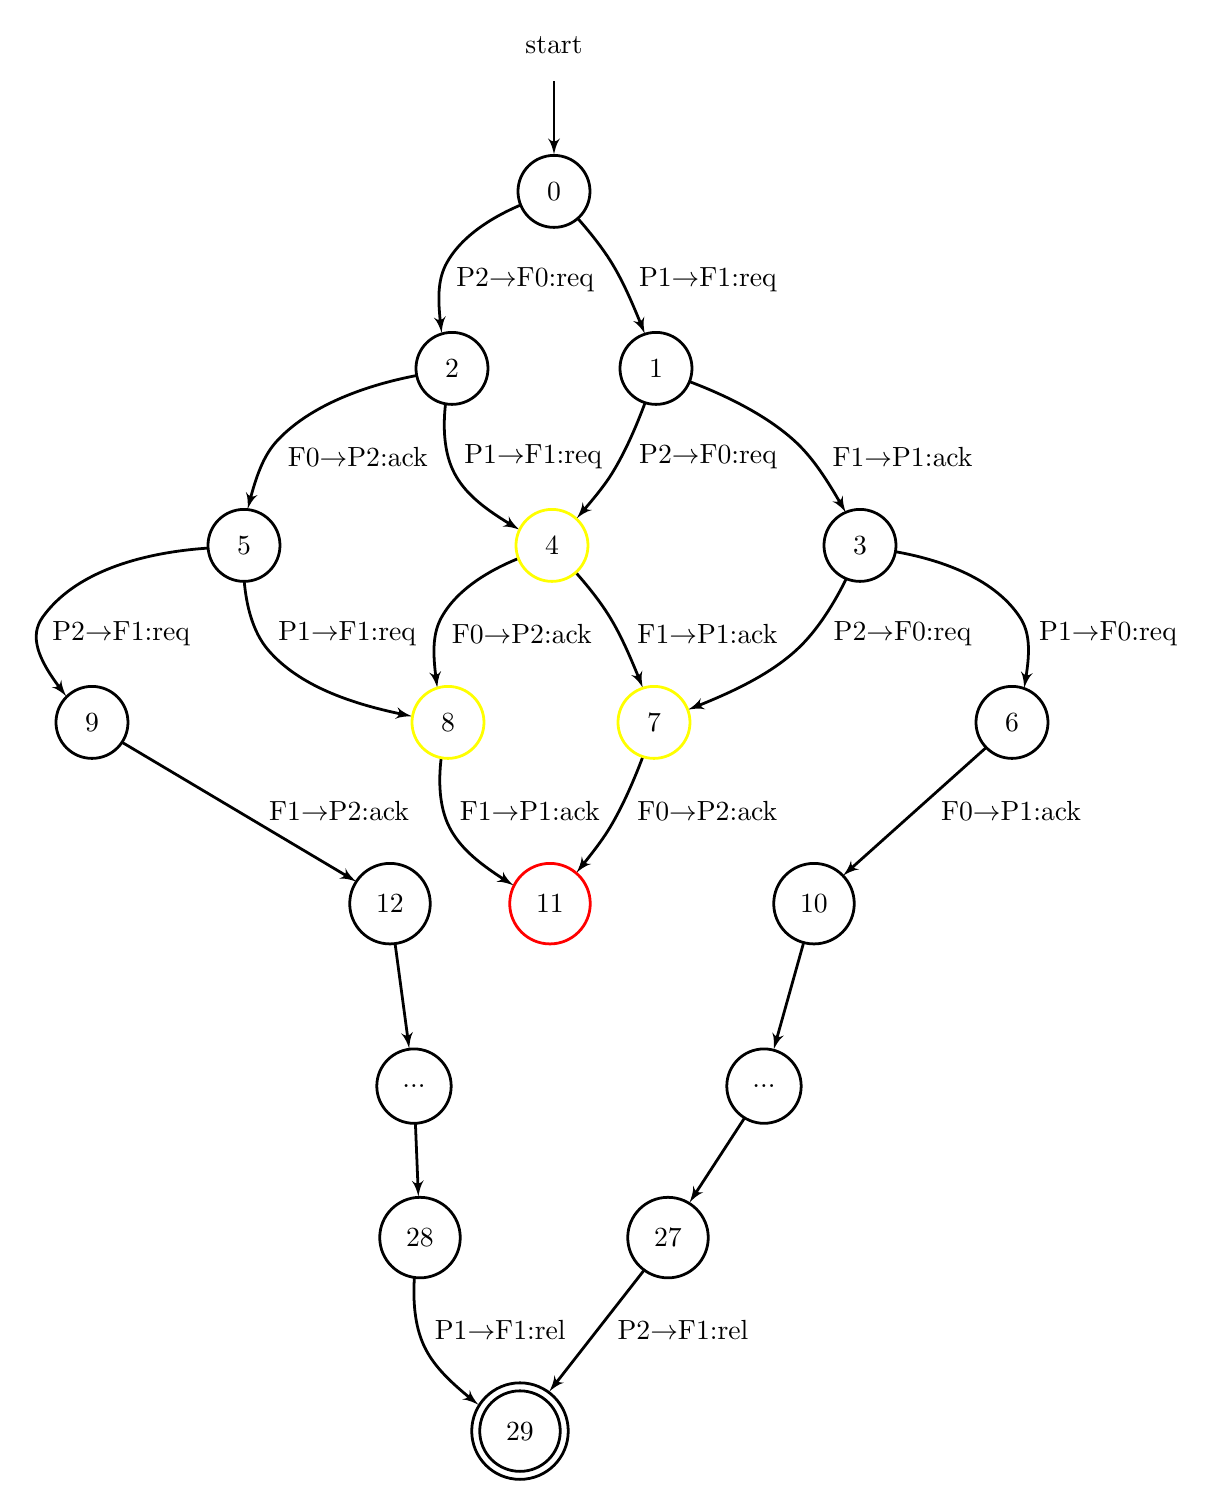
\begin{tikzpicture}[>=latex',line join=bevel,scale=0.72]
  \pgfsetlinewidth{1bp}
%%
\pgfsetcolor{black}
  % Edge: F02F10P10P21 -> F04F10P10P22
  \draw [->] (190.31bp,551.88bp) .. controls (170.67bp,548.11bp) and (139.47bp,539.27bp)  .. (120.97bp,519.48bp) .. controls (114.96bp,513.06bp) and (111.11bp,504.46bp)  .. (106.05bp,485.16bp);
  \definecolor{strokecol}{rgb}{0.0,0.0,0.0};
  \pgfsetstrokecolor{strokecol}
  \draw (161.09bp,511.23bp) node {F0$\to$P2:ack};
  % Edge: F02F10P10P21 -> F02F11P11P21
  \draw [->] (204.93bp,537.28bp) .. controls (203.79bp,526.78bp) and (203.95bp,513.42bp)  .. (209.47bp,502.98bp) .. controls (214.49bp,493.47bp) and (223.38bp,485.95bp)  .. (241.94bp,474.84bp);
  \draw (248.84bp,511.23bp) node {P1$\to$F1:req};
  % Edge: F00F11P11P20 -> F00F13P12P20
  \draw [->] (327.34bp,548.73bp) .. controls (342.31bp,543.07bp) and (363.97bp,533.26bp)  .. (379.22bp,519.48bp) .. controls (387.26bp,512.21bp) and (394.13bp,502.55bp)  .. (405.07bp,483.5bp);
  \draw (433.49bp,511.23bp) node {F1$\to$P1:ack};
  % Edge: F00F11P11P20 -> F02F11P11P21
  \draw [->] (304.68bp,538.08bp) .. controls (300.8bp,527.63bp) and (295.1bp,514.04bp)  .. (288.22bp,502.98bp) .. controls (285.26bp,498.22bp) and (281.67bp,493.44bp)  .. (270.63bp,480.53bp);
  \draw (336.25bp,511.23bp) node {P2$\to$F0:req};
  % Edge: F00F14P16P25 -> F00F10P16P26
  \draw [->] (304.33bp,104.67bp) .. controls (293.44bp,90.719bp) and (277.04bp,69.729bp)  .. (256.88bp,43.906bp);
  \draw (323.72bp,74.512bp) node {P2$\to$F1:rel};
  % Edge: F00F10P10P20 -> F02F10P10P21
  \draw [->] (242.27bp,637.06bp) .. controls (229.61bp,631.64bp) and (213.22bp,622.27bp)  .. (205.47bp,607.98bp) .. controls (201.63bp,600.89bp) and (200.83bp,592.42bp)  .. (203.04bp,573.23bp);
  \draw (244.84bp,599.73bp) node {P2$\to$F0:req};
  % Edge: F00F10P10P20 -> F00F11P11P20
  \draw [->] (271.19bp,630.36bp) .. controls (276.83bp,623.98bp) and (283.37bp,615.93bp)  .. (288.22bp,607.98bp) .. controls (292.88bp,600.33bp) and (297.04bp,591.52bp)  .. (304.61bp,572.84bp);
  \draw (336.18bp,599.73bp) node {P1$\to$F1:req};
  % Edge: F04F10P10P22 -> F04F11P11P22
  \draw [->] (104.36bp,448.85bp) .. controls (105.32bp,437.85bp) and (108.26bp,423.91bp)  .. (116.47bp,414.48bp) .. controls (131.82bp,396.84bp) and (157.16bp,388.03bp)  .. (188.23bp,381.53bp);
  \draw (155.84bp,422.73bp) node {P1$\to$F1:req};
  % Edge: F04F10P10P22 -> F04F12P10P23
  \draw [->] (85.982bp,465.61bp) .. controls (62.433bp,464.04bp) and (22.249bp,457.38bp)  .. (3.468bp,430.98bp) .. controls (-3.2418bp,421.54bp) and (1.3095bp,410.01bp)  .. (15.345bp,391.56bp);
  \draw (42.843bp,422.73bp) node {P2$\to$F1:req};
  % Edge: F04F14P10P24 -> F00F14P10P25
  \draw [->] (179.82bp,267.49bp) .. controls (181.43bp,255.51bp) and (183.53bp,239.92bp)  .. (186.82bp,215.43bp);
  % \draw (222.17bp,241.47bp) node {P2$\to$F0:rel};
  % Edge: F00F13P15P26 -> F00F10P16P26
  \draw [->] (189.41bp,100.63bp) .. controls (188.73bp,89.988bp) and (189.35bp,76.831bp)  .. (194.47bp,66.262bp) .. controls (198.56bp,57.814bp) and (205.27bp,50.41bp)  .. (221.45bp,37.266bp);
  \draw (232.34bp,74.512bp) node {P1$\to$F1:rel};
  % Edge: F00F13P12P20 -> F01F13P13P20
  \draw [->] (430.17bp,463.79bp) .. controls (449.25bp,460.4bp) and (478.53bp,451.91bp)  .. (492.22bp,430.98bp) .. controls (496.82bp,423.94bp) and (497.52bp,415.14bp)  .. (494.3bp,395.62bp);
  \draw (536.24bp,422.73bp) node {P1$\to$F0:req};
  % Edge: F00F13P12P20 -> F02F13P12P21
  \draw [->] (405.19bp,449.94bp) .. controls (399.68bp,438.85bp) and (391.14bp,424.38bp)  .. (380.22bp,414.48bp) .. controls (367.77bp,403.19bp) and (351.01bp,394.7bp)  .. (326.28bp,384.84bp);
  \draw (433.49bp,422.73bp) node {P2$\to$F0:req};
  % Edge: F02F11P11P21 -> F04F11P11P22
  \draw [->] (241.08bp,460.3bp) .. controls (228.04bp,454.97bp) and (211.02bp,445.6bp)  .. (202.97bp,430.98bp) .. controls (199.02bp,423.81bp) and (198.31bp,415.19bp)  .. (200.87bp,395.78bp);
  \draw (243.09bp,422.73bp) node {F0$\to$P2:ack};
  % Edge: F02F11P11P21 -> F02F13P12P21
  \draw [->] (270.19bp,453.36bp) .. controls (275.83bp,446.98bp) and (282.37bp,438.93bp)  .. (287.22bp,430.98bp) .. controls (291.88bp,423.33bp) and (296.04bp,414.52bp)  .. (303.61bp,395.84bp);
  \draw (335.93bp,422.73bp) node {F1$\to$P1:ack};
  % Edge: F04F11P11P22 -> F04F13P12P22
  \draw [->] (202.78bp,360.32bp) .. controls (201.54bp,349.84bp) and (201.58bp,336.48bp)  .. (206.97bp,325.98bp) .. controls (211.87bp,316.44bp) and (220.47bp,308.74bp)  .. (238.89bp,297.02bp);
  \draw (247.09bp,334.23bp) node {F1$\to$P1:ack};
  % Edge: start_node -> F00F10P10P20
  \draw [->] (259.22bp,699.15bp) .. controls (259.22bp,691.54bp) and (259.22bp,682.33bp)  .. (259.22bp,662.42bp);
  % Edge: F01F13P13P20 -> F03F13P14P20
  \draw [->] (475.28bp,365.89bp) .. controls (459.28bp,351.57bp) and (431.77bp,326.94bp)  .. (403.77bp,301.88bp);
  \draw (487.71bp,334.23bp) node {F0$\to$P1:ack};
  % Edge: F04F12P10P23 -> F04F14P10P24
  \draw [->] (43.602bp,368.33bp) .. controls (68.854bp,353.31bp) and (119.39bp,323.24bp)  .. (160.33bp,298.89bp);
  \draw (151.76bp,334.23bp) node {F1$\to$P2:ack};
  % Edge: F02F13P12P21 -> F04F13P12P22
  \draw [->] (303.57bp,361.14bp) .. controls (299.65bp,350.73bp) and (293.93bp,337.14bp)  .. (287.22bp,325.98bp) .. controls (284.38bp,321.26bp) and (280.99bp,316.48bp)  .. (270.47bp,303.33bp);
  \draw (335.87bp,334.23bp) node {F0$\to$P2:ack};
  % Edge: F03F13P14P20 -> F02F13P15P21
  \draw [->] (383.92bp,267.92bp) .. controls (380.49bp,255.69bp) and (375.97bp,239.56bp)  .. (369.09bp,215.0bp);
  % Edge: F00F14P10P25 -> F00F13P15P26
  \draw [->] (189.94bp,177.77bp) .. controls (190.25bp,170.21bp) and (190.62bp,161.19bp)  .. (191.42bp,141.39bp);
  % Edge: F02F13P15P21 -> F00F14P16P25
  \draw [->] (354.27bp,180.34bp) .. controls (348.18bp,170.98bp) and (340.21bp,158.74bp)  .. (326.99bp,138.43bp);
  % Node: F02F10P10P21
\begin{scope}
  \definecolor{strokecol}{rgb}{0.0,0.0,0.0};
  \pgfsetstrokecolor{strokecol}
  \draw (208.22bp,555.48bp) ellipse (18.0bp and 18.0bp);
  \draw (208.22bp,555.48bp) node {2};
\end{scope}
  % Node: F04F10P10P22
\begin{scope}
  \definecolor{strokecol}{rgb}{0.0,0.0,0.0};
  \pgfsetstrokecolor{strokecol}
  \draw (104.22bp,466.98bp) ellipse (18.0bp and 18.0bp);
  \draw (104.22bp,466.98bp) node {5};
\end{scope}
  % Node: F02F11P11P21
\begin{scope}
  \definecolor{strokecol}{rgb}{1.0,1.0,0.0};
  \pgfsetstrokecolor{strokecol}
  \draw (258.22bp,466.98bp) ellipse (18.0bp and 18.0bp);
  \definecolor{strokecol}{rgb}{0.0,0.0,0.0};
  \pgfsetstrokecolor{strokecol}
  \draw (258.22bp,466.98bp) node {4};
\end{scope}
  % Node: F00F11P11P20
\begin{scope}
  \definecolor{strokecol}{rgb}{0.0,0.0,0.0};
  \pgfsetstrokecolor{strokecol}
  \draw (310.22bp,555.48bp) ellipse (18.0bp and 18.0bp);
  \draw (310.22bp,555.48bp) node {1};
\end{scope}
  % Node: F00F13P12P20
\begin{scope}
  \definecolor{strokecol}{rgb}{0.0,0.0,0.0};
  \pgfsetstrokecolor{strokecol}
  \draw (412.22bp,466.98bp) ellipse (18.0bp and 18.0bp);
  \draw (412.22bp,466.98bp) node {3};
\end{scope}
  % Node: F00F14P16P25
\begin{scope}
  \definecolor{strokecol}{rgb}{0.0,0.0,0.0};
  \pgfsetstrokecolor{strokecol}
  \draw (316.22bp,120.89bp) ellipse (20.13bp and 20.13bp);
  \draw (316.22bp,120.89bp) node {27};
\end{scope}
  % Node: F00F10P16P26
\begin{scope}
  \definecolor{strokecol}{rgb}{0.0,0.0,0.0};
  \pgfsetstrokecolor{strokecol}
  \draw (242.22bp,24.13bp) ellipse (20.13bp and 20.13bp);
  \draw (242.22bp,24.13bp) ellipse (24.13bp and 24.13bp);
  \draw (242.22bp,24.131bp) node {29};
\end{scope}
  % Node: F00F10P10P20
\begin{scope}
  \definecolor{strokecol}{rgb}{0.0,0.0,0.0};
  \pgfsetstrokecolor{strokecol}
  \draw (259.22bp,643.98bp) ellipse (18.0bp and 18.0bp);
  \draw (259.22bp,643.98bp) node {0};
\end{scope}
  % Node: F04F11P11P22
\begin{scope}
  \definecolor{strokecol}{rgb}{1.0,1.0,0.0};
  \pgfsetstrokecolor{strokecol}
  \draw (206.22bp,378.48bp) ellipse (18.0bp and 18.0bp);
  \definecolor{strokecol}{rgb}{0.0,0.0,0.0};
  \pgfsetstrokecolor{strokecol}
  \draw (206.22bp,378.48bp) node {8};
\end{scope}
  % Node: F04F12P10P23
\begin{scope}
  \definecolor{strokecol}{rgb}{0.0,0.0,0.0};
  \pgfsetstrokecolor{strokecol}
  \draw (28.22bp,378.48bp) ellipse (18.0bp and 18.0bp);
  \draw (28.218bp,378.48bp) node {9};
\end{scope}
  % Node: F04F14P10P24
\begin{scope}
  \definecolor{strokecol}{rgb}{0.0,0.0,0.0};
  \pgfsetstrokecolor{strokecol}
  \draw (177.22bp,287.85bp) ellipse (20.13bp and 20.13bp);
  \draw (177.22bp,287.85bp) node {12};
\end{scope}
  % Node: F00F14P10P25
\begin{scope}
  \definecolor{strokecol}{rgb}{0.0,0.0,0.0};
  \pgfsetstrokecolor{strokecol}
  \draw (189.22bp,196.62bp) ellipse (18.6bp and 18.6bp);
  \draw (189.22bp,196.62bp) node {...};
\end{scope}
  % Node: F00F13P15P26
\begin{scope}
  \definecolor{strokecol}{rgb}{0.0,0.0,0.0};
  \pgfsetstrokecolor{strokecol}
  \draw (192.22bp,120.89bp) ellipse (20.13bp and 20.13bp);
  \draw (192.22bp,120.89bp) node {28};
\end{scope}
  % Node: F01F13P13P20
\begin{scope}
  \definecolor{strokecol}{rgb}{0.0,0.0,0.0};
  \pgfsetstrokecolor{strokecol}
  \draw (488.22bp,378.48bp) ellipse (18.0bp and 18.0bp);
  \draw (488.22bp,378.48bp) node {6};
\end{scope}
  % Node: F02F13P12P21
\begin{scope}
  \definecolor{strokecol}{rgb}{1.0,1.0,0.0};
  \pgfsetstrokecolor{strokecol}
  \draw (309.22bp,378.48bp) ellipse (18.0bp and 18.0bp);
  \definecolor{strokecol}{rgb}{0.0,0.0,0.0};
  \pgfsetstrokecolor{strokecol}
  \draw (309.22bp,378.48bp) node {7};
\end{scope}
  % Node: F04F13P12P22
\begin{scope}
  \definecolor{strokecol}{rgb}{1.0,0.0,0.0};
  \pgfsetstrokecolor{strokecol}
  \draw (257.22bp,287.85bp) ellipse (20.13bp and 20.13bp);
  \definecolor{strokecol}{rgb}{0.0,0.0,0.0};
  \pgfsetstrokecolor{strokecol}
  \draw (257.22bp,287.85bp) node {11};
\end{scope}
  % Node: start_node
\begin{scope}
  \definecolor{strokecol}{rgb}{0.0,0.0,0.0};
  \pgfsetstrokecolor{strokecol}
  \draw (259.22bp,716.98bp) node {start};
\end{scope}
  % Node: F03F13P14P20
\begin{scope}
  \definecolor{strokecol}{rgb}{0.0,0.0,0.0};
  \pgfsetstrokecolor{strokecol}
  \draw (389.22bp,287.85bp) ellipse (20.13bp and 20.13bp);
  \draw (389.22bp,287.85bp) node {10};
\end{scope}
  % Node: F02F13P15P21
\begin{scope}
  \definecolor{strokecol}{rgb}{0.0,0.0,0.0};
  \pgfsetstrokecolor{strokecol}
  \draw (364.22bp,196.62bp) ellipse (18.6bp and 18.6bp);
  \draw (364.22bp,196.62bp) node {...};
\end{scope}
%
\end{tikzpicture}

    \caption{Synchronous Product of the Example~\ref{exm:philo}.}
    \label{fig:philo-sync}
\end{figure}

\end{example}

\subsection{Example with a loop}

\begin{example}\label{exm:loop}
Now consider two processes $A$ and $B$ that exchange data. At some
point, each makes a nondeterministic choice: one branch continues
sending messages indefinitely, while the other leads to termination.
Once the choice to continue is taken, however, there is no way to
return to the terminating branch. As a result, the system may remain
stuck in an infinite loop, never reaching a final state. Although both
processes remain active, the system is effectively deadlocked.

\bigskip

\begin{lstlisting}[language={},caption={Output of Example~\ref{exm:loop}.},
    label={lst:loop}]
This system is RSC.
The system has the progress property.
There are some deadlock states:
Deadlock: Id=17 Configuration={{ A:1; B:4 }}
Deadlock: Id=15 Configuration={{ A:3; B:3 }}
\end{lstlisting}

The behaviour of this system is shown in Figure~\ref{fig:loop}. 
Executing the tool produces the output in
Listing~\ref{lst:loop} and the synchronous system in
Figure~\ref{fig:loop-sync}. In the
generated figure, yellow states highlight the deadlocked executions,
while the terminal output provides the configuration of each detected
deadlock.

\textbf{Remark.} 
If the system contains a loop with at least one possible way out, this 
execution is still considered without a deadlock thanks to the 
\textbf{fairness} assumption. 
Fairness ensures that the exit path will eventually be taken.


\begin{figure}[!ht]
    \centering
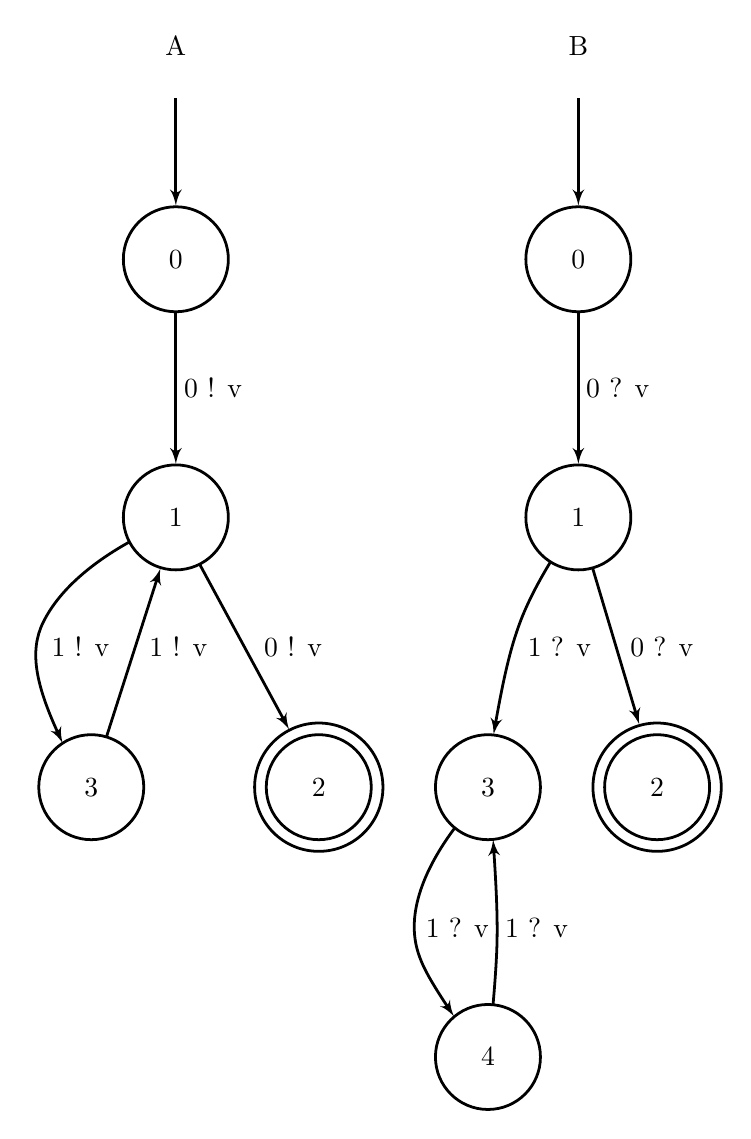
\begin{tikzpicture}[>=latex',line join=bevel,scale=1.05]
  \pgfsetlinewidth{1bp}
%%
\pgfsetcolor{black}
  % Edge: B3 -> B4
  \draw [->] (144.22bp,96.57bp) .. controls (135.94bp,85.51bp) and (126.9bp,69.041bp)  .. (131.56bp,54.0bp) .. controls (132.92bp,49.613bp) and (135.04bp,45.286bp)  .. (143.89bp,31.954bp);
  \definecolor{strokecol}{rgb}{0.0,0.0,0.0};
  \pgfsetstrokecolor{strokecol}
  \draw (145.06bp,62.25bp) node {1 ? v};
  % Edge: B4 -> B3
  \draw [->] (157.32bp,36.071bp) .. controls (157.82bp,41.766bp) and (158.31bp,48.151bp)  .. (158.56bp,54.0bp) .. controls (158.94bp,62.881bp) and (158.66bp,72.558bp)  .. (157.33bp,92.502bp);
  \draw (172.23bp,62.25bp) node {1 ? v};
  % Edge: Bdummy -> B0
  \draw [->] (186.56bp,346.67bp) .. controls (186.56bp,339.06bp) and (186.56bp,329.85bp)  .. (186.56bp,309.95bp);
  % Edge: A3 -> A1
  \draw [->] (24.844bp,127.99bp) .. controls (29.004bp,140.98bp) and (34.892bp,159.35bp)  .. (43.239bp,185.4bp);
  \draw (49.406bp,158.75bp) node {1 ! v};
  % Edge: B0 -> B1
  \draw [->] (186.56bp,273.41bp) .. controls (186.56bp,261.76bp) and (186.56bp,246.05bp)  .. (186.56bp,221.35bp);
  \draw (200.06bp,247.25bp) node {0 ? v};
  % Edge: A1 -> A2
  \draw [->] (56.87bp,186.65bp) .. controls (63.703bp,174.03bp) and (73.577bp,155.79bp)  .. (87.333bp,130.39bp);
  \draw (88.742bp,158.75bp) node {0 ! v};
  % Edge: A1 -> A3
  \draw [->] (32.341bp,194.41bp) .. controls (21.881bp,188.55bp) and (9.1337bp,179.34bp)  .. (3.0583bp,167.0bp) .. controls (-1.7681bp,157.2bp) and (0.47788bp,145.72bp)  .. (9.7171bp,125.67bp);
  \draw (15.808bp,158.75bp) node {1 ! v};
  % Edge: A0 -> A1
  \draw [->] (48.558bp,273.41bp) .. controls (48.558bp,261.76bp) and (48.558bp,246.05bp)  .. (48.558bp,221.35bp);
  \draw (61.308bp,247.25bp) node {0 ! v};
  % Edge: B1 -> B3
  \draw [->] (176.88bp,187.53bp) .. controls (173.18bp,181.42bp) and (169.2bp,174.08bp)  .. (166.56bp,167.0bp) .. controls (163.37bp,158.46bp) and (161.05bp,148.82bp)  .. (157.5bp,128.65bp);
  \draw (180.06bp,158.75bp) node {1 ? v};
  % Edge: B1 -> B2
  \draw [->] (191.51bp,185.4bp) .. controls (195.04bp,173.56bp) and (199.9bp,157.28bp)  .. (207.41bp,132.12bp);
  \draw (215.17bp,158.75bp) node {0 ? v};
  % Edge: Adummy -> A0
  \draw [->] (48.558bp,346.67bp) .. controls (48.558bp,339.06bp) and (48.558bp,329.85bp)  .. (48.558bp,309.95bp);
  % Node: A2
\begin{scope}
  \definecolor{strokecol}{rgb}{0.0,0.0,0.0};
  \pgfsetstrokecolor{strokecol}
  \draw (97.56bp,110.5bp) ellipse (18.0bp and 18.0bp);
  \draw (97.56bp,110.5bp) ellipse (22.0bp and 22.0bp);
  \draw (97.558bp,110.5bp) node {2};
\end{scope}
  % Node: B3
\begin{scope}
  \definecolor{strokecol}{rgb}{0.0,0.0,0.0};
  \pgfsetstrokecolor{strokecol}
  \draw (155.56bp,110.5bp) ellipse (18.0bp and 18.0bp);
  \draw (155.56bp,110.5bp) node {3};
\end{scope}
  % Node: B4
\begin{scope}
  \definecolor{strokecol}{rgb}{0.0,0.0,0.0};
  \pgfsetstrokecolor{strokecol}
  \draw (155.56bp,18.0bp) ellipse (18.0bp and 18.0bp);
  \draw (155.56bp,18.0bp) node {4};
\end{scope}
  % Node: Bdummy
\begin{scope}
  \definecolor{strokecol}{rgb}{0.0,0.0,0.0};
  \pgfsetstrokecolor{strokecol}
  % \draw (186.56bp,364.5bp) ellipse (27.0bp and 18.0bp);
  \draw (186.56bp,364.5bp) node {B};
\end{scope}
  % Node: B0
\begin{scope}
  \definecolor{strokecol}{rgb}{0.0,0.0,0.0};
  \pgfsetstrokecolor{strokecol}
  \draw (186.56bp,291.5bp) ellipse (18.0bp and 18.0bp);
  \draw (186.56bp,291.5bp) node {0};
\end{scope}
  % Node: A3
\begin{scope}
  \definecolor{strokecol}{rgb}{0.0,0.0,0.0};
  \pgfsetstrokecolor{strokecol}
  \draw (19.56bp,110.5bp) ellipse (18.0bp and 18.0bp);
  \draw (19.558bp,110.5bp) node {3};
\end{scope}
  % Node: A1
\begin{scope}
  \definecolor{strokecol}{rgb}{0.0,0.0,0.0};
  \pgfsetstrokecolor{strokecol}
  \draw (48.56bp,203.0bp) ellipse (18.0bp and 18.0bp);
  \draw (48.558bp,203.0bp) node {1};
\end{scope}
  % Node: B1
\begin{scope}
  \definecolor{strokecol}{rgb}{0.0,0.0,0.0};
  \pgfsetstrokecolor{strokecol}
  \draw (186.56bp,203.0bp) ellipse (18.0bp and 18.0bp);
  \draw (186.56bp,203.0bp) node {1};
\end{scope}
  % Node: B2
\begin{scope}
  \definecolor{strokecol}{rgb}{0.0,0.0,0.0};
  \pgfsetstrokecolor{strokecol}
  \draw (213.56bp,110.5bp) ellipse (18.0bp and 18.0bp);
  \draw (213.56bp,110.5bp) ellipse (22.0bp and 22.0bp);
  \draw (213.56bp,110.5bp) node {2};
\end{scope}
  % Node: A0
\begin{scope}
  \definecolor{strokecol}{rgb}{0.0,0.0,0.0};
  \pgfsetstrokecolor{strokecol}
  \draw (48.56bp,291.5bp) ellipse (18.0bp and 18.0bp);
  \draw (48.558bp,291.5bp) node {0};
\end{scope}
  % Node: Adummy
\begin{scope}
  \definecolor{strokecol}{rgb}{0.0,0.0,0.0};
  \pgfsetstrokecolor{strokecol}
  % \draw (48.56bp,364.5bp) ellipse (27.0bp and 18.0bp);
  \draw (48.558bp,364.5bp) node {A};
\end{scope}
%
\end{tikzpicture}
    \caption{SCM automata representation of the Example~\ref{exm:loop}.}
    \label{fig:loop}
\end{figure}


\begin{figure}[!ht]
    \centering

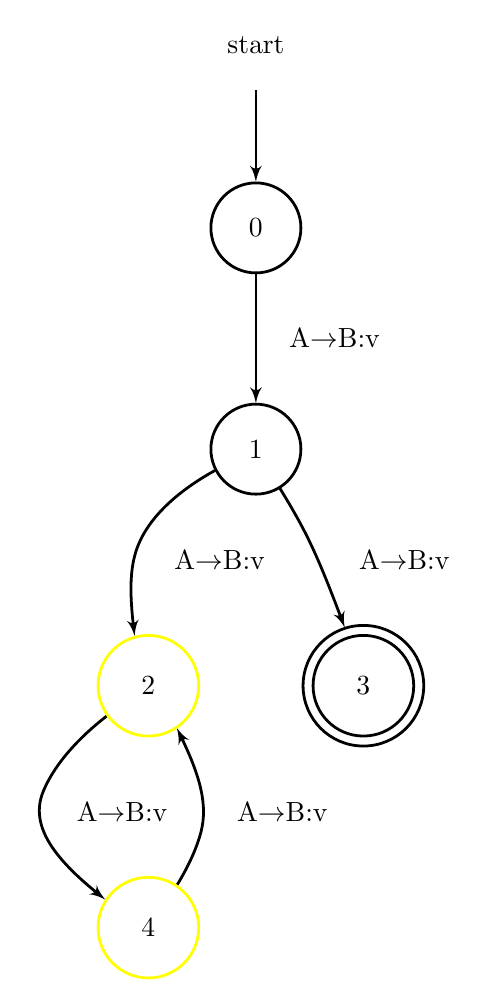
\begin{tikzpicture}[>=latex',line join=bevel,scale=0.9]
  \pgfsetlinewidth{1bp}
%%
\pgfsetcolor{black}
  % Edge: A3B3 -> A1B4
  \draw [->] (27.548bp,105.03bp) .. controls (18.113bp,97.729bp) and (7.1099bp,87.181bp)  .. (1.8895bp,74.762bp) .. controls (-3.8439bp,61.122bp) and (6.0577bp,48.005bp)  .. (26.676bp,31.31bp);
  \definecolor{strokecol}{rgb}{0.0,0.0,0.0};
  \pgfsetstrokecolor{strokecol}
  \draw (33.39bp,66.512bp) node {A$\to$B:v};
  % Edge: A0B0 -> A1B1
  \draw [->] (86.89bp,281.93bp) .. controls (86.89bp,270.28bp) and (86.89bp,254.57bp)  .. (86.89bp,229.87bp);
  \draw (118.39bp,255.77bp) node {A$\to$B:v};
  % Edge: start_node -> A0B0
  \draw [->] (86.89bp,355.2bp) .. controls (86.89bp,347.59bp) and (86.89bp,338.37bp)  .. (86.89bp,318.47bp);
  % Edge: A1B1 -> A3B3
  \draw [->] (70.499bp,202.98bp) .. controls (59.926bp,197.13bp) and (47.04bp,187.93bp)  .. (40.89bp,175.52bp) .. controls (36.728bp,167.13bp) and (36.008bp,157.18bp)  .. (38.379bp,136.75bp);
  \draw (72.39bp,167.27bp) node {A$\to$B:v};
  % Edge: A1B1 -> A2B2
  \draw [->] (96.475bp,195.86bp) .. controls (100.28bp,189.71bp) and (104.54bp,182.41bp)  .. (107.89bp,175.52bp) .. controls (111.69bp,167.71bp) and (115.29bp,159.06bp)  .. (122.42bp,140.17bp);
  \draw (146.28bp,167.27bp) node {A$\to$B:v};
  % Edge: A1B4 -> A3B3
  \draw [->] (55.235bp,36.979bp) .. controls (59.096bp,43.289bp) and (62.929bp,50.814bp)  .. (64.89bp,58.262bp) .. controls (67.676bp,68.85bp) and (64.837bp,80.229bp)  .. (55.255bp,99.999bp);
  \draw (97.489bp,66.512bp) node {A$\to$B:v};
  % Node: A3B3
\begin{scope}
  \definecolor{strokecol}{rgb}{1.0,1.0,0.0};
  \pgfsetstrokecolor{strokecol}
  \draw (43.89bp,116.89bp) ellipse (20.13bp and 20.13bp);
  \definecolor{strokecol}{rgb}{0.0,0.0,0.0};
  \pgfsetstrokecolor{strokecol}
  \draw (43.89bp,116.89bp) node {2};
\end{scope}
  % Node: A1B4
\begin{scope}
  \definecolor{strokecol}{rgb}{1.0,1.0,0.0};
  \pgfsetstrokecolor{strokecol}
  \draw (43.89bp,20.13bp) ellipse (20.13bp and 20.13bp);
  \definecolor{strokecol}{rgb}{0.0,0.0,0.0};
  \pgfsetstrokecolor{strokecol}
  \draw (43.89bp,20.131bp) node {4};
\end{scope}
  % Node: A2B2
\begin{scope}
  \definecolor{strokecol}{rgb}{0.0,0.0,0.0};
  \pgfsetstrokecolor{strokecol}
  \draw (129.89bp,116.89bp) ellipse (20.13bp and 20.13bp);
  \draw (129.89bp,116.89bp) ellipse (24.13bp and 24.13bp);
  \draw (129.89bp,116.89bp) node {3};
\end{scope}
  % Node: A0B0
\begin{scope}
  \definecolor{strokecol}{rgb}{0.0,0.0,0.0};
  \pgfsetstrokecolor{strokecol}
  \draw (86.89bp,300.02bp) ellipse (18.0bp and 18.0bp);
  \draw (86.89bp,300.02bp) node {0};
\end{scope}
  % Node: A1B1
\begin{scope}
  \definecolor{strokecol}{rgb}{0.0,0.0,0.0};
  \pgfsetstrokecolor{strokecol}
  \draw (86.89bp,211.52bp) ellipse (18.0bp and 18.0bp);
  \draw (86.89bp,211.52bp) node {1};
\end{scope}
  % Node: start_node
\begin{scope}
  \definecolor{strokecol}{rgb}{0.0,0.0,0.0};
  \pgfsetstrokecolor{strokecol}
  \draw (86.89bp,373.02bp) node {start};
\end{scope}
%
\end{tikzpicture}

    \caption{Synchronous Product of the Loop Example~\ref{exm:loop}}
    \label{fig:loop-sync}
\end{figure}


\end{example}


\chapter{Related work}\label{sec:rel}
This chapter reviews related work on the \emph{realisability problem} 
for \emph{global types}, both within the same theoretical framework 
and in closely related models.  
The idea of using communicating automata for global types is already 
well established and adopted in various frameworks. Our approach 
adopts an automata-based definition of global types, which captures a 
set of MSCs parameterised by the desired communication semantics.  
This follows the line of research initiated in~\cite{di2023partial} 
and extended in~\cite{di2025realisability}, which aims to establish a 
general framework for communication semantics.  

We have already presented in this thesis the asynchronous 
(\verb|asy|), peer-to-peer (\verb|p2p|), and synchronous 
(\verb|sync|) communication semantics.  
Furthermore, \cite{di2023partial} discusses additional semantics, 
among which the causal order (\verb|co|) and mailbox (\verb|mb|) 
semantics are particularly relevant.
In the causal order model, messages are delivered according 
to their causal dependencies: if $m_1$ causally precedes $m_2$, then 
$m_1$ must be received first~\cite{lamport2019time}.  
Causality, formalised by Lamport’s ``happened-before'' relation, ensures 
consistent delivery order and can be implemented using logical clocks.  
In the mailbox model, all messages sent to the same process, 
regardless of sender, must be received in the order they were sent, 
effectively enforcing FIFO delivery per receiver.  

\cite{di2023partial} also introduces a hierarchy of communication 
semantics, illustrated in a slightly modified form in 
Figure~\ref{fig:coms}.  
The main objective of this work was to establish a hierarchy that 
preserves \emph{monotonic} properties: if a property holds for a given 
communication semantic, it should also hold for all semantics 
contained within it.  
However, it was shown that this monotonicity applies only to specific 
properties, such as \emph{weakly-$k$-synchronisability}~\cite{di2023partial}.  
In contrast, it does not generally extend to the realisability 
problem, which is why we focused on the problem for specific semantics, 
namely peer-to-peer and synchronous communication.

\bigskip

\begin{figure}[!ht]
\centering
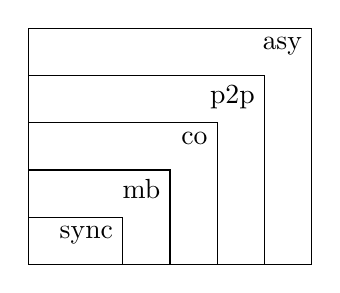
\begin{tikzpicture}[scale=0.6]
  % list of labels in order (from smallest to largest)
%   \def\labels{{rsc,nn,onen,mb,co,p2p,asy}}
  % loop to draw nested squares
  \foreach [count=\i] \lab in {sync,mb,co,p2p,asy} {
    \draw (0,0) rectangle (\i+1,\i);
    \node[anchor=north east] at (\i+1,\i) {\lab};
  }
\end{tikzpicture}
\caption{Hierarchy of communication model semantics.}
\label{fig:coms}
\end{figure}

We then examine recent advances by
Stutz~et~al.~\cite{stutz2024implementability}, who provide a
comprehensive automata-theoretic treatment of the realisability problem,
and trace this line of inquiry back to early results by
Alur~et~al.~\cite{alur2000inference} and
Lohrey~et~al.~\cite{lohrey2003realizability}.  
Finally, we consider formalisms related to Multiparty Session Types
(MPST), such as Choreography Automata~\cite{barbanera2020choreography},
highlighting conceptual connections and key differences with the
approach developed in this thesis.

\section{Realisability of MSCs and HMSCs}
In this section, we compare our framework with one of the earliest and
most influential works on realisability, the one of 
Alur~et~al.~\cite{alur2005realizability}, which also inspired part of our
approach. Their notion of \emph{Weak Realisability} captures the idea that
a specification of Message Sequence Charts (MSCs) should already include
all behaviours that are consistent with the local views of processes. 
Intuitively, a set of MSCs is weakly realisable when, for every process,
the events it observes in any MSC of the specification are compatible
with those in some MSC already in the set. This closure condition ensures
that the global behaviour can be reconstructed from the projections of
individual processes, so that every implied MSC is already part of the
language. 
% Alur~et~al. also provided an equivalent characterisation of
% weak realisability in terms of closure over prefixes of MSCs. 
Our own definition
of weak realisability coincides with theirs, as it expresses the same
fidelity concept over the local behaviour and abstracts from any
deadlock-related concern. In both cases, weak realisability focuses on
the alignment between local and global behaviours rather than on safety
properties such as deadlock-freedom. For safe realisability, we recall an
informal definition of Alur~et~al.~\cite{alur2005realizability} and discuss
the differences.

Intuitively, let $L$ be a set of MSCs. Then $L$ is said to be 
\emph{safely realisable} if there exists a family of communication automata 
$\langle A_i \mid 1 \leq i \leq n \rangle$ such that $L = L(\prod_i A_i)$ 
and the product automaton $\prod_i A_i$ is \emph{deadlock-free}. 
In this setting, a \emph{deadlock state} is a configuration of the global 
system from which no accepting state can be reached. 
This corresponds to a situation where all processes are 
waiting to receive messages that are no longer available in their 
communication buffers, preventing further progress. 
Hence, a system is deadlock-free if no such state is reachable from its 
initial configuration. This notion captures the safety aspect of 
realisability by ensuring that the system never reaches a globally 
stalled state during execution. This definition of safe realisability 
corresponds to ours in $\ppmodel$ or $\synchmodel$.

The work of Alur~et~al.~went on further, defining specific complexity classes 
for different kinds of assumptions. For finite sets of MSCs,
weakly realisability is shown to be \verb|coNP|-complete and safe 
realisability is shown to be decidable in \verb|P|-time. The problem
was subsequently studied for HMSCs. For \emph{bounded} HMSCs, safe realisability 
remains decidable, and it is \verb|EXPSPACE|-complete, but weak realisability 
becomes undecidable. For \emph{unbounded} HMSCs, 
safe realisability remains decidable, and it is \verb|EXPSPACE|-complete, but weak realisability 
becomes undecidable~\cite{alur2005realizability}. 
Later, Lohrey~et al.~\cite{lohrey2003realizability} proved in the general case, 
with a technique that involves five processes, that safe realisability 
is undecidable, though it is decidable (and \verb|EXPSPACE|-complete) 
for a specific kind of HMSCs, called globally-cooperative HMSCs, introducted 
in \cite{morin2002recognizable}.
Furthermore, in the context of weak realisability,
Genest et~al.~\cite{genest2006infinite} introduced the notion of
\emph{locally-cooperative} HMSCs, for which implementability can be
checked in linear time.
Since every globally-cooperative HMSC is also locally-cooperative,
verifying implementability for this broader class remains at least
\verb|EXPSPACE|-hard, if it is decidable at all.
Lohrey~et al.~\cite{lohrey2003realizability} also considered another subclass of HMSC,
called $\mathcal{I}$-closed HMSC, whose checking of safe realisability is \verb|PSPACE|-complete.
Most positive results assume other struttural restrictions, like bounded channels, 
but \cite{bollig2025high} introduces a new class of loop-connected HMSCs
that allows unbounded channels while maintaining realisability.
Table~\ref{tab:realisability-summary} summarises the results presented in this section.

\section{Session Types}
Session Types provide a type-theoretic framework for specifying and verifying 
communication protocols among multiple participants.  
They ensure that interactions follow a predefined structure, 
preventing common concurrency errors such as deadlocks, orphan messages, 
and unspecified receptions. 
Session types were first formalised as 
\emph{Binary Session Types}~\cite{honda1993types}, 
which capture structured communication between two peers.  
The framework later evolved into 
\emph{Multiparty Session Types (MPST)}~\cite{honda2008multiparty}, 
extending the theory to interactions among multiple participants.  
Over the years, session types have been integrated into several programming 
languages~\cite{DBLP:journals/ftpl/AnconaBB0CDGGGH16}, including 
Rust~\cite{jespersen2015session,chen2020ferrite}, 
Haskell~\cite{lindley2016embedding}, 
Erlang~\cite{mostrous2011session}, and
Ocaml~\cite{padovani2017simple}
broadening their practical relevance beyond purely theoretical models.  
They have also found applications across diverse domains such as 
operating systems~\cite{fahndrich2006language}, 
web services~\cite{yoshida2013scribble}, 
distributed algorithms~\cite{kouzapas2024session}, 
and smart contracts~\cite{das2021resource}.  

To sum up, the typical use of MPST involves defining a protocol through 
a \textbf{global type}, from which the \textbf{local types} of each 
participant are derived via a \emph{projection operation}.  
The system implementation, composed of communicating processes, is 
then verified against these local specifications using a 
\emph{typing system}, ensuring safe behaviour and additional properties 
such as deadlock-freedom.
% A key component of classical MPST is the \emph{merge operator}, 
% which resolves non-determinism when projecting away interactions 
% irrelevant to a participant.  
% Since merging is only partially defined, it determines whether local 
% states can be safely combined; when projection succeeds, it guarantees 
% both deadlock freedom and protocol fidelity.  
Figure~\ref{fig:mpstschema} summarises the main elements of this framework.


\begin{figure}[!ht]
\centering
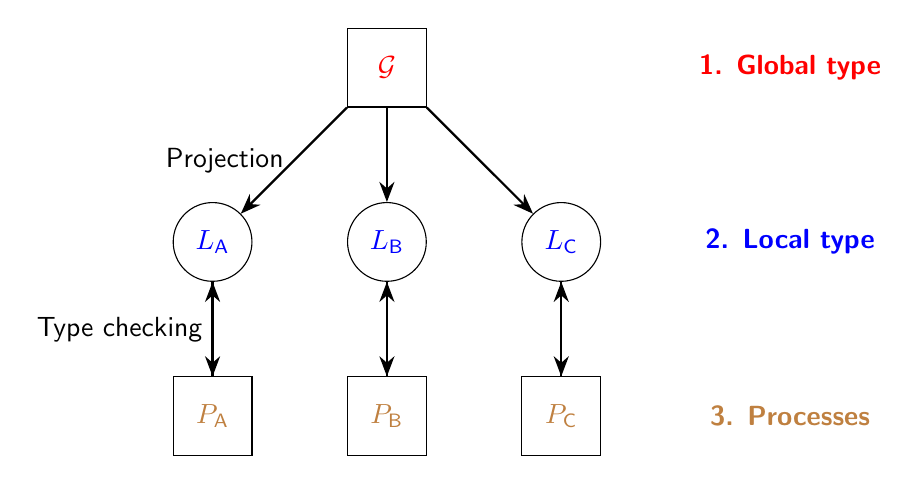
\begin{tikzpicture}[
      node distance=1.2cm,
      every node/.style={font=\sffamily},
      rect/.style={rectangle, draw=black, minimum width=1cm, minimum height=1cm},
      circ/.style={circle, draw=black, minimum size=1cm},
      arrow/.style={-{Stealth[scale=1.1]}, thick}
  ]

  % Nodes
  \node[rect] (G) {\textcolor{red}{$\mathcal{G}$}};
  \node[circ, below=of G] (TB) {\textcolor{blue}{$L_\text{B}$}};
  \node[circ, left=of TB] (TA) {\textcolor{blue}{$L_\text{A}$}};
  \node[circ, right=of TB] (TC) {\textcolor{blue}{$L_\text{C}$}};

  \node[rect, below=of TA] (PA) {\textcolor{brown}{$P_\text{A}$}};
  \node[rect, below=of TB] (PB) {\textcolor{brown}{$P_\text{B}$}};
  \node[rect, below=of TC] (PC) {\textcolor{brown}{$P_\text{C}$}};

  \node[rect,draw=none,right=of TC] (LC) {\textbf{\textcolor{blue}{2. Local type}}};
  \node[rect,draw=none,above=of LC] (LG) {\textbf{\textcolor{red}{1. Global type}}};
  \node[rect,draw=none,below=of LC] (LG) {\textbf{\textcolor{brown}{3. Processes}}};

  % Arrows
  \draw[arrow] (G) -- (TA) node[midway, left] {Projection};
  \draw[arrow] (G) -- (TB);
  \draw[arrow] (G) -- (TC);

  \draw[arrow] (PA) -- (TA) node[midway, left] {Type checking};
  \draw[arrow] (PB) -- (TB);
  \draw[arrow] (PC) -- (TC);
  \draw[arrow] (TC) -- (PC);
  \draw[arrow] (TB) -- (PB);
  \draw[arrow] (TA) -- (PA);

\end{tikzpicture}
\caption{Intuitive schema of MPST framework}
\label{fig:mpstschema}
\end{figure}

\subsection{Projectability}
\emph{Projectability} asks whether a global type can be faithfully 
projected into local specifications for each participant so that the 
resulting local types interact without mismatches or unintended 
behaviours.  
It corresponds to the \emph{realisability} problem studied in 
automata-theoretic settings, both concern whether a global specification 
admits a correct distributed implementation.

However, classical projection algorithms often reject natural yet safe 
protocols because of strong syntactic constraints designed to ensure 
safety.  
This gap between expressiveness and implementability has motivated the 
search for more permissive definitions.  
Notably, the algorithm of Castagna et al.~\cite{castagna2012global} 
was the first to aim for \emph{full completeness}, balancing safety 
and expressiveness.

\subsubsection{Realisability and Restrictions in MPST}
Recent work connects MPST with automata-theoretic models such as High-level 
Message Sequence Charts (HMSCs). Stutz and Zufferey demonstrated that 
realisability is \textbf{decidable} for global types encoded as 
\emph{globally cooperative} HMSCs~\cite{DBLP:journals/corr/abs-2209-10328,DBLP:conf/ecoop/Stutz23}.  
Li et al.~\cite{li2023complete} later introduced a complete projection operator 
ensuring correctness for all implementable global types.  

In his thesis, Stutz~\cite{stutz2024implementability} provides a comprehensive 
classification of the \textbf{syntactic restrictions} that govern both 
\emph{expressiveness} and \emph{decidability} in MPST.  
He generalises the traditional notion of sender-driven choice to allow a sender 
to branch towards different receivers, capturing common distributed patterns 
such as load balancing, while keeping the implementability 
problem \textbf{decidable} in \verb|PSPACE|.  
This establishes the first tight complexity bound for the class of 
sender-driven global types and confirms that they can be faithfully 
represented as HMSCs.  
Note that Stutz~et~al.\ interpret \emph{deadlocks} in the sense of our
\emph{progress} property, and additionally define \emph{soft deadlocks}
for its model.
The latter gives rise to the \emph{soft implementability} problem.

A key syntactic dimension in MPST is how \emph{choice} is handled 
when a branch of the protocol is encountered, as this 
determines whether projection remains decidable.  
The three main variants are:
\begin{itemize}
    \item \emph{Directed choice}: every branch shares the same 
    sender–receiver pair, yielding a single decision point.  
    This ensures safety and straightforward projection but severely limits 
    expressiveness, as many distributed coordination patterns are 
    excluded~\cite{honda2008multiparty}.  

    \item \emph{Sender-driven choice}: each branch has a single sender, 
    but receivers may differ across branches.  
    This generalisation captures richer interaction schemes while retaining 
    decidability; as mentioned, safe realisability for this fragment lies in 
    \verb|PSPACE|~\cite{stutz2024implementability}.  

    \item \emph{Mixed choice}: multiple senders may initiate branches 
    concurrently, removing a unique decision-maker.  
    While this maximises expressiveness, it introduces intrinsic 
    nondeterminism in control flow, making implementability and its 
    weaker variants (e.g., soft or weak realisability) \textbf{undecidable} 
    in general~\cite{stutz2024implementability}.  
\end{itemize}

These results precisely delineate the boundary between expressiveness and 
decidability in MPST.  
Stutz’s framework provides the first complete algorithmic account of 
implementability for sender-driven global types and proves that no 
complete algorithm can exist once mixed choice is permitted.


\section{Choreographies}
Choreographies \cite{ws-cdl-2005} and Choreographic 
Programming~\cite{montesi2014choreographic, giallorenzo2024choral, cruz2022functional} 
are other formalisms to describe  
distributed communication protocols. Choreographies emphasize the 
global specification of interactions as a high-level description of the 
intended message exchanges. Similarly to MPST, their goal is to ensure that
a distributed implementation can be derived in which each participant 
follows a local behaviour consistent with the global description, called
respectively \emph{local} and \emph{global}-view. This setting naturally 
connects to the realisability problem, since the key question is whether 
a choreography can be faithfully implemented by a system of local 
processes. 
In choreographies, the local-view is called 
\textbf{End-Point Projection} (EPP),
and it is derived via a projection operation from the global-view.
In particular, \emph{Choreography Automata}~\cite{barbanera2020choreography}  
share many conceptual similarities with our notion of Global Types.  
Both formalisms model global interaction structures through automata  
over communication actions, capturing the causal dependencies among  
participants. The main difference lies in the underlying semantics and  
the intended use: Choreography Automata focus on synthesis and  
verification within choreographic frameworks, while our Global Types  
are tailored to the study of realisability under different
communication semantics.  

One important challenge studied in choreographic design is the 
\textbf{knowledge of choice} problem~\cite{lanese2008bridging, castagna2012global}. 
This problem can be seen as a 
specific instance of the general projection problem: it arises when 
translating a global description into consistent local behaviours. 
In particular, it captures the difficulty of maintaining coherence 
when decisions made by one participant must be known by others.  

Informally, a choreography has knowledge of choice if, whenever a 
branching (conditional) decision is made by one participant, all 
other affected participants are made aware of that decision. Without 
proper communication of the choice, a participant may behave 
inconsistently because it lacks information to distinguish which 
branch was taken. For example, if process \(A\) chooses between two 
branches that lead to different sub-protocols with process \(B\), 
then \(B\) must receive a signal (a ``selection'') that lets it 
synchronize on the correct continuation.  

If the choreography lacks such a mechanism, it becomes 
\emph{unprojectable}: EPP is not allowed to generate local behaviours 
that coordinate the branching uncorrectly. This issue 
is addressed, typically, by adding explicit selection messages to 
propagate the choice, and how this can be automated via 
\emph{amendment} or \emph{repair} algorithms 
\cite{DBLP:journals/corr/LaneseMZ13, basu2016automated}, 
which insert minimal extra 
communications to guarantee knowledge of choice.  

Conceptually, this problem is closely related to the \emph{sender-driven 
choice} policy highlighted before in the MPST framework, where 
multiple senders make independent choices that must be reconciled to 
ensure a coherent global behaviour. In both cases, the challenge lies 
in ensuring that all participants have sufficient knowledge to follow 
the same branch, preserving consistency across local projections. 


\section{Other works}
In his thesis~\cite{stutz2024implementability}, 
Stutz further investigate which syntactic and semantic
restrictions in global types are \emph{non-restrictive}, that is, those that
do not compromise expressiveness while preserving decidability.  
Stutz et al.~introduce
\emph{Protocol State Machines} (PSMs)~\cite{stutz2025automata}, 
a unifying automata-theoretic
formalism that strictly generalises both Global Types and HMSCs.  
This model captures interaction protocols as communicating state
machines over message-passing labels, bridging automata theory and MPST.
His results show that every sink-final $\Sigma 1$-PSM can be represented
as a non-deterministic Global Type that preserves sender-driven or
mixed-choice behaviour~\cite[Thm.~8.14]{stutz2024implementability}.  
Later, Stutz et~al.~\cite{stutz2025automata} extended this line of work,
formalising PSMs and analysing the computational complexity of type
checking and realisability. They demonstrate that, for choice-free or
single-choice fragments, both problems remain decidable (often in
\verb|PTIME|), whereas the introduction of \emph{mixed choice} renders
realisability \emph{undecidable}.  
Together, these results reinforce the view that structural constraints
such as single recursion points or explicit termination are
\emph{expressively harmless}, while the distinction between
\emph{sender-driven} and \emph{mixed} choice constitutes the true
boundary between decidability and undecidability in distributed protocol
implementations.

Another relevant contribution is by Guanciale et al.~ 
\cite{DBLP:journals/jlap/GuancialeT19}, who study the 
\emph{realisability of pomsets} via communicating automata. 
Pomsets, or partially ordered multisets, generalise MSCs by 
capturing causal dependencies among events rather than total 
orders. Their work defines realisability conditions ensuring 
both communication correctness and termination soundness, 
supporting participants with internal concurrency.
Table~\ref{tab:realisability-summary} summarises the 
main results analised in the last sections. To our knowledge, 
empty cells are to be considered open problems, like
the safe realisability problem for sender-driven HMSCs
and PSMs.

\bigskip

\begin{table}[!ht]
\centering
\renewcommand{\arraystretch}{1.3}
\begin{tabular}{|p{4.3cm}|p{4.3cm}|p{4.3cm}|}
\hline
\textbf{Formal Model} & \textbf{Weak Realisability} & \textbf{Safe Realisability} \\ 
\hline
\textbf{Finite sets of MSCs} 
& coNP-complete~\cite{alur2005realizability} 
& P-time~\cite{alur2005realizability} \\ 
\hline
\textbf{Unbounded HMSCs} 
& Undecidable~\cite{lohrey2003realizability} 
& Undecidable~\cite{lohrey2003realizability} \\ 
\hline
\textbf{Bounded HMSCs (FIFO)} 
& Undecidable~\cite{alur2005realizability} 
& EXPSPACE-complete~\cite{lohrey2003realizability} \\ 
\hline
\textbf{Bounded HMSCs (non-FIFO)} 
& Decidable~\cite{morin2002recognizable} 
& EXPSPACE-complete~\cite{lohrey2003realizability} \\ 
\hline
\textbf{Globally-Cooperative HMSCs} 
& -- 
& EXPSPACE-complete~\cite{morin2002recognizable} \\ 
\hline
\textbf{Locally-Cooperative HMSCs} 
& Linear time~\cite{genest2006infinite}
& At most EXPSPACE-complete~\cite{morin2002recognizable}  \\ 
\hline
\textbf{$\mathcal{I}$-Closed HMSCs} 
& -- 
& PSPACE-complete~\cite{lohrey2003realizability} \\ 
\hline
\textbf{Loop-connected HMSCs (unbounded channels)} 
& Decidable~\cite{bollig2025high}
& -- \\ 
\hline
\textbf{MPST (directed choice)} 
& --
& Decidable, but incomplete~\cite{honda2008multiparty} \\ 
\hline
\textbf{MPST (sender-driven choice)} 
& --
& PSPACE-complete~\cite{stutz2024implementability} \\ 
\hline
\textbf{MPST (mixed choice)} 
& Undecidable~\cite{stutz2024implementability} 
& Undecidable~\cite{stutz2024implementability} \\ 
\hline
\textbf{General PSMs} 
& --
& Undecidable~\cite{stutz2025automata} \\ 
\hline
\textbf{Choreographic Programming} 
& --
& Decidable~\cite{barbanera2020choreography} \\ 
\hline
\end{tabular}
\caption{Summary of computational complexity for weak and safe realisability across formal models.}
\label{tab:realisability-summary}
\end{table}

\section{Related Tools}\label{sec:reltool}
Several verification tools have been developed to analyse communicating 
automata and distributed systems under asynchronous or bounded communication 
semantics. 

\textsc{McScM}~\cite{heussner2012mcscm} is the tool most closely related 
to \textsc{ReSCu}. It takes as input a system description and a set of 
\emph{bad configurations} (expressed using Queue Decision Diagrams, QDDs, 
from~\cite{boigelot1996symbolic}) and checks their reachability. 
The tool implements multiple model-checking strategies based on abstract 
interpretation~\cite{cousot1977abstract} and supports general classes of communicating systems.  
In contrast to \textsc{ReSCu}, most approaches in \textsc{McScM} are 
\emph{semi-algorithms}, requiring user-defined timeouts to terminate.  
However, its strength lies in providing a diverse set of verification 
engines, which increases the likelihood of obtaining conclusive verification 
results.  
Notably, \textsc{ReSCu} reuses the same input description language as 
\textsc{McScM}, ensuring compatibility and easing system specification.

\textsc{KMC}~\cite{lange2019verifying} (for \emph{k-Multiparty 
Compatibility}) was introduced by Lange and Yoshida to verify whether a 
system could have been derived from a \emph{Multiparty Session Type} (MPST).  
If a system satisfies $k$-MC, several safety properties, such as freedom from 
deadlock and orphan messages, are guaranteed automatically.  
Unlike \textsc{ReSCu} and \textsc{McScM}, \textsc{KMC} does not require the 
explicit specification of safety conditions but relies on the theoretical 
guarantees of MPST projection.

The \textsc{STaB-C} tool~\cite{akroun2018automated,akroun2016automated} 
implements semi-algorithms for checking \emph{k-stability}, a property that 
guarantees behavioural equivalence across different communication bounds.  
A system is $k$-stable if, for any larger bound $k' > k$, its behaviour 
remains equivalent (under various notions of trace or observational 
equivalence).  
While \textsc{STaB-C} focuses on detecting stability rather than verifying 
safety or liveness, it provides important insight into boundedness and 
behavioural robustness of FIFO systems.  
Unlike \textsc{ReSCu}, which verifies multiple semantic properties such as 
deadlock-freedom and progress, \textsc{STaB-C} focuses exclusively on 
membership in the class of $k$-stable systems.


\chapter{Conclusion}\label{sec:end}
This work addressed the \emph{realisability problem} for Global 
Types, a central concern in the verification of distributed systems. 
After a brief overview of the problem, we positioned our contribution 
within an ongoing research effort, bridging well-established 
theoretical foundations with practical tool development.  

On the theoretical side, we introduced the necessary background 
notions (i.e.\ CFSMs, Global Types, MSCs, and communication models) and 
formalised weak realisability. The main contribution was to connect 
the realisability problem to classical undecidability results, in 
particular through a reduction to the Relaxed Post Correspondence 
Problem (RPCP). This result, presented in 
Chapter~\ref{sec:proof}, establishes a limitation 
of realisability under synchronous semantics and lays the groundwork 
for exploring decidable subclasses and practical approximations.

On the practical side, detailed in Chapter~\ref{sec:rescu}, we improved 
and extended the \textsc{ReSCu} tool, used for checking realisability 
and other semantic properties of Symbolic Communicating Machines 
(SCMs). The input grammar was refined for greater usability, and new 
verification routines were implemented, including checks for progress 
and deadlock-freedom. The tool now also generates visual 
representations of synchronous systems, along with illustrative 
examples. These extensions strengthen \textsc{ReSCu} both as a research 
prototype and as a practical aid for automated verification.

In Chapter~\ref{sec:rel}, we analysed part of the state of the art on 
realisability, comparing our definitions and results with existing 
approaches in the literature. This analysis helped clarify how our 
formalisation of weak and safe realisability fits within, and extends, 
previous frameworks, particularly those by 
Alur~et~al.~\cite{alur2005realizability}, 
Lohrey~et~al.~\cite{lohrey2003realizability}, and 
Stutz~et~al.~\cite{stutz2024implementability}. The comparison also 
highlighted key conceptual differences, especially in how communication 
semantics and closure properties are handled, further motivating our 
formal treatment.

\section{Future Work}
Future research directions include extending the theoretical results
beyond weak realisability toward a decidability result for
\emph{safe realisability}, therefore incorporating properties such as
deadlock-freedom directly into the analysis of global types. This line
of investigation will build upon the techniques developed in this work
and extend the existing results of Lohrey~et~al.~\cite{lohrey2003realizability}.  

Another important direction is the exploration of alternative
communication semantics, such as causal-order and mailbox-based models,
which were mentioned throughout this work. Investigating the
realisability problem under these semantics could shed light on how
communication constraints and buffering behaviours affect implementability
and decidability. Establishing precise connections between synchronous
semantics and these more general models may also lead to new transfer
results, showing under which conditions realisability in one model
implies realisability in another.  

On the practical side, a natural objective is to further enhance
\textsc{ReSCu} to support these theoretical extensions, ultimately
aiming for a complete and automated framework to decide realisability
for restricted classes of global types. This would enable systematic
benchmarking against existing tools and the validation of the approach
on real-world communication protocols.  

Finally, it would be valuable to investigate the role of \emph{fairness}
and other semantic variants, within the verification process. 
These extensions could help
model more realistic distributed environments and provide a deeper
understanding of how fairness assumptions influence the decidability and
correctness of realisable systems.


\newpage

\phantomsection
\addcontentsline{toc}{chapter}{References}
\bibliographystyle{plain}
\bibliography{ref}

% \newpage
% \begin{appendices}\label{apx}
  




\end{appendices}

\newpage

\chapter*{Acknowledgments}
\addcontentsline{toc}{chapter}{Acknowledgments}

First and foremost, I would like to thank the researchers who actively 
collaborated in writing this thesis. Above all, I wish to thank my 
internship supervisor at the laboratory in Nice, Prof. Cinzia Di Giusto, 
who, with great perseverance, demanded formal accuracy in every detail. 
Thanks to her meticulousness, I learned a lot about this profession and 
understood how important it is never to overlook anything.

I would also like to thank Prof. Ivan Lanese for his support during the 
writing of this thesis and for his valuable corrections. I am also grateful 
to Prof. Etienne Losez for the helpful and detailed preliminary discussions 
about the contributions presented in this work.

I wish to thank my parents, Riccardo and Paola, for always being there for me, 
for their unconditional love, and for giving me the freedom to make mistakes 
and grow.

I thank Eleonora for her courage in placing trust in me and in our shared life 
project, which we are building with effort but which I believe will become 
the most beautiful thing in my life.

I thank Samuele, who in his own way inspires me through his choices and 
shares with me the hassle of managing our home server.

I thank all those I met during this master’s degree, especially the friends 
from my bachelor’s years and the new ones adopted along the way: Simo Borto, 
Criss, Fede, Andreea, Simo R., Dan, DavideDarioCiro, Santo, Fusillo, Chapo, 
LP, Apo, Mario, Greg, Gaia, Andrea Ianno, and Luca Bassi. I’ve made many 
memories I will carry in my heart, from every exam we studied for together 
to the struggle of finding our own place, which we then called the 
\emph{bunker}.

I am grateful to those who gave me the opportunity to spend a year abroad in 
Nice through the Erasmus program. It was an incredible year that allowed me 
to leave home for the first time and live somewhere other than Bologna. It 
helped me grow and gave me the confidence to say that I can make it on my own. 
Thank you to Erik for sharing this adventure from the start and for being my 
personal trainer. Thanks to all the old and new \emph{ubinetters}. Through 
this experience, I met so many amazing friends to whom I owe a lot. Among the 
first, the group \emph{Metà Stivale} with Silvia, Arianna, Giuse, Niky, 
Sabri, Lucry, and Amira. The family-like atmosphere that was created was 
magical and unrepeatable.

During the wild summer period, I met some of the most fun-loving people I 
know, and I thank you all for the crazy nights, trips, and travels. Thanks 
to the \emph{Carras team}, Mary and Ana, whose flat became a second home. Thanks 
to Bence, Coleen, Dory, Hannah, Marialena, Mesi, Myriam, Pietro, Richi, 
Hugo, Joy, Isaac, Lea, and Pia for sharing this experience with me. I really 
hope to meet each of you again in the future.

Finally, thank you to my lifelong friends, who remain as anchors I can always 
rely on. Special thanks to those from my bachelor’s days: Luca, Fabio, Gian, 
and Volpe. Thanks to my friends from Bologna: Alf, Annac, Annam, Giulietta, 
Vanni, Leti, Marto, and Tommy. Thanks to my scout community, 
\emph{Bologna 13}, to the children of the \emph{branco Waingunga}, 
and to all the scout chief with 
whom I shared that journey. I sincerely hope to return to scouting in the 
future. I feel truly fortunate to have each of these people in my life.


\end{document}
